\chapter{Theorver}

\section{Вступ в теорію ймовірності}

\subsection{Математична модель ймовірнісного експерименту}

\begin{definition}
    \textbf{Ймовірнісним (статистичним) експериментом} ---
    називають експеримент, для якого:

    1) Множина можливих результатів наперед відома.

    2) Наперед знати, яким саме результатом закінчиться
    експеримент, ми не можемо.

    3) Експеримент можна повторювати як завгодно багато
    разів при однакових умовах.
\end{definition}

\begin{example}~\par
    1) Підкидання монети.

    2) Підкидання кубика.
\end{example}

\begin{definition}
    \textbf{Простором елементарних подій} експерименту,
    називають множину $\Omega$ всіх можливих результатів
    експерименту.
\end{definition}

\begin{example}
    1) Монета підкидається 1 раз.

    $\Omega = \{\omega_1, \omega_2\} 
    = \{\text{Р}, \text{Г}\}; |\Omega| = 2$

    2) Монета підкидається двіччі.

    $\Omega = \{\text{ГГ}, \text{ГР}, \text{РГ}, \text{РР}\}; |\Omega| = 4$

    3) Монету підкидають до першої появи герба.

    $\Omega = \{\text{Г}, \text{РГ}, \text{РРГ}, ...\}$
    
    $\omega_i = \underbrace{\text{РР...Р}}\limits_{i-1}\text{Г}, i = 1, 2, 3, ...$
    
    $|\Omega| = \infty, \Omega \text{ --- зліченна множина}$

    4) Задача про зустріч.

    Двоє людей домовились про зустріч в секретному місці
    між 12:00 і 13:00. Кожен з них вибирає час приходу на
    місце навмання.

    $\Omega = \{(t_1, t_2): 0 \leqslant t_1 \leqslant 1,
    0 \leqslant t_2 \leqslant 1\}$

    $t_1$ --- час прибуття 1-ої людини

    $t_1$ --- час прибуття 2-ої людини

    $\Omega$ має потужність континума.
\end{example}

\subsection{Дискретний простір елементарних подій}

Вважаємо, що $\Omega$ --- скінченна або зліченна множина.

 \begin{definition}
    Довільна підмножина $A \subseteq \Omega$ дискретного
    простору елементарних подій --- це \textbf{випадкова
    подія}.
 \end{definition}

 \begin{remark}
    Якщо $\Omega$ --- довільна (не обов'язково дискретна),
    то взагалі кажучи не кожна її підмножина є випадковою
    подією.
 \end{remark}

 Кажуть, що подія $A$ відбулася, якщо відбулася якась з 
 елементарних подій $\omega \in A$.

 \begin{example}~\par
    1) Підкидають 1 раз гральний кубик.\par
    $\Omega = \{1, 2, 3, 4, 5,6\}; |\Omega| = 6$\par
    $A = \{$Випала парна кількість очок$\}$\par
    $A = \{2, 4, 6\}, |A| = 3$

    2) Кидок 2-х гральних кубиків.\par
    $\Omega = \{(i,j), i=\overline{1,6};
        j=\overline{1,6}\}; |\Omega| = 6 \cdot 6 = 36$\par
    $A = \{$сума очок дорівнює 4$\}$\par
    $A = \{(1,3), (2,2), (3,1)\}, |A| = 3$

    3) Підкидання монети до першого герба.\par
    $\Omega = \{$Г, РГ, РРГ, ...$\}$\par
    $A = \{$Було проведено непарну кількість підкидань$\}$\par
    $A = \{\text{Г}, \text{РРГ}, ..., \underbrace{\text{Р}\cdots\text{Р}}\limits_{2k}\text{Г}, ...\}$
    $A$ --- зліченна.

    \subsection{Операції над подіями}

    1) Обєднання (сума) подій $A$ і $B$ --- це подія
    $A \cup B = \{\omega \in \Omega: \omega in A \vee \omega \in B\}$

    2) Перетин (добуток) подій $A$ і $B$ --- це подія
    $A \cap B = \{\omega \in \Omega: \omega in A \wedge \omega \in B\}$
    --- відбулися обидві події.

    3) $A \setminus B = \{\omega \in \Omega: \omega in A \wedge \omega \notin B\}$
    --- відбулась подія $A$, але не відбулася подія $B$.

    $$A \setminus B = A \cap \underline{B}$$

    4) $A \subset B$ --- з події $A$ випливає подія $B$.
 \end{example}

\begin{definition}~\par
    1) Подія $\Omega$ називається достовірною подією.
    
    2) Подія $\varnothing \subset \Omega$ називається неможливою
    подією.

    3) Подія $\overline{A} = \Omega \setminus A$ називається
    протилежною до події $A$.

    4) Події $A$ і $B$ називаються несумісними, якщо
    $A \cap B = \varnothing$
\end{definition}

\begin{example}
    Підкидають два гральних кубика.

    $\Omega = \{(i,j), i=\overline{1,6}, j=\overline{1,6}\}$

    $A = \{$сума очок дорівнює 4$\}$

    $A = \{(1,3), (2,2), (3,1)\}$

    $B = \{$на першому кубику 6 очок$\}$

    $B = \{(6,j), j = \overline{1,6}\}$

    $A \cap B = \varnothing \Rightarrow A$ і $B$ несумісні.
\end{example}

\begin{remark}
    До подій, як до множини, можна застосувати правила де
    моргана:

    а) $\overline{\bigcup\limits_{i=1}^n A_i}
    = \bigcap\limits_{i=1}^n \overline{A_i}$

    б) $\overline{\bigcap\limits_{i=1}^n A_i}
    = \bigcup\limits_{i=1}^n \overline{A_i}$
\end{remark}

\subsection{Ймовірність випадкової події}

Вважаємо, що $\Omega$ --- дискретна множина. Кажуть, що на 
$\Omega$ задано розподіл ймовірностей, якщо кожній елементарній
події $\omega \in \Omega$ ставиться у відповідність число
$P(\omega)$ так, що:

1) $\forall \omega \in \Omega: P(\omega) \geqslant 0$

2) $\sum\limits_{\omega \in \Omega} P(\omega) = 1$ --- умова
нормування.

Тоді для довільної випадкової події $A \subseteq \Omega:$

$$P(A) = \sum\limits_{\omega \in A} P(\omega)$$

$P(A)$ називається ймовірністю події $A$.

\subsubsection*{Властивості ймовірності:}~

1) $P(\Omega) = 1$ --- випливає з умови нормування, (2)

2) $P(\varnothing) = 0$

3) $P(A \cup B)
= \sum\limits_{\omega \in A \cup B} P(\omega)
= \sum\limits_{\omega \in A} P(\omega)
    + \sum\limits_{\omega \in B} P(\omega)
    - \sum\limits_{\omega \in A \cap B} P(\omega)
= P(A) + P(B) - P(A \cap B)$

Для несумісних подій ($A \cap B = \varnothing$)
$P(A \cup B) = P(A) + P(B)$

4) $P(\overline{A})
= \sum\limits_{\omega \in \overline{A}} P(\omega)
= \sum\limits_{\omega \in \Omega \setminus A} P(\omega)
= 1 - P(A)$

\subsection{Класична модель}

Якщо $|\Omega| = N$ і всі елементарні події вважаються
рівноімовірними, тобто

$P(\omega_1) = ... = P(\omega_N) = \dfrac{1}{N}$,

то $\forall A \subseteq \Omega$:

$P(A)
= \sum\limits_{\omega \in A} \dfrac{1}{N}
= \dfrac{1}{N} |A|
= \dfrac{|A|}{|\Omega|}$

--- відношення кількості сприятливих елементарних подій для
$A$ до загальної кількості елементарних подій.

\begin{example}~\par
    1) Підкидаємо симетричну монету

    $\Omega = \{\text{Р}, \text{Г}\}$

    Нехай $P(\text{Р}) = \dfrac{1}{2}$,
    $P(\text{Г}) = \dfrac{1}{2}$ --- припущення що до
    симетричності монети.

    Якщо $P(\text{Р}) = p$, $P(\text{Г}) = (1-p)$, де
    $p \neq \dfrac{1}{2}$, то монета несиметрична.

    2) Монету підкидають $n$ разів, фіксована кількість.

    $\Omega = \{(\varepsilon_1, \varepsilon_2, ..., \varepsilon_n), \varepsilon_i = 0,1\}$,
    де $\varepsilon_i = 0$, якщо випала решка в $i$-тому
    підкиданні, $\varepsilon_i = 1$, якщо випав герб.

    $|\Omega| = 2^n$

    Покладемо: $P(\omega) = \dfrac{1}{2^n}$ --- припущення
    рівноможливості елементарних подій.

    \begin{remark}
        $\sum\limits_{\omega \in \Omega} \dfrac{1}{2^n}
        = \dfrac{1}{2^n} 2^n = 1$

        $A = \{\text{герб випав } k \text{ разів в } n
        \text{випробуваннях}\}$

        $A = \{(\varepsilon_1, ..., \varepsilon_n) \in \Omega:
        \sum\limits_{i = 1}^n \varepsilon_i = k\}$

        $|A| = C_n^k$ --- кількість способів вибрати $k$-елементну
        підмножину $n$-елементної множини

        Таким чином: $P(A) = \dfrac{|A|}{|\Omega|}
        = \dfrac{C_n^k}{2^n}$

    \end{remark}

    3) Два гравці почерзі підкидають монету. Виграє той, в кого
    раніше випаде герб.

    $A = \{$ виграв 1-ший гравець $\}$

    $B = \overline{A} = \{$ виграв 2-гий гравець $\}$

    $\Omega = \{$Г, РГ, РРГ, ...$\}$

    $A = \{$Г, РРГ, РРРРГ, ...$\}$

    $B = \{$РГ, РРРГ, ...$\}$

    Покажимо: $\omega_i = \underbrace{\text{РРР...Р}}\limits_{i-1}\text{Г}$,
    $i = 1, 2, ...$

    Нехай $P(\omega_i) = \dfrac{1}{2^i}$

    Маємо: $\sum\limits_{i=1}^{\infty} \dfrac{1}{2^i}
    = \dfrac{\dfrac{1}{2}}{1 - \dfrac{1}{2}} = 1$ --- умова
    нормування виконується.

    Згідно значення:

    $P(A) = \sum\limits_{i-\text{непарне}} P(\omega_i)$,
    $P(B) = 1 - P(A) = \sum\limits_{i-\text{парне}} P(\omega_i)$

    $P(A) = \sum\limits_{k=0}^{\infty} \dfrac{1}{2^{2k+1}}
    = \dfrac{1}{2} \sum\limits_{k=0}^{\infty} (\dfrac{1}{4})^k
    = \dfrac{1}{2} \dfrac{1}{1 - \dfrac{1}{4}} = \dfrac{2}{3}$

    Тоді: $P(B) = 1 - P(A) = \dfrac{1}{3}$.

    4) Задача про секретаря

    Написано $n$ листів різним адресатам. Ці листи навмання
    вкладаються в конверти з адресами.

    $A = \{$Принаймі один лист прийде за призначенням$\}$.

    Опишемо простір елементарних подій.

    $\Omega = \left\{ \begin{pmatrix}
        1 & 2 & ... & n \\
        i_1 & i_2 & ... & i_n \\
    \end{pmatrix}, i_j = \overline{1,n}; i_j - \text{різні} \right\}$
    --- множина перестановок множини $(1, 2, ..., n)$.

    Подія $A$ зображається у вигляді
    
    $A = A_1 \cup A_2 ... \cup A_n$,

    де $A_i = \{i$-тий лист прийшов за призначенням$\}$

    $A$-відбулася принаймі одна з подій $A_1, ..., A_n$.

    $P(A) = P(A_1 \cup A_2 ... \cup A_n) = ?$
\end{example}

\begin{lemma}[Формула включень-виключень]
    Нехай $A_1, ..., A_n$ --- випадкові події а $\Omega$. Тоді
    $P(\bigcup\limits_{i=1}^n A_i)
    = \sum\limits_{i=1}^n P(A_i)
        - \sum\limits_{i<j} P(A_i \cap A_j)
        + \sum\limits_{i<j<k} P(A_i \cap A_j \cap A_k) - ...
        + (-1)^{n-1} P(A_1 \cap A_2 \cap ... \cap A_n)$
\end{lemma}

Розглянемо подію 

$A_1 = \{$ Лист з номером 1 прийшов за призначенням $\} =$

$= \left\{\begin{pmatrix}
    1 & 2 & 3 & ... & n\\
    1 & i_2 & i_3 & ... & i_n \\
\end{pmatrix} \in \Omega \right\}$, $|A_1| = (n-1)!$

Зрозуміло, що $|A_2| = ... = |A_n| = (n-1)!$

$A_1 \cap A_2 = \{$ Листи з номерами 1 і 2 прийшли за призначенням $\} =$

$= \left\{\begin{pmatrix}
    1 & 2 & 3 & ... & n\\
    1 & 2 & i_3 & ... & i_n \\
\end{pmatrix} \in \Omega \right\}$, $|A_1 \cap A_2| = (n-2)!$

і так далі...

$|A_1 \cap A_3 \cap ... \cap A_k| = (n-k)!$

$P\left(\bigcup\limits_{i=1}^n A_i\right)
= \sum\limits_{i=1}^n \dfrac{(n-1)!}{n!}
    - \sum\limits_{i<j} \dfrac{(n-2)!}{n!}
    + \sum\limits_{i<j<k} \dfrac{(n-3)!}{n!}
    + ...
    + (-1)^{n-1} \dfrac{1}{n!} =$

$= n \dfrac{(n-1)!}{n!}
    - C_n^2 \dfrac{(n-2)!}{n!}
    + C_n^3 \dfrac{(n-3)!}{n!}
    + ... 
    + (-1)^{n-1} \dfrac{1}{n!} =$

$= \dfrac{(n-1)!}{n!}
    - \dfrac{n!}{2!(n-2)!} \dfrac{(n-2)!}{n!}
    + \dfrac{n!}{23(n-3)!} \dfrac{(n-3)!}{n!}
    + ... 
    + (-1)^{n-1} \dfrac{1}{n!} =$

$= 1
    - \dfrac{1}{2!}
    + \dfrac{1}{3!}
    + ... 
    + (-1)^{n-1} \dfrac{1}{n!}$

Якщо $n \rightarrow \infty$, то
 
$$P\left(\bigcup\limits_{i=1}^n A_i\right) \ \xrightarrow[n \rightarrow \infty]{} e ^{-1}$$

\section{Деякі класичні моделі і розподіли.}

\subsection{Біноміальний розподіл}

Припустимо, що деякий ймовірнісний експеримент повторюється $n$ разів, в
кожному з яких може відбутись або дуяка подія $A$ --- $"$успіх$"$, або подія
$\overline{A}$ --- $"$невдача$"$. Простір всіх можливих результатів можна
описати так:

$\Omega = \{\omega: \omega = (\varepsilon_1, ..., \varepsilon_n), \varepsilon_i \in \{0, 1\}\}$, 
де $\varepsilon_i = 0$ , якщо в $i$-тому експерименті сталася невдача, $\varepsilon_i = 1$, якщо
в $i$-тому експерименті стався успіх.

Припишемо кожній елементарній події $\omega = (\varepsilon_1, ..., \varepsilon_n)$ ймовірність

$$P(\omega) = p^{\sum\limits_{i=1}^n \varepsilon_i} (1-p)^{n - \sum\limits_{i=1}^n \varepsilon_i},$$

де $p \in (0, 1)$ - деяке число.

Переконаймося, що означення коректне, тобто, що $\sum\limits_{\omega \in \Omega} P(\omega) = 1$, маємо

$$\sum\limits_{\omega \in \Omega} P(\omega)
= \sum\limits_{(\varepsilon_1, ..., \varepsilon_n) \in \{0, 1\}}
    p^{\sum\limits_{i=1}^n \varepsilon_i}
    (1-p)^{n - \sum\limits_{i=1}^n \varepsilon_i} =$$

$$= \sum\limits_{k=0}^n \sum\limits_{(\varepsilon_1, ..., \varepsilon_n) : \sum \varepsilon_i = k}
    p^k (1-p)^{n-k} = $$

$$= \sum\limits_{k=0}^n p^k (1-p)^{n-k} \sum\limits_{(\varepsilon_1, ..., \varepsilon_n) : \sum \varepsilon_i = k} 1 =$$

$$= \sum\limits_{k=0}^n C_n^kp^k(1-p)^{n-k} =$$

$$= (p+(1-p))^n = 1.$$

При $n=1$ отримаємо:

$$\Omega = \{0, 1\}$$

$$p(0) = 1-p$$

$$p(1) = p$$

$p$ --- це ймовірність $"$успіху$"$ в одному випробуванні.

Розглянемо події

$A_n(k) = \{(\varepsilon_1, ..., \varepsilon_n) \in \Omega: \sum\limits_{i=1}^n \varepsilon_i = k\}
= \{$В $n$ випробуваннях сталося рівно $k$ успіхів$\}$, $k = \overline{0,n}$.

Тоді $P(A_n(k)) = \sum\limits_{\omega \in A_n(k)} p(\omega) = C_n^k p^k (1-k)^{n-k}$,
$k = \overline{0, n}$.

\begin{definition}
    Набір імовірностей $\{P_n(k) = C_n^kp^k(1-p)^{n-k}, k = \overline{0, n}\}$ --- цей
    \textbf{біноміальний розподіл} з параметрами $n$ (кількість випробувань), і  $p$
    (ймовірність успіху в одному випробуванні); $Bin(n,p)$.
\end{definition}

\begin{example}(Випадкове блукання)

    Деяка частинка виходить з нуля і через одиницю часу, робить або крок вгору,
    або вниз. За $n$ кроків, де $n$ фіксоване, частинка може переміститись що
    найбільще на $n$ кроків вгору або вниз.
\end{example}

\begin{center}
    Beautifull image.
\end{center}

Прстір елементарних подій:

$\Omega = \{(\varepsilon_1, ..., \varepsilon_n), \varepsilon_i = \pm 1\}$, де
$\varepsilon_i = -1$, якщо на $i$-тому кроці частинка зробила крок вниз,
$\varepsilon_i = 1$, якщо на $i$-тому кроці частинка зробила крок вгору.

Покладемо

$$P(\omega) = p^{\nu(\omega)} (1-p)^{n - \nu(\omega)},$$

де $\nu(\omega)$ --- це кількість одиничок в $\omega = (\varepsilon_1, ..., \varepsilon_n)$

$$\sum\limits_{i=1}^n \varepsilon_i = \mu(\omega) - (n - \mu(\omega)) = 2\mu(\omega) - n \Rightarrow$$

$$\mu(\omega) = \dfrac{\sum\limits_{i=1}^n \varepsilon_i + n}{2}$$

Оскільки $\sum\limits_{\omega \in \Omega} p(\omega) = 1$, то простір $\Omega$ разом з
розподілом ймовірностей $p(\omega)$ визначає деяку ймовірнісну модель руху частинки
за $n$ кроків.

Розглянемо події

$A_n(k) = \{(\varepsilon_1, ..., \varepsilon_n) \in \Omega: \mu(\omega) - (n - \mu(\omega)) = k\} = \{$
за $n$ кроків частинка опиниться в точці з кординатою $k\}$.

\begin{center}
    Beautifull image.
\end{center}

Червоний прямокутник --- це область де $"$живуть$"$ шляхи з $(0,0)$ в $(n,k)$

$P(A_n(k)) = C_n^{\dfrac{n+k}{2}} p^{\dfrac{n+k}{2}} (1-p)^{\dfrac{n-k}{2}}$

Умова досяжності: $n$ і $k$ мають однакову парність.

\subsection{Мультиполіноміальний розподіл}

Проведемо $n$ випробувань, в кожному з яких може спостерігатись один з $r$ несумісних 
результатів. Опишемо $\Omega:$

$\Omega = \{(\varepsilon_1, ..., \varepsilon_n), \varepsilon_i = \overline{1,r}\}$,
де $\varepsilon_i = j$ в $j$-му випроуванні спостерігали результат номер $j$,
$j = \overline{1,r}$, $i = \overline{1, n}$.

Нехай:

$\nu_1(\omega)$ --- це кількість одиничок в $\omega = (\varepsilon_1, ..., \varepsilon_n)$

$\nu_2(\omega)$ --- це кількість двійок в $\omega = (\varepsilon_1, ..., \varepsilon_n)$

$\nu_r(\omega)$ --- це кількість координат які дорівнюють $r$ в $\omega = (\varepsilon_1, ..., \varepsilon_n)$

Покладемо: 

$P(\omega) = p_1^{\nu_1(\omega)}p_2^{\nu_2(\omega)}...p_r^{\nu_r(\omega)}$, де $p_i \geqslant 0$,
$\sum\limits_{i=1}^r p_i = 1$.

Покажемо, що $\sum\limits_{\omega \in \Omega} P(\omega) = 1$. Маємо: 

$$\sum\limits_{\omega \in \Omega} P(\omega)
= \sum\limits_{(\varepsilon_1, ..., \varepsilon_n) \in \Omega}
    p_1^{\nu_1(\omega)}p_2^{\nu_2(\omega)}...p_r^{\nu_r(\omega)}
= \sum\limits_{\begin{matrix}
        n_1 \geqslant 0, ..., n_r \geqslant 0\\
        n_1 + ... + n_r = n
    \end{matrix}} 
    p_1^{n_1} p_2^{n_2}...p_r^{n_r} = $$

$$= \sum\limits_{n_1 + ... + n_r = n} 
    C_n^{n_1} C_{n-n_1}^{n_2} ... C_{n-(n_1 + ... + n_r)}^{n_r} p_1^{n_1} p_2^{n_2}...p_r^{n_r}
= (p_1 + ... + p_r)^n = 1.$$

Розглянемо події

$A_n(K_1, ..., K_r) = \{\omega \in \Omega: \nu_1(\omega) = K_1, ..., \nu_r(\omega) = K_r\} = \{$
в $n$ випробуваннях результат $N_1$ відбувся $K_1$ раз, результат $N_2$ відбувся $K_2$ разів, ...,
результат $N_r$ відбувся $K_r$ разів $\}$, $k_1 + ... + K_r = n$.

Тоді

$P(A_n(K_1, ..., K_r)) = \dfrac{n!}{K_1!...K_r!} p_1^{K_1} ... p_r^{K_r}.$

\begin{definition}
    Набір ймовірностей $\{\dfrac{n!}{K_1!...K_r!} p_1^{K_1} ... p_r^{K_r}, K_i \geqslant 0, K_1 + ... + K_r = n\}$
    --- це \textbf{мультиполіноміальний (поліноміальний) розподіл} з параметрами $n$ і $p_1, ..., p_r$, де
    $\sum\limits_{i=1}^r p_i = 1.$
\end{definition}

\begin{remark}
    І біноміальний і поліноміальний розподіли пов'язані з вибором без повторень.
\end{remark}

\subsection{Гіпергеометричний роподіл}

Нехай в урні міститься $N$ куль, занумерованих від $1$ до $N$. З них $M$ є білими,
$N-M$ чорними. Припустимо, що проводиться вибір без повернення $n$ куль,
$n < N$. Простір елементирних подій: 

$$\Omega = \{\omega: \omega = (\varepsilon_1, ..., \varepsilon_n),
    \varepsilon_i = \overline{1, N},
    \varepsilon_1 \neq \varepsilon_2 \neq ... \neq \varepsilon_n\}$$

$$|\Omega| = N(N-1)...(N-n+1) = A_N^n$$

Покладемо: $\forall \omega \in \Omega: P(\omega) = \dfrac{1}{|\Omega|} = \dfrac{1}{A_N^n}$

Розглянемо події:

$A_n(k) = \{$Серед  вийнятих куль рівно $k$ виявились білими$\}$

$|A_n(k)| = \dfrac{n!}{k!(n-k)!} A_M^k A_{N-M}^{n-k}$

і тоді 

$P(A_n(k)) = \dfrac{|A_n(k)|}{|\Omega|}
= \dfrac{n!}{k!(n-k)!} \dfrac{k! C_M^k (n-k)! C_{N-M}^{n-k}}{n!C_N^n}
= \dfrac{C_M^k C_{N-M}^{n-k}}{C_N^n}$
\begin{definition}    
    Набір ймовірностей 
    $\left\{ \dfrac{C_M^k C_{N-M}^{n-k}}{C_N^n}, k: \begin{array}{l}
        0 \leqslant k \leqslant M \\
        0 \leqslant n-k \leqslant N-M \\
    \end{array} \right\}$ --- це \textbf{гіпергеометричний розподіл}
    з параметрами $N$, $M$, $n$.
\end{definition}

Можна показати, що при $N \rightarrow \infty$, $M \rightarrow \infty$
так, що $\dfrac{M}{N} \rightarrow$:

$$\dfrac{C_M^k C_{N-M}^{n-k}}{C_N^n} \xrightarrow[\begin{matrix}
    \scriptstyle N \rightarrow \infty\\
    \scriptstyle M \rightarrow \infty\\
    \scriptstyle \frac{M}{N} \rightarrow p\\
\end{matrix}]{} C_n^k p^k(1-p)^{n-k}$$

\subsection{Статистика Больцмана, Бозе Ейнштейна, Фермі Дірака}

\begin{problem}
    Є $n$ частинок, кожна з яких може знаходитися з однаковою ймовірністю
    $\frac{1}{N}$ в кожній з $N$ комірок ($N > n$). Потрібно
    знайти, наприклад, ймовірність того, що певна комірка виявиться порожньою,
    всі частинки потрапляють в різні комірки, тощо.
\end{problem}
\begin{enumerate}
    \item В статистиці Больцмана рівноімовірними є довільні розміщення, що
    відрізняються не лише кількістю, а й набором частинок в комірці.
    
    $\Omega_1 = \{(\varepsilon_1, ..., \varepsilon_n), \varepsilon_i \in \{1, ..., N\}\}$,
    
    $\varepsilon_i$ --- це номер комірки, яку $"$вибрала$"$ собі $i$-та частинка.
    
    $|\Omega_1| = N^n$, $P(\omega) = \frac{1}{N^n} \quad \forall \omega \in \Omega_1$
    
    \item В статистиці Бозе-Ейнштейна вважаються тотожними випадки, коли
    частинки міняються місцями між комірками: важлива лише кількість
    частинок в комірці. Тоді
    
    $\Omega_2 = \{ \omega: \omega = (\varepsilon_1, ..., \varepsilon_n): \varepsilon_i \geqslant 0,
    \sum\limits_{i=1}^N \varepsilon_i = n \}$,
    
    $\varepsilon_i$ --- кількість частинок в $i$-тій урні.
    
    $|\Omega_2| = C_{N+n-1}^n$, $P(\omega) = \frac{1}{C_{N+n-1}^n}$.
    
    \item Згідно статистики Фермі-Дірака в кожній комірці може знаходитись
    не більше однієї частинки.
    
    $\Omega_3 = \{ \omega: \omega = (\varepsilon_1, ..., \varepsilon_n),
    \varepsilon_1 \neq \varepsilon_2 \neq ... \neq \varepsilon_n,
    \varepsilon_i \in \{1, ..., N\}\}$,
    
    $|\Omega_3| = N(N-1)...(N-n+1) = A_N^n$,
    
    $\forall \omega \in \Omega_3: P(\omega) = \frac{1}{A_N^n}$.
\end{enumerate}

\section{Геометричний ймовірнісний експеримент}

\begin{problem}
    Нехай $\Omega$ --- деяка область скінченної міри (довжина в $\mathbb{R}$,
    площа в $\mathbb{R}^2$, об'єм в $\mathbb{R}^m$, $m \geqslant 3$). В цій
    області ми навмання вибираємо деяку точку $\omega in \Omega$.
    Чому дорівнює ймовірність того, що вибрана точка буде
    належати деякій області $A \subseteq \Omega$? 
\end{problem}

Припущення:

\begin{enumerate}
    \item Вибрати можна довільну точку $\Omega$.
    \item Ймовірність потрапляння точки в область $A$
    має бути пропорційною мірі $A$ (довжині, площі, об'єму $A$)

    \item Ймовірність не має залежати від розміщення і форми
    області $A$.
\end{enumerate}

При виконанні припущень 1) -- 3) покладають

$$P(A) = \dfrac{\mu(A)}{\mu(\Omega)}$$

де $\mu(X)$ --- це міра у відповідному просторі.

\subsection{Приклади}

1) Задача про зустріч.

Двоє осіб домовилися про зустріч між 12:00 і 13:00. Кожний
вибирає час приходу навмання, чакає не більше 15хв. і йде.
Яка ймовірність, того, що ці дві особи зустрінуться?

$t_i$ --- час прибуття  $i$-тої особи.

$\Omega = \{(t_1, t_2): 0 \leqslant t_1 \leqslant 1, 0 \leqslant t_2 \leqslant 1\}$

$A = \{(t_1, t_2) \in \Omega: |t_1-t_2| \leqslant \frac{1}{4}\}$

\beautifulImage

$\Omega = [0,1]^2$

$P(A) = \dfrac{S_A}{S_{\Omega}}
= \dfrac{1-2\frac{1}{2}(\frac{3}{4})^2}{1}
= 1 - \dfrac{9}{16}
= \dfrac{7}{16}$

2) Розглянемо квадратне рівняння $X^2 + ax + b = 0$, де $a$, $b$ вибираються
навмання в $(0, 1)$, незалежно одне від одного.

$A = \{$Корені рівняння виявляються дійсними$\}$

$\Omega = \{ (a, b) \in \mathbb{R}^2: 0 < a < 1, 0 < b < 1\}$

$D = a^2 - 4b \geqslant 0$ --- необхідна і достатня умова того, що корені дійсні.

$A = \{(a, b) \in \Omega: b \leqslant \frac{a^2}{4}\}$

\beautifulImage

$\Omega = [0, 1]^2$

$P(A) = \dfrac{S_A}{S_{\Omega}}
= \dfrac{\int\limits_0^1 \dfrac{a^2}{4}da}{1}
= \dfrac{1}{12}$

\begin{problem}[парадокс Бертрана]    
    В крузі одиничного радіусф навмяння вибирається хорда.
    Яка ймовірність того, що її довжина буде більшою за 
    сторону правильного трикутника, вписаного в це коло.
\end{problem}
\begin{solution}
    Варіант 1: Закріпимо один кінець хорди. Тоді другий
    кінець --- це довільна точка на колі:

    \beautifulImage

    $\Omega = [0, 2\pi]$

    $A = [\dfrac{2\pi}{3}, \dfrac{4\pi}{3}]$

    \beautifulImage

    $P(A = \dfrac{\frac{4\pi}{3}-\frac{2\pi}{3}}{2\pi} =\dfrac{1}{3}$

    Варіант 2:
    
    \beautifulImage
    
    Фіксуємо напрямок хорди. Проведемо діаметр,
    перпендикілярний до цього напрямку. Кожну хорду можна
    ототожнити з точкою цього діаметра

    $\Omega = [0, 2]$ --- точка відрізка $[0, 2]$.

    $A = [\dfrac{1}{2}; \dfrac{3}{2}]$

    $P(A) = \dfrac{\frac{3}{2}-\frac{1}{2}}{2} = \dfrac{1}{2}$.

    Варіант 3:
    
    \beautifulImage

    Через кожну точку круга проходить єдина
    хорда, для якої ця точка круга є серединою. Тому хорду
    можна ототожнити з її серединою. $(x, y)$ --- середина хорди

    $\Omega = \{(x, y): x^2 + y^2 < 1\}$

    $A$ --- множина точок круга, вписаного в правильний трикутник.

    $A = \{(x, y) \in \Omega: x^2 + y^2 \leqslant \dfrac{1}{4}\}$

    $P(A) = \dfrac{S_A}{S_{\Omega}} = \dfrac{\frac{1}{4}\pi}{\pi} = \dfrac{1}{4}.$
\end{solution}


\begin{example}[Задача Бюффона]
    Голка довжини $2$ навмання кидається на
    площину, розграфлену паралельними прямими на відстані
    $2$ одна від одной. Знайти ймовірність того, що голка
    перетне якусь з прямих.
\end{example}

\begin{solution}
    \beautifulImage
    
    Положення голки на площині опишемо парою $(x, \varphi)$, де
    $x$ --- відстань від центра голки до ближчої з прямих;
    $\varphi$-кут, утворений голкою з вказаною прямою

    \beautifulImage
    \beautifulImage

    $\Omega = \{(x, \varphi) \in \mathbb{R}^2: 0 \leqslant x \leqslant 1,
        0 \leqslant \varphi \leqslant \pi \}$

    $A = \{(x, \varphi) \in \Omega: x \leqslant \sin(\varphi)\}$

    $P(A) = \dfrac{S_A}{S_{\Omega}}
    = \dfrac{\int\limits_0^{\pi} \sin(\varphi) d \varphi}{1\pi}
    = \dfrac{2}{\pi}$

    \beautifulImage
    
    Обчислення числа $\pi$ методом Монте-Карло: $n$ разів голку
    кинуто на площину. Нехай $k$ разів голка перетнула пряму.
    Число $\dfrac{k}{n}$ має бути близьким (при дуже великому $n$)
    до $\dfrac{2}{\pi}$. Отже $\pi \approx \dfrac{2n}{k}$
    --- апроксимація для $\pi$.
\end{solution}

\section{Симетричне випадкове блукания. принцип відбиття (віддзеркалення)}

\beautifulImage

Нехай $n$ --- фіксований час спостережения.

$\Omega$ --- множина всіх можливих траєкторій
частинки за час $n$.

$\Omega = \{(\varepsilon_1, \varepsilon_2, ..., \varepsilon_n),
    \varepsilon_i \in \{-1, 1\},
    i = \overline{1, n}\}$

$\varepsilon_i = 1$ --- на  $i$-тому кроці, крок був вгору

$\varepsilon_i = -1$ --- на  $i$-тому кроці, крок був вниз

$|\Omega| = 2^n$

Покладемо: $\forall \omega \in \Omega: p(\omega) = \frac{1}{2^n}$.

Траекторія випадкового блукання --- це шлях з початку
кординат.

Нехай $L(x, y) \equiv L_{(0, 0)}(x,y)$ --- кількість шляхів з точки
$(0, 0)$ в $(x, y)$.

\beautifulImage

Умови досяжності: $y \leqslant x$ і $x$ і $y$ мають мати однакову парність

$\frac{x+y}{2}$ --- кількість кроків вгору

$\frac{x-y}{2}$ --- кількість кроків вниз

$x$ --- кількість кроків (всього)

$\Omega = \{ (\varepsilon_1, ..., \varepsilon_x),
\varepsilon_i \in \{-1, 1\},
\sum\limits_{i=1}^x \varepsilon_i = y \}$ --- множина шляхів,
які ведуть з $(0, 0)$ в $(x, y)$

\begin{remark}
    $L_{(x_0, y_0)}(x,y) = L_{(0, 0)}(x - x_0, y - y_0)$ при
    $0 < x_0 < x$, $y_0 \leqslant x_0$, $y \leqslant x$
\end{remark}

\begin{lemma}[Принцип відбиття]
    Нехай $A$ і $B$ --- точки з цілочисельними кординатами $(x_0, y_0)$ і $(x, y)$ відповідно,
    причому $0 < x_0 < x$, $y_0 > 0$, $y > 0$.

    \beautifulImage
    
    Нехай $A'$ --- точка з кординатами $(x_0, -y_0)$ --- симетрична точці $A$ відносно
    осі абсис.

    Тоді кількість шляхів з $A$ в $B$, які дотикаються або перетинають вісь 
    абсис, дорівнює кількості всіх шляхів з $A'$ в $B$.
\end{lemma}
\begin{proof}
    \beautifulImage

    Кожному шляху з $A$ в $B$, який дотикається або перетинає вісь абсис,
    поставимо у відповідність шлях з $A'$ в $B$ наступним чином:
    якщо шлях з $A$ в $B$ попадпє на вісь де вперше в точці С, то ділянку
    $A'C$ шляху з $A'$ в $B$ будуємо як відображення ділянки $AC$ і
    зберігаємо для шляху з $A'$ в $B$ без змін ділянку з $C$ в $B$.
    
    Така відповідність є взаємооднозначною, що й доводить лему.
\end{proof}

\begin{example}
    знайдемо кількість додатніх шляхів з $(0, 0)$ в
    $(x, y)$ (всі шляхи над віссю абсис)
    
    \beautifulImage
    
    $L_{(0,0)}^{+} (x, y)
    = L_{(1,1)} (x, y) - L_{(1,-1)} (x, y)
    = L_{(0,0)} (x-1, y-1) - L_{(0,0)} (x-1, y+1)
    = C_{x-1}^{\frac{x-y}{2}} - C_{x-1}^{\frac{x+y}{2}}
    = \frac{y}{x} \cdot L_{(0,0)} (x, y)
    = \frac{y}{x} \cdot C_{x}^{\frac{x+y}{2}}$
\end{example}

\begin{example}
        Кількість невідємних шляхів з $(0, 0)$ в $(x, y)$

    \beautifulImage
    
    $L_{(0, 0)}^{\geqslant 0}(x, y)$ --- кількість невідємних
    шляхів, які ведуть з $(0, 0)$ в $(x, y)$.

    $\Omega = \{ (\varepsilon_1, ..., \varepsilon_x),
    \varepsilon_i \in \{-1, 1\},
    \sum\limits_{i=1}^x \varepsilon_i = y \}$

    $C = \{ (\varepsilon_1, ..., \varepsilon_x) \in \Omega,
    \forall j = \overline{1, x}:
    \sum\limits_{i=1}^j \varepsilon_i \geqslant 0 \}$

    $$\begin{array}{rcl}
        L_{(0, 0)}^{\geqslant 0}(x, y) & = & L_{(0, 0)}(x, y) - L_{(0, -2)}(x, y) \\
         & = & L_{(0, 0)}(x, y) - L_{(0, 0)}(x, y + 2) \\
         & = & C_{x}^{\frac{x+y}{2}} - C_{x}^{\frac{x+y}{2} + 1}. \\
    \end{array}$$
    
    % $L_{(0, 0)}^{\geqslant 0}(x, y)
    % = L_{(0, 0)}(x, y) - L_{(0, -2)}(x, y)
    % = L_{(0, 0)}(x, y) - L_{(0, 0)}(x, y + 2)
    % = C_{x}^{\frac{x+y}{2}} - C_{x}^{\frac{x+y}{2} + 1}$.
\end{example}

\section{Умовні ймовірності. Незалежність подій. Формула повної ймовірності та формула Байса}

Умовна ймовірність події $A$ в припущенні, що відбулася деяка
подія $B$ визначається так:

$$P(A/B) = \frac{P(A \cap B)}{P(B)},$$

де вважається, що $P(B) > 0$.

\begin{example}
    Підкидаємо два гральних кубика.
    
    $A = \{$на першому кубику випало 6 очок$\}$
    
    $B = \{$сума всіх очок дорівнює 11$\}$
    
    $\Omega = \{ (i, j) \mid i = \overline{1, 6}, j = \overline{1, 6} \}$,
    $|\Omega| = 36$
    
    $A = \{ (6, j) \mid j = \overline{1, 6} \}$,
    $|A| = 6$
    
    $P(A) = \frac{6}{36} = \dfrac{1}{6}$
    
    $B = \{(5, 6), (6, 5)\}$, $|B| = 2$, $P(B) = \frac{2}{36}$
    
    $A \cap B = \{(6, 5)\}$, $|A \cap B| = 1$, $P(A \cap B) = \frac{1}{36}$
    
    $P(A \mid B)
    = \dfrac{P(A \cap B)}{P(B)}
    = \dfrac{\dfrac{1}{36}}{\dfrac{2}{36}}
    = \dfrac{1}{2}$
\end{example}

\begin{example}
    В сімї є двоє дітей. Відомо, що одне з дітей --- це
    хлопчик. Яка ймовірність того, що в цій сімї є дівчинка?
    
    $\Omega = \{DD, XX, XD, DX\}$, $|\Omega| = 4$
    
    Вважаємо, що всі елементарні події є рівноможливими.
    
    $A = \{$В сімї є дівчинка$\}$
    
    $A = \{DD, XD, DX\}$, $|A| = 3$
    
    $B = \{$В сімї є хлопчик$\}$
    
    $B = \{XX, XD, DX\}$, $|B| = 3$
    
    $A \cap B = \{XD, DX\}$, $|A \cap B| = 2$
    
    Таким чином:
    
    $P(A \mid B)
    = \dfrac{P(A \cap B)}{P(B)}
    = \dfrac{\dfrac{2}{4}}{\dfrac{3}{4}}
    = \dfrac{2}{3}.$
\end{example}

\begin{claim}[Властивості умовної ймовірності]
    Мають місце наступні твердження:

    \begin{enumerate}
        \item $P(A \mid B) + P(\overline{A} \mid B) = 1$
        \item $P(A \cap B \mid C) = P(A \mid C) \cdot P(B \mid A \cap C)$
    \end{enumerate}
\end{claim}
\begin{proof}
    \begin{enumerate}
        \item $P(A \mid B) + P(\overline{A} \mid B)
        = \dfrac{P(A \cap B) + P(\overline{A} \cap B)}{P(B)}$
        
        Зауважимо, що події $A \cap B$ і $\overline{A} \cap B$ є несумісними:
        
        $$(A \cap B) \cap (\overline{A} \cap B) = \varnothing$$
        
        Тому
        
        $P(A \cap B) + P(\overline{A} \cap B)
        = P((A \cap B) \cup (\overline{A} \cap B))
        = P(\Omega \cap B)
        = P(B).$
        
        Отже
        
        $P(A \mid B) + P(\overline{A} \mid B) = 1$
        
        \item Запишемо праву частину
        
        $P(A \mid C) \cdot P(B \mid A \cap C)
        = \dfrac{P(A \cap C)\cap C}{P(C)}
        = P(A \cap C \mid C).$
    \end{enumerate}
\end{proof}

\begin{definition}
    Випадкові події $A$ і $B$ --- це \textbf{незалежні події}, якщо

    $$P(A \cap B) = P(A) \cdot P(B)$$   
\end{definition}

\begin{example}
    Монета підкидається двіччі:

    $\Omega = \{$ГГ, ГР, РГ, РР$\}$

    $A = \{$При першому підкиданні випав герб$\}$
    
    $B = \{$При другому підкиданні випав герб$\}$

    $A = \{$ГГ, ГР$\}$, $P(A) = \dfrac{2}{4} = \dfrac{1}{2}$
    
    $B = \{$ГГ, РГ$\}$, $P(B) = \dfrac{2}{4} = \dfrac{1}{2}$
    
    $A \cap B = \{$В обох підкиданнях випав герб$\}$

    $A \cap B = \{$ГГ$\}$, $P(A \cap B) = \dfrac{1}{4}$
        
    Таким чином

    $P(A \cap B)
    = \dfrac{1}{4}
    = \dfrac{1}{2} \cdot \dfrac{1}{2}
    = P(A) \cdot P(B)$
    
    Отже події $A$ і $B$ є незалежними
\end{example}

\begin{definition}
    Події $A_1, A_2, ..., A_n$ --- це
    \textbf{незалежні в сукупності події}, якщо
    $\forall m: 2 \leqslant m \leqslant n$ і для довільного
    набору випадкових подій $A_{i_1}$, $A_{i_2}$, ..., $A_{i_m}$
    
    $$P(A_{i_1} \cap A_{i_2} \cap ... \cap A_{i_m})
    = P(A_{i_1}) \cdot P(A_{i_2}) \cdot ... \cdot P(A_{i_m})$$
\end{definition}

\begin{example}[Піраміда Бернштейна]
    Правильна чотирикутна піраміда пофарбована наступним чином:
    є червона, синя, зелена грані і одна грань, що пофарбована
    у всі три кольори. При підкиданні кожна грань випадає з
    ймовірністю $\frac{1}{4}$.
\end{example}

$A = \{$Випала грань, яка має червоний колір$\}$

$B = \{$Випала грань, яка має зелений колір$\}$

$C = \{$Випала грань, яка має синій колір$\}$

$|A| = |B| = |C| = 2$, 
$P(A) = P(B) = P(C) = \frac{2}{4} = \frac{1}{2}$.

$|A \cap B| = 1$, $|A \cap C| = 1$, $|B \cap C| = 1$.

$P(A \cap B) = \frac{1}{4} = \frac{1}{2} \frac{1}{2} = P(A) \cdot P(B)$

Отже $A$ і $B$, $A$ і $C$, $B$ і $C$ є незалежними

Розглянемо $P(A \cap B \cap C)$:

$|A \cap B \cap C|
= 1 \Rightarrow P(A \cap B \cap C)
= \frac{1}{4}
\neq \frac{1}{8}
= P(A) \cdot P(B) \cdot P(C)$

Отже події $A$, $B$ і $C$ не є незалежними в сукупності

\begin{claim}
    Мають місце наступні рівняння:
    \begin{itemize}
        \item[1)] Якщо $A$ і $B$ незалежні і $P(A) > 0$, $P(B) > 0$, то
            $$P(A \mid B) = P(A), P(B \mid A) = P(B).$$        
        \item[2)] Якщо $A$ і $B$ є несумісними і $P(A) > 0$, $P(B) > 0$ то $A$ і $B$ не є незалежними.
    \end{itemize}
\end{claim}
\begin{proof}
    1) Якщо $A$ і $B$ незалежні, то
    
    $$P(A \cap B) = P(A) \cdot P(B).$$
    
    тоді
    
    $$P(A \mid B)
    = \frac{P(A \cap B)}{P(B)}
    = \frac{P(A) \cdot P(B)}{P(B)}
    = P(A).$$
    
    2) Якщо $A$ і $B$ несумісні, то $A \cap B = \varnothing$. Тому
    $P(A \cap B) = P(\varnothing) = 0$. В той же час $P(A) \cdot P(B) > 0$.
    Значить $P(A \cap B) \neq P(A) \cdot P(B)$, а отже $A$ і $B$ не є незалежними.
\end{proof}

\begin{definition}
    Набір подій $\{H_1, H_2, ..., H_n\}$ --- це \textbf{повна група подій}, якщо:
    \begin{enumerate}
        \item $H_i \cap H_j = \varnothing$ при $i \neq j$ --- $H_i$ і $H_j$ є несумісними
        \item $\bigsqcup\limits_{i=1}^n H_i = \Omega$
        \item $P(H_i) > 0$ для довільного $i = \overline{1, n}$.
    \end{enumerate}
\end{definition}

Кажуть, що $\{H_1, H_2, ..., H_n\}$ визначають розббиття $\Omega$.

\begin{theorem}[формула повної ймовірності]
    Нехай $\{H_1, H_2, ..., H_n\}$ --- повна група подій на $\Omega$
    і нехай $A \subseteq H_1 \sqcup H_2 \sqcup ... \sqcup H_n$. Тоді
    
    $$P(A)
    = \sum\limits_{i=1}^n P(H_i) \cdot P(A \mid H_i).$$
\end{theorem}
\begin{proof}
    $P(A)
    = P(A \cap \Omega)
    = P(A \cap \bigcup\limits_{i=1}^n H_i)
    = P(\bigcup\limits_{i=1}^n (A \cap H_i)).$

    Оскільки $\{H_i\}_{i=1}^n$ є попарно неперетинними, то 
    $(A \cap H_i) \cap (A \cap H_j) = \varnothing$ при $i \neq j$. Тому

    $P(A)
    = P(\bigcup\limits_{i=1}^n (A \cap H_i))
    = \sum\limits_{i=1}^n P(A \cap H_i)
    = \sum\limits_{i=1}^n P(H_i) \cdot P(A \mid H_i)$.
\end{proof}

\begin{theorem}[формула Байеса]
    Нехай $\{H_1, H_2, ..., H_n\}$ --- це повна група подій на $\Omega$ і
    $A \subseteq H_1 \cup H_2 \cup ... \cup H_n$, $P(A) > 0$. Тоді

    $$P(H_i \mid A)
    = \frac{P(H_i) \cdot P(A \mid H_i)}{\sum\limits_{j=1}^n P(H_j) \cdot P(A \mid H_j)}$$
\end{theorem}
\begin{proof}
    Оскільки $\sum\limits_{j=1}^n P(H_j) \cdot P(A \mid H_j) = P(A)$, то

    $$\frac{P(H_i) \cdot P(A \mid H_i)}{\sum\limits_{j=1}^n P(H_j) \cdot P(A \mid H_j)}
    = \frac{P(H_i) \cdot P(A \mid H_i)}{P(A)}
    = \frac{P(A \cap H_i)}{P(A)}
    = P(H_i \mid A).$$
\end {proof}

\begin{remark}
    Ймовірності $P(H_1)$, $P(H_2)$, ..., $P(H_n)$ --- \textbf{апріорні ймовірності},
    $P(H_1 \mid A)$, $P(H_2 \mid A)$, ..., $P(H_n \mid A)$ --- апосторіорні
    ймовірності гіпотез.
\end{remark}

\begin{example}
    1) маємо 4 кулі: 2 білих, 2 чорних кулі, їх розкладають
    довільним чином по двом вазам.
    Правитель навмання вибирає вазу, з якої навмання виймає кулю.
    Яка ймовірність того, що куля виявиться білою?
    
    $A =\{$вийняли білу кулю$\}$
    
    $H_1 = \{$вибрали 1-шу вазу$\}$, $H_2 = \{$вибрали 2-гу вазу$\}$
    
    $P(A)
    = P(H_1) \cdot P(A \mid H_1) + P(H_2) \cdot P(A \mid H_2)
    = \frac{1}{2} P(A \mid H_1) + \frac{1}{2} P(A \mid H_2)
    = \frac{1}{2}(P(A \mid H_1) + P(A \mid H_2))$
    
    \textit{1-й спосіб}
    
    \beautifulImage
    
    $P(A \mid H_1) = \frac{1}{2}$, $P(A \mid H_2) = \frac{1}{2}$
    
    $P(A) = \frac{1}{2}(\frac{1}{2} + \frac{1}{2}) = \frac{1}{2}$
    
    \textit{2-й спосіб}
    
    \beautifulImage
    
    $P(A \mid H_1) = 1$, $P(A \mid H_2) = 0$
    
    $P(A) = \frac{1}{2}(1 + 0) = \frac{1}{2}$
    
    \textit{3-й спосіб}
    
    \beautifulImage
    
    $P(A \mid H_1) = 1$, $P(A \mid H_2) = \frac{1}{3}$
    
    $P(A) = \frac{1}{2}(1 + \frac{1}{3}) = \frac{1}{2} \cdot \frac{4}{3} = \frac{2}{3}$
\end{example}


\begin{example}
    2) Підкидається гральний кубик, а потім монета підкидається
    стільки разів, скільки очок випало на кубику. Відомо, що
    при підкиданні монети випали всі герби. Яка ймовірність
    того, що на кубику випало 5 очок?
    
    $A = \{$При підкиданні монети випали всі герби$\}$
    
    $H_i = \{$На кубику випало $i$ очок$\}$, $i = \overline{1, 6}$.
    
    $P(H_5 \mid A) = ?$
    
    Скористаємося формулою Байеса:
    
    $P(H_5 \mid A) = \frac{P(H_5) \cdot P(A \mid H_5)}{\sum\limits_{j=1}^{6} P(H_j) \cdot P(A \mid H_j)}$
    
    Обчислюємо:
    
    $P(H_i) = \frac{1}{6}, i = \overline{1, 6}$
    
    $P(A \mid H_i) = P($при $i$ підкиданнях монети випали всі герби$) = (\frac{1}{2})^i$.
    
    Отже
    
    $$P(H_5 \mid A)
    = \frac{\frac{1}{6} \cdot (\frac{1}{2})^5}{\sum\limits_{j=1}^6 \frac{1}{6} \cdot (\frac{1}{2})^j}
    = \left(\frac{1}{2}\right)^5 \frac{1}{\frac{\frac{1}{2}-(\frac{1}{2})^7}{\frac{1}{2}}}
    = \frac{(\frac{1}{2})^5}{1 - (\frac{1}{2})^6}.$$
\end{example}

\begin{example}[3) Повернення в 0 випадкового симетричного блукання]
    Частинка стартує з 0, в дискретні моменти часу $t = 1, 2, ...$ робить 
    крок вгору, вниз з ймовірністю $\frac{1}{2}$. Нехай $p$ --- ймовірність
    того, що частинка коли-небуть повернеться у вихідну точку.
    
    Запишемо формулу повної ймовірності для $p$, зробивши
    гіпотези про результат 1-го кроку.
    
    Введемо позначення
    
    $p_m = P$Частина потрапить в 0, стартувавши з точки $m)$. 
    
    Тоді
    
    $P = P($1-ий крок вгору$) \cdot p_1 + P($1-ий крок вниз$) \cdot p_{-1}
    = \frac{1}{2} p_1 + \frac{1}{2} p_{-1}$.
    
    Запишемо формулу повної ймовірності для $p_m$:
    
    \begin{equation}
        \label{p_m_th_value_equation}
        p_m = \frac{1}{2} \cdot p_{m+1} + \frac{1}{2} \cdot p_{m-1}
    \end{equation}
    
    $$p_1 = \frac{1}{2} \cdot p_2 + \frac{1}{2} \cdot 1$$
    
    $$p_{-1} = \frac{1}{2} \cdot p_{-2} + \frac{1}{2} \cdot 1$$
    
    (\ref{p_m_th_value_equation}) --- характеристичне рівняння
    арифметричної прогресії, а отже
    
    $$p_m = k \cdot m + b$$
    
    \beautifulImage
    
    Оскільки $0 \leqslant p_m \leqslant 1 \forall m$, то
    $k = 0$. Отже $p_m = b \forall m$.
    
    Підставимо $p_m = b$ в рівняння для $p_1$:
    
    $$b = \frac{1}{2}b + \frac{1}{2} \Rightarrow b = 1.$$
    
    Таким чином $p_m = 1 \forall m$ і тоді
    $p = \frac{1}{2} \cdot 1 + \frac{1}{2} \cdot 1 = 1$.
    
    Висновок: з ймовірністю 1 частинка, стартувала з 0, повернеться коли небуть
    в 0.
\end{example}

\begin{example}[4) Задача про розорення гравця]
    Гравець починає гру в казино, маючи 1 грн.
    
    За одну гру гравець виграє одну гривню з ймовірністю $p$, 
    або програє 1 грн з ймовірністю $q = 1-p$.
    
    Казано має $N$ гривень. Яка ймовірність розорення гравця?
    
    Позначимо
    
    $p_n$ --- ймовірніст розорення гравця, який має $n$ гривень.
    
    Зрозуміло, що $p_0 = 1, p_{N+1} = 0, p_1 = ?$.
    
    Запишемо для $p_n$ формулу повної ймовірності
    
    $$p_n = p \cdot p_{n+1} + q \cdot p_{n-1}$$
    
    $$(p+q) \cdot p_n = p \cdot p_{n+1} + q \cdot p_{n-1} \Rightarrow$$
    
    $$p \cdot (p_{n+1} - p_n) = q \cdot (p_n - p_{n-1}) \Rightarrow$$
    
    $$p_{n+1} - p_n = \frac{q}{p} (p_n - p_{n-1})
    = \left(\frac{q}{p}\right)^2 (p_{n-1} - p_{n-2})
    = ...
    = \left(\frac{q}{p}\right)^n (p_{1} - 1).$$
    
    Отримали
    
    $$p_{n+1} - p_n = \left(\frac{q}{p}\right)^n (p_1 - 1)$$
    
    Підсумуємо обидві частини від 0 до $N$:
    
    Зліва: $\sum\limits_{n=0}^N (p_{n+1} - p_n)
    = (p_1 - p_0) + (p_2 - p_1) + ... + (p_{N+1} - p_{N})
    = p_{N+1} - p_0
    = -1$
    
    Справа:$\sum\limits_{n=0}^N \left(\frac{q}{p}\right) (p_{1} - 1)
    = (p_1 - 1) \cdot \frac{1 - \left(\frac{q}{p}\right)^{N+1}}{1 - \frac{q}{p}}$
    
    Прирівняємо
    
    $(p_1 - 1) \cdot \frac{1 - \left(\frac{q}{p}\right)^{N+1}}{1 - \frac{q}{p}} = -1$
    
    Звідси
    
    \begin{equation*}
        p_1
        = 1 - \frac{1 - \frac{q}{p}}{1 - \left(\frac{q}{p}\right)^{N+1}}
        \text{ --- ймовірність розорення гравця}
    \end{equation*}
    
    \begin{equation*}
        q_1
        = 1 - p_1
        = \frac{1 - \frac{q}{p}}{1 - \left(\frac{q}{p}\right)^{N+1}}
        \text{ --- ймовірність розорення казино}
    \end{equation*}
    
    Припустимо, що $N \sim \infty$. Тоді 
    
    а) якщо $q = p = \frac{1}{2}$. Тоді
    
    $$p_1 \sim 1, q_1 \sim 0$$
    
    б) $p > q$. Тоді
    
    $$p_1 \sim \frac{q}{p}, q_1 \sim 1 - \frac{q}{p}$$
    
    Для того, щоб ймовірність розорення гравця була меншою
    за ймовірність розорення казино потрібно 
    
    $$\frac{q}{p} < 1 - \frac{q}{p} \Rightarrow p > \frac{2}{3}.$$
\end{example}

\section{Аксіоматика Колмогорова теорії ймовірностей}

Нехай $\Omega$ --- деякий простір елементарних подій, 
$\Omega$ --- довільна множина і нехай $A \subseteq \Omega$, $P(A)$ --- ймовірність $A$.

Якими властивостями має володіти ця функція?

\begin{enumerate}
    \item $P(\varnothing) = 0$, $P(\Omega) = 1$
    \item $0 \leqslant P(A) \leqslant 1$
    \item $P(A) = P(\bigsqcup\limits_{i=1}^{\infty} A_i)
        \sum\limits_{i=1}^{\infty} P(A_i)$,
        $A_i \cap A_j = \varnothing$, $i \neq j$
    \item $P(A)$ є інваріантою відносно паралельного переносу чи повороту $A$.
    \beautifulImage
\end{enumerate}

\begin{example}[Джузеппе Віталі]
    $\Omega = [0, 2 \pi)$ --- точки одиничного кола
    
    \beautifulImage

    Назвемо числа $x$, $y$ з $\Omega$ еквівалентними, якщо

    $x \sim y: \frac{x-y}{\pi} \in \mathbb{Q} \text{ --- раціональні числа}$
    
    Це відношення $[\sim]$ є відношенням еквівалентності
\end{example}

Справді:
\begin{itemize}
    \item Рефлексивність: $x \sim x$, оскільки $0 \in \mathbb{Q}$
    \item Симетричність: $x \sim y \Rightarrow y \sim x$:
        $\frac{x-y}{\pi} = r \Rightarrow \frac{y - x}{\pi} = -r \in \mathbb{Q}$
    \item Транзитивність: $x \sim y, y \sim z \Rightarrow x \sim z$:
        $\frac{x-z}{\pi} = \frac{x-y}{\pi}  +\frac{y-z}{\pi} = r_1 + r_2 \in \mathbb{Q}$
\end{itemize}

Відношення $[\sim]$ розбиває $\Omega$ на неперетинні
класи еквівалентності:

Нехай $A$ --- підмножина $\Omega$, яка містить рівно
один елемент з кожного класу еквівалентності.

Існування $A$ випливає з аксіоми вибору Цермело:

Нехай $\{A_{\alpha}, \alpha \in I\}$ --- деяка сукупність множин.

Тоді множина утворити множину

$$A = \{x_{\alpha}, \alpha \in I\}, \text{ де } \forall \alpha \in I: x_{\alpha} \in A_{\alpha}$$

Нехай $\{ r_1, r_2, ... \} = \Omega \cap \mathbb{Q}$ --- раціональні числа на $[0, 2\pi)$.

Покладемо

$$B_i = A + r_i \cdot \pi$$

--- пряма сума множини і кожний елемент $A$ заміщується на $r_i \cdot \pi$.

Властивості $B_1$, $B_2$ і так далі:
1) $B_i \cap B_j = \varnothing$ при $i \neq j$. Справді:

якби $ A + r_i \cdot \pi = b + r_J \cdot \pi$,
то $\frac{a-b}{\pi} = r_j - r_i \in \mathbb{Q}$,
і тоді $a \sim b$ 

Маємо протиріччя з побудовою $A$ (рівно один представник кожного класу в $A$)

2) $\bigcup\limits_{i=1}^{\infty} B_i = \Omega$.

Припустимо, що існує функція $P$ така, що задовольняє умовам 1) --- 4) (на початку розділу)

Тоді $P(B_i) = P(A)$, $\forall i$

Звідси отримуємо:

\begin{equation}
    1 = P(\Omega)
    = P(\bigsqcup\limits_{i=1}^{\infty} B_i)
    = \sum\limits_{i=1}^{\infty} P(B_i)
    = \sum\limits_{i=1}^{\infty} \underbrace{P(A)}_{const}
    = \infty
\end{equation}

$\Rightarrow$ протиріччя.

Висновок: неможливо задати ймовірність на множині всіх підмножин
$\Omega = [0, 2\pi)$ так, щоб ймовірність була інваріантною
відносно паралельного переносу. Треба розглядати деяку вужчу
сукупність $\mathcal{F} \subseteq 2^{\Omega}$ в якості множини
випадкових подій

\subsection{Алгебра подій}

Нехай $\Omega$ --- довільна множина.

\begin{definition}
    Сукупність $\mathcal{A}$ підмножини $\Omega$ --- це алгебра, якщо :

    \begin{enumerate}
        \item $\Omega \in \mathcal{A}$
        \item якщо $A \in \mathcal{A}$, то $\overline{A} \in \mathcal{A}$
        \item якщо $A_1, a_2, ..., A_n \in \mathcal{A}$, то $\bigcup\limits_{i=1}^{n} A_i \in \mathcal{A}$
    \end{enumerate}    
\end{definition}

\begin{claim}[Наслідки з означення алгебри]~
    \begin{enumerate}
        \item $\varnothing \in \mathcal{A}$
        \item $A_1, a_2, ..., A_n \in \mathcal{A} \Rightarrow \bigcap\limits_{i=1}^{n} A_i \in \mathcal{A}$
        \item $A, B \in \mathcal{A} \Rightarrow A \setminus B \in \mathcal{A}$
    \end{enumerate}
\end{claim}
\begin{proof}
    \begin{enumerate}
        \item $\varnothing 
        = \overline{\Omega} 
        \Rightarrow \varnothing \in \mathcal{A}$
        
        \item $\bigcap\limits_{i=1}^{n} A_i 
        = \overline{\bigcup\limits_{i=1}^{n} \overline{A_i}} 
        \in \mathcal{A}$

        \item $B \setminus A
        = B \cap \overline{A}
        \in \mathcal{A}$
    \end{enumerate}   
\end{proof}

Отже: алгебра $\mathcal{A}$ містить $\varnothing$ і $\Omega$ і
є замкненою відносно скінченної кількості операцій обєднання,
перетину чи взяття доповнення.

\begin{example}
    \begin{enumerate}
        \item Тривіальна алгебра:
        $\mathcal{A} = \{\varnothing, \Omega\}$

        \item Найширша, (найбагатша) алгебра --- це
        $\mathcal{A} = 2 ^{\Omega}$ --- множина всіх
        підмножин $\Omega$.

        \item Нехай $A \subset \Omega$ --- деяка підмножина $\Omega$.
        Алгебра $\mathcal{A} = \{\varnothing, A, \overline{A}, \Omega\}$
        --- це алгебра, породжена $A$.

        \item Нехай $\{H_1, H_2, ..., H_n\}$ --- скінченне розбиття
        $\Omega$, тобто: $H_i \cap H_j = \varnothing$ при $i \neq j$        
        і $\bigsqcup\limits_{i=1}^{n} H_i = \Omega$.
        
        Покладемо 
        $$\mathcal{A}
        = \{A = \bigcup\limits_{j \in I} H_j,
        \text{ де } I \subseteq \{ 1, 2,, ..., n \}\}$$
        
        (Погоджено, що $A = \varnothing$, якщо $I = \varnothing$)
        
        Алгебра $\mathcal{A}$ містить $2^n$ елементів.
    \end{enumerate}  
\end{example}

\begin{lemma}[Про будову скінченної алгебри]
    Якщо алгебра $\mathcal{A}$ --- це скінченна алгебра, то
    існує скінченне розбиття $\{ H_1, H_2, ..., H_n\}$ множини
    $\Omega$ таке, що
    $$\forall A \in \mathcal{A} \quad \exists I \subseteq \{1, 2, ..., n\}
    \text{ така, що } A = \bigcup\limits_{i \in I} H_i.$$
\end{lemma}
\begin{proof}
    Занумеруємо довільним чином елементи алгебри $\mathcal{A}$

    $$\mathcal{A} = \{A_1, A_2, ..., A_s\}$$

    Для довільної множини $A \in \mathcal{A}$ покладемо
    
    $$A^{1} = A, A^{-1} = \overline{A}.$$
    
    Розглянемо послідовність $b = (b_1, b_2, ..., b_s)$, в якій
    $b_i = \pm 1$. Утворимо множину
    
    $$B^{b} = \bigcap\limits_{i = 1}^{s} A_i^{b_i}$$
    
    З означення алгебри випливає, що $B^b \in \mathcal{A}$.
    
    Крім того, оскільки 
    
    $$A_i = \bigcup\limits_{b: b_i = 1} B^b,$$
    
    то довільний елемент $A_i$ алгебри $\mathcal{A}$ можна
    отримати як обєднання деяких множин $B^b$.
    
    Переконаємося, що $\{B^b\}$ задає розбиття $\Omega$:

    1) якщо $b' \neq b''$, то $\exists i: b_i' \neq b_i''$ (наприклад:
    $b_i' = 1$, $b_i'' = -1$). Тоді в $B^{b'}$ входить $A_i^{-1} = A_i$
    і отже $B^{b'} \subseteq A_i$; в $B^{b''}$ входить $A_i^{-1} = A_i
    \Rightarrow B^{b''} \subseteq \overline{A_i}$.
    
    Отже $B^{b'} \cap B^{b''} = \varnothing$.
    
    2) $\bigcup\limits_{b} B^b = \Omega$
    
    Звідси: в якості $H_i$ можна взяти $B^{b}$. Кількість таких
    множин співпадає з кількістю векторів довжини $n$, де кожна
    координата довівнює $\pm 1$, тобто $2^n$.
\end{proof}

Є події, які визначаються зліченним обєднанням подій.

\begin{example}[Симетриче випадкове блукання]
    $A = \{$частинка коли-небуть повернеться в 0$\}
    = \sum\limits_{n=1}^{\infty} A_{2n}$,
    
    де $A_{2n} = \{$частинка вперше повернулася в 0 за $2n$ кроків$\}$
\end{example}


\subsection[Сигма-алгебра подій]{$\sigma$-алгебра подій}

\begin{definition}
    Сукупність $\mathcal{F}$ підмножин $\Omega$ --- це  $\sigma$-алгебра, якщо :

    \begin{enumerate}
        \item $\Omega \in \mathcal{F}$
        \item $A \in \mathcal{F} \Rightarrow \overline{A} \in \mathcal{F}$
        \item якщо $\{ A_n, n \geqslant 1 \}$, $A_n \in \mathcal{F}$,
            то $\underbrace{\sum\limits_{i=1}^{\infty} A_{i}}_{\text{зліченне об'єдання}}
            \in \mathcal{F}$
    \end{enumerate}
\end{definition}

$\mathcal{F}$ --- це алгебра, замкнена відносно зліченної кількості обєднань.

\begin{definition}
    Пара $(\Omega, \mathcal{F})$, де $\Omega$ --- деяка множина,
    $\mathcal{F}$ ---  $\sigma$-алгебра підмножин $\Omega$, 
    --- це \textbf{вимірний простір}. Елемент $\sigma$-алгебри
    $\mathcal{F}$ --- це \textbf{подія}.
\end{definition}

\begin{claim}
    Якщо $\mathcal{F}$ --- $\sigma$-алгебра, то

    \begin{enumerate}
        \item $\varnothing \in \mathcal{F}.$
        \item якщо $A_i \in \mathcal{F}$, $i \geqslant 1$, то
            $\bigcap\limits_{i=1}^{\infty} \in \mathcal{F}$.
    \end{enumerate}
\end{claim}

\begin{example}[Алгебра, яка не є $\sigma$-алгеброю]
    Покладемо 
    
    $\Omega = \mathbb{Z}$ --- множина цілих чисел.
    
    $\mathcal{A} = \{ A \subset \mathbb{Z}: A$ або $\overline{A}$ є скінченною$\}$
    
    Тоді $\mathcal{A}$ є алгеброю. Справді:
    
    \begin{enumerate}
        \item $\overline{\Omega} = \varnothing$ --- скінченна $\Rightarrow \Omega \in \mathcal{A}$
        
        \item $A \in \mathcal{A} \Rightarrow$ або $A$ є скінченною, або $\overline{A}$ є скінченною 
        $\Leftrightarrow \overline{\overline{A}}$ скінченна або $\overline{A}$ скінченна
        $\Rightarrow \overline{A} \in \mathcal{A}$
    
        \item $A, B \in \mathcal{A}$
        
        $A \cup B \in \mathcal{A}$, тому, що:
        $$\left\{ \begin{array}{l}
            A \cup B \text{ є скінченною, якщо } A \text{ і } B \text{ скінчені.}  \\ 
            
            \overline{A \cup B} = \overline{A} \cap \overline{B} \subseteq \overline{A}
            \text{ --- скінченна, якщо } \overline{A} \text{ скінченна.}  \\
    
            \overline{A \cup B} = \overline{A} \cap \overline{B} \subseteq \overline{B}
            \text{--- скінченна, якщо } \overline{B} \text{ скінченна.}  \\
        \end{array} \right.$$
    \end{enumerate}
    
    Отже $\mathcal{A}$ --- алгебра.
    
    $\mathcal{A}$ не є $\sigma$-алгеброю. Справді:
    
    $\Omega_1$ --- множина парних цілих чисел.
    
    $\overline{\Omega}_1$--- множина непарних цілих чисел:
    
    $\Omega_1$ і $\overline{\Omega}_1$ --- нескінченні. Тому
    $\Omega \notin \mathcal{A}$.
    
    Але $\Omega_1 = \bigcup\limits_{i=1}^{\infty} \{ z_i \}$
    де $\{z_i\}$ --- парне ціле число.
    
    $\{z_i\}$ --- скінченна множина $\Rightarrow \{z_i\} \in \mathcal{A}$
    
    Якби $\mathcal{A}$ була $\sigma$-алгеброю, то
    $\bigcup\limits_{i=1}^{\infty} \{z_i\} \in \mathcal{A}$.
    
    Протиріччя доводить, що $\mathcal{A}$ не є $\sigma$-алгеброю.
\end{example}

\begin{lemma}
    Якщо $\mathcal{F}_i, i \in I$ --- $\sigma$-алгебри, то

    $$\mathcal{F} = \bigcap\limits_{i \in I} \mathcal{F}_i$$
    
    теж є $\sigma$-алгеброю. ($I \neq \varnothing$ --- довільна множина індексів)
\end{lemma}
\begin{proof}
    \begin{enumerate}
        \item Оскільки $\Omega \in \mathcal{F}_i \quad \forall i \in I \Rightarrow 
        \Omega \in \bigcap\limits_{i \in I} \mathcal{F}_i \Rightarrow 
        \Omega \in \mathcal{F}$

        \item $A \in \mathcal{F} \Rightarrow 
        \forall i \in I \quad A \in \mathcal{F}_i \Rightarrow 
        \forall i \in I \quad \overline{A} \in \mathcal{F}_i \Rightarrow 
        \overline{A} \in \bigcap\limits_{i \in I} \mathcal{F}_i = \mathcal{F}$

        \item $A_n \in \mathcal{F}, n \geqslant 1 \Rightarrow 
        \forall i \in I \quad A_n \in \mathcal{F}_i \Rightarrow 
        \forall i \in I \quad \bigcup\limits_{n = 1}^{\infty} A_n \in \mathcal{F}_i \Rightarrow 
        \bigcup\limits_{n = 1}^{\infty} A_n \in \bigcap\limits_{i \in I} \mathcal{F}_i = \mathcal{F}$.
    \end{enumerate}
\end{proof}

З лемми випливає, що дія довільної сукупності $\mathcal{C}$
підмножини $\Omega$ можна визначити $\sigma(\mathcal{C})$
--- найменшу $\sigma$-алгебру, яка містить $\mathcal{C}$:

$$\sigma(\mathcal{C}) = \bigcap\limits_{i \in I} \mathcal{F}_i,$$

де $\forall i \in I: \mathcal{C} \in \mathcal{F}_i$,
$\mathcal{F}_i$ --- $\sigma$-алгебра.

\begin{remark}
    Принаймі одна  $\sigma$-алгебра, яка містить $\mathcal{C}$,
    Завжди існує: $\mathcal{F} = 2^{\Omega}$.
\end{remark}

\begin{definition}
    Нехай $\mathcal{A}$ --- алгебра підмножин $\Omega$. Найменша
    (мінімальна) $\sigma$-алгебра
    $$\mathcal{F} = \sigma(A),$$
    що містить алгебру $\mathcal{A}$, це \textbf{$\sigma$-алгебра
    породжена алгеброю $\mathcal{A}$}.    
\end{definition}

\subsection[Борелеві сигма-алгебри]{Борелеві $\sigma$-алгебри}

Нехай $\Omega = \mathbb{R} = (-\infty, \infty)$ --- дійсна
пряма, і нехай $(a, b] = \{x \in \mathbb{R}: a < x \leqslant B\}$,
$-\infty \leqslant a < b < + \infty$

Вважаємо, що $(a, \infty] = (a, \infty)$

Розглянемо 

$$\mathcal{A} = \{A = \bigsqcup\limits_{k = 1}^n (a_k, b_k]\}$$

--- система множин, кожна з яких є скінченним обєднанням 
неперетинних інтервалів вигляду $(a, b]$.

$\mathcal{A}$ є алгеброю, але $\mathcal{A}$ не є $\sigma$-алгеброю.
Справді:

$\forall n \quad A_n = (0, 1 - \frac{1}{n}] \in \mathcal{A}$

Але 

$\bigcup\limits_{n=1}^{\infty} A_n = (0, 1) \notin \mathcal{A}$

Нехай $\mathcal{B}(\mathbb{R}) = \sigma(\mathcal{A})$ --- мінімальна
$\sigma$-алгебра, що містить алгебру $\mathcal{A}$.

\begin{definition}
    $\sigma$-алгебра $\mathcal{B}(\mathbb{R})$ --- це \textbf{Борелева $\sigma$-алгебра на прямій},
    а кожний її елемент --- це \textbf{борелева множина}.
\end{definition}

\begin{remark}
    $$(a, b) = \bigcup\limits_{n=1}^{\infty} \underbrace{(a, b - \frac{1}{n}]}_{\in \mathcal{B}(\mathbb{R})} \Rightarrow
    (a, b) \in \mathcal{B}(\mathbb{R})$$

    $$[a, b] = \bigcap\limits_{n=1}^{\infty} \underbrace{(a - \frac{1}{n}, b]}_{\in \mathcal{B}(\mathbb{R})} \Rightarrow
    [a, b] \in \mathcal{B}(\mathbb{R})$$
    
    Можна перевірити, що
    $$\{a\} = \bigcap\limits_{n=1}^{\infty} (a - \frac{1}{n}, a] \in \mathcal{B}(\mathbb{R})$$

    $$(-\infty, b), (-\infty, b], [a, b), (a, \infty] \text{ --- все, це елементи } \mathcal{B}(\mathbb{R}).$$
\end{remark}

\section{Ймовірнісна міра на вимірному просторі}

\begin{definition}
    $(\Omega, \mathcal{F})$, де $\Omega$ --- довільна множина,
    $\mathcal{F}$ --- $\sigma$-алгебра підмножини  
    $\Omega$ --- це \textbf{вимірний простір}.
\end{definition}

\begin{definition}
    Ймовірнісна міра на $(\Omega, \mathcal{F})$ --- це функція 
    $P: \mathcal{F} \rightarrow [0, 1]$ яка  задовільняє таким
    умовам:
    \begin{enumerate}
        \item $P(\Omega) = 1$ (нормування)
        \item для довільних $A_i \in \mathcal{F}$, $i \geqslant 1$
        таких, що $A_I \cap A_J = \varnothing$ при $i \neq j$ виконується:
        $$P(\bigsqcup\limits_{i = 1}^{\infty} A_i) = \sum\limits_{i=1}^{\infty} P(A_i) \text{ --- зліченна адитивність}$$
    \end{enumerate}
\end{definition}

\begin{definition}
    Трійка $(\Omega, \mathcal{F}, P)$ --- це \textbf{ймовірнісний простір}.
\end{definition}

\begin{theorem}[Властивості ймовірносної міри]
    Нехай $(\Omega, \mathcal{F}, P)$ --- ймовірнісний простір. Тоді:
    \begin{enumerate}
        \item $P(\varnothing) = 0$
        \item монотонність:
            $$A \subset B \Rightarrow P(A) \leqslant P(B)$$
        
        \item субадитивність
            $$P(\bigcup\limits_{i=1}^{\infty} A_i) \leqslant \sum\limits_{i=1}^{\infty} P(A_i)$$
        \item неперервність знизу:
            якщо $A_n \uparrow A$, тобто $A_1 \subset A_2 \subset ... $
            і $\bigcup_{i=1}^{\infty} A_i = A$, то
            $$P(A_n) \rightarrow P(A), n \rightarrow \infty$$
        \item неперервність згори:
            якщо $A_n \downarrow A$, тобто $A_1 \supset A_2 \supset ... $
            і $\bigcap_{i=1}^{\infty} A_i = A$, то
            $$P(A_n) \rightarrow P(A), n \rightarrow \infty$$
        \item неперервність в нулі:
            якщо $A_n \downarrow \varnothing$, тобто $A_1 \supset A_2 \supset ... $
            і $\bigcap_{i=1}^{\infty} A_i = \varnothing$, то
            $$P(A_n) \rightarrow 0, n \rightarrow \infty$$
    \end{enumerate}
\end{theorem}
\begin{proof}
    1) $1 = P(\Omega)
    = P(\varnothing \sqcup \Omega)
    = P(\varnothing) + P(\Omega)
    = P(\varnothing) + 1 \Rightarrow 
    P(\varnothing) = 0.$

    2) Нехай $A \subset B$. Тоді 
    $P(B) = P(A \sqcup (B \setminus A))
    = P(A) + P(B \setminus A)$.
    
    Оскільки $P(B \setminus A) \ni 0$, то $P(B) \geqslant P(A)$.
    
    Крім того, якщо $A \subset B$, то
    $$P(B \setminus A) = P(B) - P(A).$$

    3) Введемо множини $B_1 = A_1$, $B_2 = \overline{A_1} \cap A_2$, $...$,
    $B_n = \overline{A_1} \cap ... \cap \overline{A_{n-1}} \cap A_n$, $n \geqslant 2$.
    
    За побудовою:
    \begin{itemize}
        \item $B_i \cap B_j = \varnothing$, при $i \neq j$
        \item $\bigsqcup\limits_{n=1}^{\infty} B_n = \bigcup\limits_{n=1}^{\infty} A_n$
        \item $B_n \subset A_n \Rightarrow P(B_n) \leqslant P(A_n)$
    \end{itemize}
    Тому
    $$P(\bigcup\limits_{n=1}^{\infty} A_n)
    = P(\bigsqcup\limits_{n=1}^{\infty} B_n)
    = \sum\limits_{n=1}^{\infty} P(B_n)
    \leqslant \sum\limits_{n=1}^{\infty} P(A_n).$$
    
   4)  $\bigcup\limits_{n=1}^{\infty} A_n = A_1 + (A_2 \setminus A_1) + (A_3 \setminus A_2) + ...$
    Тоді 
    $P(\bigcup\limits_{n=1}^{\infty} A_n)
    = P(A_1) + (P(A_2) - P(A_1)) + ... + (P(A_{n}) - P(A_{n-1})) + ...
    = \lim_{n \rightarrow \infty} P(A_n) \Rightarrow \text{ Неперервність знизу}$.

    5) $P(A_n) = P(A_1 \setminus (A_1 \setminus A_n))
    = P(A_1) - P(A_1 \setminus A_n)$.
    Послідовність $(A_1 \setminus A_n)_{n \geqslant 1}$ є неспадною послідовністю
    і тоді за попереднім пунктом
    
    $\lim_{n \rightarrow \infty } P(A_1 \setminus A_n) = 
    P(\bigcup\limits_{n=1}^{\infty}(A_1 \setminus A_n))$
    
    і значить $\lim_{n \rightarrow \infty } P(A_n)
    = P(A_1) - \lim_{n \rightarrow \infty} P(A_1 \setminus A_n)
    = P(A_1) - P(A_1 \setminus \bigcap\limits_{n=1}^{\infty} A_n)
    = P(\bigcap\limits_{n=1}^{\infty} A_n)$. 
\end{proof}

\begin{theorem}
    Нехай $P$ --- скінченно-адитивна міра на алгебрі $\mathcal{A}$, для якої:
    \begin{enumerate}
        \item $P(\Omega) = 1$
        \item $P(A \sqcup B) = P(A) + P(B)$ при $A \cap B = \varnothing$
        \item неперервність в нулі має місце:
        якщо $A_1 \supset A_2 \supset ...$ і $\bigcap\limits_{n=1}^{\infty} A_n = \varnothing$, то
        $$\lim_{n \rightarrow \infty} P(A_n) = 0$$
        Тоді $P$ є ймовірнісною мірою на $\mathcal{A}$, тобто вона є зліченно-адитивною,
        тобто, якщо $\bigsqcup\limits_{i=1}^{\infty} A_i \in \mathcal{A}$, то
        $P(\bigsqcup\limits_{i=1}^{\infty} A_i)
        = \sum\limits_{i=1}^{\infty} P(A_i)$ (при $i \neq j$: $A_i \cap A_j = \varnothing$)
    \end{enumerate}
\end{theorem}
\begin{proof}
    Нехай $A_1$, $A_2$, ... --- елементи $\mathcal{A}$, $A_i \cap A_j = \varnothing$
    при $i \neq j$ і нехай $\bigsqcup\limits_{n=1}^{\infty} A_n \in \mathcal{A}$. Тоді за 
    адитивністю міри: $P(\bigsqcup\limits_{i=1}^{\infty} A_i)
    = P(\bigsqcup\limits_{i=1}^{n} A_i) + P(\bigsqcup\limits_{i=n+1}^{\infty} A_i)
    = \sum\limits_{i=1}^{n} P(A_i) + P(\bigsqcup\limits_{i=n+1}^{\infty} A_i)$ 
    
    Звідси $\sum\limits_{i=1}^{n} P(A_i)
    = P(\bigsqcup\limits_{i=1}^{\infty} A_i) - P(\bigsqcup\limits_{i=n+1}^{\infty} A_i)$
    
    Перейдемо до границі при $n \rightarrow \infty$:
    
    $$\begin{array}{rl} 
        \lim_{n \rightarrow \infty} \sum\limits_{i=1}^{n} P(A_i)
         & = \sum\limits_{i=1}^{\infty} P(A_i) \\
        & = \lim_{n \rightarrow \infty} (P(\bigsqcup\limits_{i=1}^{\infty} A_i) - P(\bigsqcup\limits_{i=n+1}^{\infty} A_i)) \\
        & = P(\bigsqcup\limits_{i=1}^{\infty} A_i) - \lim_{n \rightarrow \infty} P(\bigsqcup\limits_{i=n+1}^{\infty} A_i) \\
    \end{array}$$
    
    Позначимо $B_n = \bigsqcup\limits_{i=n}^{\infty} A_i$. Тоді:
    $B_1 \supset B_2 \supset B_3 \supset ...$ і $\bigcup\limits_{n=1}^{\infty} B_n = \varnothing$
    
    За неперервністью в $0$ для $\{B_n\}$:
    
    Таким чином:
    $$\lim_{n \rightarrow \infty} P(B_{n+1}) = 0$$
    $$\lim_{n \rightarrow \infty} P(\bigsqcup\limits_{i=n+1}^{\infty} A_i) = 0$$
    
    є $\sigma$-адитивною
\end{proof}

\begin{theorem}[Каратеодорі (про продовження міри)]
    
\end{theorem}

Довільну ймовірнісну міру $P_0$, задану на алгебрі $\mathcal{A}$,
можна і, єдиним чином, продовжити до ймовірнисної міри $P$
на $\sigma$-алгебрі $\sigma(\mathcal{A})$, породженій алгеброю 
$\mathcal{A}$.


Висновок:
\begin{conclusion}~
    \begin{enumerate}
        \item Вибираємо деяку систуму підмножини $\Omega$, яка утворює
        алгебру $\mathcal{A}$.
        
        \item На $\mathcal{A}$ задається функція $P: \mathcal{A} \rightarrow [0, 1]$,
        яка є нормованою, скінченно-адитивною і неперервною в нулі.

        \item Покладаємо $\mathcal{F} = \sigma(\mathcal{A})$ --- мінімальна
        $\sigma$-алгебра, що містить алгебру $\mathcal{A}$.

        \item $\Tilde{P}: \mathcal{F} \rightarrow [0, 1]$ --- продовження міри
        $P: \mathcal{A} \rightarrow [0, 1]$ на $\mathcal{F}$ (існування
        продовження гарантується теоремою Каратеодорі).
    \end{enumerate}
\end{conclusion}

\subsection{Міра Лебега-Стільєса}

Нехай $(\mathbb{R}, \mathcal{B}(\mathbb{R}))$ --- вимірний простір, де
$\mathcal{B}(\mathbb{R})$ --- $\sigma$-алгебра борелевих підмножин
$\mathbb{R}$.

Розглянемо такі сукупності множин:

$A_1$ --- інтервалів $(a, b)$, 
$A_2$ --- напівінтервалів $(a, b]$,
$A_3$ --- відрізків  $[a, b]$,
$A_4$ --- інтервалів  $(-\infty, a)$ і так далі.

$A_5$ --- сукупність відкритих підмножин $\mathbb{R}$
$A_6$ --- сукупність замкнених підмножин

\begin{theorem}
    Найменші $\sigma$-алгебри, породжені сукупностями $A_1$, ..., $A_6$
    співпадають.

    $$\sigma(A_1) = ... = \sigma(A_6).$$
    
    ця $\sigma$-алгебра --- це борелева $\sigma$-алгебра в $\mathbb{R}$ $(\mathcal{B}(\mathbb{R}))$.
\end{theorem}
\begin{proof}
    1) Потрібно показати: $\sigma(A_1) = \sigma(A_2)$
    
    Нехай $a < b$. Тоді $(a, b) \in \sigma(A_1)$. З іншого боку
    $(a, b) = \bigcup\limits_n [a + \frac{1}{n}, b])$
    Оскільки $\bigcup\limits_n [a + \frac{1}{n}, b]) \in \sigma(A_2)
    \Rightarrow \sigma(A_1) \subset \sigma(A_2)$,
    то $(a, b) \in \sigma(A_2)$
    
    Навпаки, $[a, b) \in \sigma(A_2))$. Але в той же час
    $[a, b) = \bigcap\limits_n (a - \frac{1}{n}, b) \Rightarrow
    \bigcap\limits_n (a - \frac{1}{n}, b) \in \sigma(A_1)$
    Оскільки $\bigcap\limits_n (a - \frac{1}{n}, b) \in \sigma(A_1)$, то
    $[a, b) \in \sigma(A_1)$.
    
    Таким чином: $\sigma(A_1) = \sigma(A_2)$.

    2) Доведемо: $\sigma(A_5) = \sigma(A_6)$.
    
    Нехай $A$ --- відкрита множина. Тоді: 
    $A \in \sigma(A_5) \Rightarrow \overline{A} \in \sigma(A_5).$

    $\overline{A}$, як доповнення довідкритої множини, є замкненою
    множиною. Тому $\overline{A} \in \sigma(A_6)$, але тоді 
    $\overline{\overline{A}} \in \sigma(A_6) \Leftrightarrow A \in \sigma(A_6).$

    3) Доведемо: $\sigma(A_1) = \sigma(A_5)$.
    
    Якщо $(a, b) \in \sigma(A_1)$, то $(a, b) \in \sigma(A_5)$,
    оскільки $(a, b)$ є відкритою множиною в $\mathbb{R}$. 
    Отже $\sigma(A_1) \subset \sigma(A_5)$.
    
    Якщо $A \in \sigma(A_5)$, тобто $A$ є відкритою, то $A$ можна
    подати у вигляді $A = \bigcup_n (a_n, b_n)$.

    Звідси $A \in \sigma(A_1)$, як зліченне обєднання елементів
    $(a_n, b_n)$ з $A_1$. 
    Тобто $\sigma(A_5) \subset \sigma(A_1)$.
    Тоді $\sigma(A_1) = \sigma(A_5)$.
\end{proof}

\subsection[Вимірний простір]{Вимірний простір $(\mathbb{R}^n, \mathcal{B}(\mathbb{R}^n))$}

\begin{definition}
    Борелева $\sigma$-алгебра $\mathcal{B}(\mathbb{R}^n))$ простору
    $\mathbb{R}^n$ --- це $\sigma$-алгебра $\sigma(A)$, де
    $A$ --- сім'я відкритих підмножин $\mathbb{R}^n$.
\end{definition}

\begin{remark}
    $\mathcal{B}(\mathbb{R}^n) = \sigma(A_1) = \sigma(A_2)$,
    де $A_1$ --- сукупність залужних підмножин $\mathbb{R}^n$.
    
    $A_2$ --- сукупність відкритих куль вигляду
    $S_r = \{x \in \mathbb{R}^n: ||x|| < r\}$
\end{remark}

\begin{definition}
    Множина $I = I_1 \times I_2 \times ... \times I_n$, де
    $I_k = (a_k, b_k]$ --- це \textbf{прямокутник в $\mathbb{R}^n$
    зі сторонами $I_1$, $I_2$, ..., $I_n$}.
\end{definition}

Нехай $\mathcal{I}$ --- сукупність всіх прямокутників в $\mathbb{R}^n$.
Тоді $\sigma(\mathcal{I}) = \mathcal{B}(\mathbb{R}^n)$.

Розглянемо $D = D_1 \times D_2 \times ... \times D_n,$
де $D_k \in \mathcal{B}(\mathbb{R})$ --- борелева множина
в $\mathbb{R}$.
Множина $D$ --- це \textbf{борелевий прямокутник в $\mathbb{R}^n$}.

Позначимо $\mathcal{D}$ --- сукупність всіх борелевих прямокутників
в $\mathbb{R}^n$. 

Зрозуміло, що $\mathcal{I} \subset \mathcal{D}$

\begin{claim}
    $$\mathcal{B}(\mathbb{R}^n)
    = \sigma(A_1)
    = \sigma(A_2)
    = \sigma(\mathcal{I})
    = \sigma(\mathcal{D}).$$
\end{claim}

\section[Задання ймовірнісної міри на ймовірнісному просторі]
{Задання ймовірнісної міри на ймовірнісному просторі $(\mathbb{R}, \mathcal{B}(\mathbb{R}), P)$}

Нехай заданий ймовірнісний простір: $(\mathbb{R}, \mathcal{B}(\mathbb{R}), P)$.

Візьмемо $A = (-\infty, x] \in \mathcal{B}(\mathbb{R})$.

і покладемо $F(x) = P((-\infty, x])$, $x \in \mathbb{R}$

\begin{theorem}
    Функція $F(x) = P((-\infty, x])$, $x \in \mathbb{R}$
    має такі властивості:

    \begin{enumerate}
        \item $F$ є неспадною.
        \item $\lim_{x \rightarrow -\infty} F(x) = 0, \lim_{x \rightarrow +\infty} F(x) = 1$.
        \item $F$ є неперервною справа.
    \end{enumerate}
\end{theorem}
\begin{proof}
    \begin{enumerate}
        \item якщо $x < y$, то $(-\infty, x] \subset (-\infty, y]$
        Тому за монотонністю ймовірнісної міри $P$:
        $$P((-\infty, x]) \leqslant P((-\infty, y]) \Leftrightarrow
        F(x) \leqslant F(y)$$

        \item $(-\infty, x] \uparrow \mathbb{R}$ при $x \uparrow \infty$.
        Тоді за неперервністю знизу ймовірнісної міри:
        $$\lim\limits_{x \rightarrow +\infty} F(x)
        = \lim\limits_{x \uparrow \infty} P((-\infty, x])
        = P(\mathbb{R})
        = P(\Omega)
        = 1$$.
        
        Оскільки $(-\infty, x] \downarrow \varnothing$ при
        $x \rightarrow -\infty$, то за неперервністю згори
        ймовірнісної міри $P$:
        $$\lim\limits_{x \rightarrow -\infty} P((-\infty, x]) = P(\varnothing) = 0 \Leftrightarrow
        \lim\limits_{x \rightarrow -\infty} F(x) = 0$$
        
        \item Якщо $y \downarrow x$, то $(-\infty, y] \downarrow (-\infty, x]$ і за
        неперервністю згори ймовірнісної міри $P$:
        $$P((-\infty, y]) \xrightarrow[y \downarrow x]{} P((-\infty, x]) \Leftrightarrow 
        F(y) = \lim\limits_{y \downarrow x} F(x)$$
    \end{enumerate}
\end{proof}

\begin{definition}
    Функція $F: \mathbb{R} \rightarrow [0, 1]$, що задовільняє
    умовам 1)-3) --- це \textbf{функція розподілу}.
\end{definition}

\begin{theorem}[задання ймовірнісної міри на $(\mathbb{R}, \mathcal{B}(\mathbb{R}))$]
    Нехай $F = F(x), x \in \mathbb{R}$ --- функція  розподілу на
    $\mathbb{R}$. Тоді на $(\mathbb{R}, \mathcal{B}(\mathbb{R}))$
    існує і єдина ймовірнісна міра $P$ така, що для довільних $a$, $b$:
    $-\infty \leqslant < a < b < \infty$ виконується:
    $$P((a, b]) = F(b) - F(a).$$
\end{theorem}
\begin{proof}
    Нехай $\mathcal{A}$ --- алгебра множин $A$ з $\mathbb{R}$,
    які є скінченними обєднаннями неперетинних інтервалів
    вигляду $(a, b]$:
    $$A = \bigsqcup\limits_{k=1}^n (a_k, b_k].$$
    
    На $\mathcal{A}$ визначимо функцію множини $P_0$, поклавши
    $$P_0(A) = \sum\limits_{k=1}^{n} (F(b_k) - f(a_k)), A \in \mathcal{A}.$$
    
    $P_0$ є скінченно адитивною мірою на $\mathcal{A}$.
    
    Покажимо, що $P_0$ є зліченно-адитивно. Для цього достатньо
    переконатися, що $P_0$ є неперервною в нулі:
    $$P_0(A_n) \rightarrow 0 \text{ при } A_n \downarrow \varnothing, A_n \in \mathcal{A}.$$

        Нехай $A_1$, $A_2$, ... --- деяка послідовність множин з $\mathcal{A}$
    таких, що: $A_1 \subseteq A_2 \subseteq ...$ і
    $\bigcap\limits_{n=1}^{\infty} A_n = \varnothing$,
    
    тобто $A_n \downarrow \varnothing$.
    
    Розглянемо спочатку випадок, коли $\forall n \geqslant 2: \quad A_n \in [-C, C]$,
    де $C < \infty$.
    
    Оскільки $F(x)$ є неперервною справа, то при $a_n \rightarrow a$:
    
    $$P_0(a_n, b] = F(b) - F(a_n) \rightarrow F(b) - F(a) = P(a, b]$$
    
    і для кожної множини $A_n$ знайдеться множина $B_n \in \mathcal{A}$ 
    така, що 
    
    $$[B_n] \subseteq A_n, \text{ де } ([B_n]) \text{ --- це замикання } B_n$$
    
    \beautifulImage
    
    і $P_0(A_n) - P_0(B_n) \leqslant \frac{\varepsilon}{2^n},$
    
    де $\varepsilon > 0$ --- деяке наперед задане, як завгодно мале число. 
    
    За припущенням:
    $$\bigcap\limits_{n} A_n = \varnothing,$$
    
    А тому і 
    $$\bigcap\limits_{n} [B_n] = \varnothing.$$
    
    Оскільки $[B_n]$ є замкненою множиною, то $\exists n_0 = n_0(\varepsilon)$
    така, що 
    $$\bigcap\limits_{n=1}^{n_0} [B_n] = \varnothing.$$
    
    Справді: 
    
    Оскільки $[-C, C]$ є компактом і система множин $\{[-C, C] \setminus [B_n]\}_{n \geqslant 1}$ 
    утворює відкрите покриття
    компакту $[-C, C]$, то за лемою Бореля існує скінченне підпокриття:
    
    \begin{equation}
        \label{finit_subcover_by_borel_lemma}
        \exists n_0 \quad \bigcup\limits_{n=1}^{n_0} ([-C, C] \setminus [B_n])
        = [-C, C] \Rightarrow \bigcap\limits_{n=1}^{n_0} [B_n] = \varnothing.
    \end{equation}
    
    Враховуючи \ref{finit_subcover_by_borel_lemma} і те, що
    $A_{n_0} \subseteq A_{n_0 - 1} \subseteq ... \subseteq A_{1}$,
    отримаємо:
    
    $P_0(A_{n_0})
    = P_0(A_{n_0} \setminus \bigcap\limits_{k=1}^{n_0} B_k) + \underbrace{P_0(\bigcap\limits_{k=1}^{n_0} B_k)}_{= 0}
    = P_0(A_{n_0} \setminus \bigcap\limits_{k=1}^{n_0} B_k)
    \leqslant P_0(\bigcup\limits_{k=1}^{n_0} (A_{k} \setminus B_k))
    \leqslant \sum\limits_{k=1}^{n_0} P_0(A_{k} \setminus B_k)
    \leqslant \sum\limits_{k=1}^{n_0} \frac{\varepsilon}{2^k}
    \leqslant \varepsilon$
    
    Отже: $P_0(A_n) \rightarrow 0$ при $n \rightarrow \infty$.
    
    
    Тепер відмовимося від умови, що $A_n \in [-C, C], \forall n \geqslant 1$.
    
    Виберемо $C$ так, щоб $P_0([-C, C]) > 1 - \frac{\varepsilon}{2}$
    
    Оскільки для довільного $A_n$:
    
    $A_n = A_n \cap [-C, C] + A_n \cap \overline{[-C, C]},$
    
    То 
    
    $P_0(A_n) = P_0(A_n \cap [-C, C]) + P_0(A_n \cap \overline{[-C, C]})
    \leqslant P_0(A_n \cap [-C, C]) + \frac{\varepsilon}{2}$
    
    Позначимо $\widetilde{A_n} = A_n \cap [-C, C]$. Тоді $\forall n$: 
    
    $$\widetilde{A_n} \subseteq [-C, C].$$
    
    Отже до $\{\widetilde{A_n}\}$ можна застосувати проміжний результат:
    $P_0(\widetilde{A_n}) \rightarrow 0$ при $n \rightarrow \infty$. Звідси:
    $\exists n_0: \forall n > n_0: P_0(A_n) \leqslant \frac{\varepsilon}{2} + \frac{\varepsilon}{2} = \varepsilon.$
    
    Таким чином: $P_0(A_n) \rightarrow 0$ при $n \rightarrow \infty$.
    
    Це означає, що $P_0$ --- скінченно-адитивна міра і неперервна в нулі 
    міра на алгебрі $\mathcal{A}$. 
    За теоремою Каратеодорі: $P_0$
    можна, і єдиним чином, продовжити до ймовірнісної міри $P$ на
    $\sigma(\mathcal{A}) = \mathcal{B}(\mathbb{R})$.
\end{proof}


% Кусок сьомої лекції, це продовження доведення твердження в шостій.
\begin{definition}
    Міра $P$, побудована за функцією розподілу $F$ --- це \textbf{ймовірнісна міра
    Лебега-Стільєса}, що відповідає функції $F$.
\end{definition}

\begin{example} Міра лебега на $[0, 1]$
    
    Нехай 
    
    $$F(x) = \left\{ \begin{array}{ll}
        0, & x < 0  \\
        x, & 0 \leqslant x \leqslant 1 \\
        1, & x > 1  \\
    \end{array} \right.$$
    
    --- функція розподілу (виконуються умови 1)-3) означення)

    \beautifulImage

    $\lambda(a, b] = F(b) - F(a) = b-a$
    для $(a, b] \in [0, 1]$
    
    Отже $\lambda$ --- довжина відрізка.
\end{example}

\section{Випадкові величини}

Нехай $\Omega, \mathcal{F}$ --- деякий вимірний простір.

\begin{definition}
    Функція $\xi: \Omega \rightarrow \mathbb{R}$ --- це \textbf{випадкова величина
    (або $\mathcal{F}$-вимірна функція)},
    якщо: $\forall B \in \mathcal{B}(\mathbb{R})
    \quad \xi^{-1}(B) = \{\omega \in \Omega: \xi(\omega) \in B\} \in \mathcal{F}$
    
    Прообраз будь-якої борелевої множини $B \in \mathcal{B}(\mathbb{R})$ є вимірною
    множиною в $\Omega$.
\end{definition}

\begin{example}
    Нехай $(\Omega, \mathcal{F})$ --- вимірний простір
    і $A \in \mathcal{F}$ --- деяка подія. 
    Покладемо 
    $$\xi(\omega) \equiv \mathbb{I}_A(\omega) = \left\{ \begin{array}{ll}
        1, & \omega \in A \\
        0, & \omega \notin A \\
    \end{array} \right.$$
    --- індикатор події $A$:
    
    Перевіримо, що $\xi$ --- випадкова величина. Справді: 
    $\forall B \in \mathcal{B}(\mathbb{R})$
    $$\{\omega: \xi(\omega) \in B \} = \left\{ \begin{array}{l}
        \Omega,         \text{ якщо } 0 \in B \wedge 1 \in B \\
        \varnothing,    \text{ якщо } 0 \notin B \wedge 1 \notin B \\
        A,              \text{ якщо } 0 \notin B \wedge 1 \in B \\
        \widetilde{A},  \text{ якщо } 0 \in B \wedge 1 \notin B \\
    \end{array} \right. \in \mathcal{F}$$
\end{example}

\begin{example}
    Нехай $\Omega$ --- дискретний простір, $\mathcal{F} = 2^{\Omega}$
    --- множина всіх підмножин $\Omega$.
    Тоді довільна дійснозначна функція $\xi: \Omega \rightarrow \mathbb{R}$
    є випадковою величиною.
    
    Справді: 
    $\forall B \in \mathcal{B}(\mathbb{R}): \{\omega: \xi(\omega) \in B \} \subseteq \Omega$
    і оскільки $\mathcal{F} = 2^{\Omega}$, то 
    $\{\omega: \xi(\omega) \in B \} \in \mathcal{F} \Rightarrow \xi$ --- випадкова величина.
\end{example}

\begin{example}
    Вигляд випадкової величини, заданій на скінченній $\sigma$-алгебрі $\mathcal{F}$.
    $(\Omega, \mathcal{F})$--- вимірний простір, $\mathcal{F}$ --- скінченна $\sigma$-алгебра. 
    
    Тоді $\exists H_1, H_2, ..., h_n \subseteq \Omega$ такі, що
    \begin{enumerate}
        \item $H_i \cap H_j = \varnothing$ при $i \neq j$
        \item $\bigsqcup\limits_{i=1}^{n} H_i = \Omega$
        \item $\forall A \in \mathcal{F}: A = \bigcup\limits_{i \in I} H_i$,
        де $I \subseteq \{1, 2, ..., n\}$. 
    \end{enumerate}
\end{example}

\begin{theorem}
    Якщо $\xi$ --- випадкова величина на $(\Omega, \mathcal{F})$,
    де $\mathcal{F}$ --- скінченна $\sigma$-алгебра, то:
    $$\xi(\omega) = \sum\limits_{i=1}^{n} x_i \cdot \mathbb{I}_{H_i}(\Omega),
    \quad x_1, ..., x_n \in \mathbb{R},$$
    
    тобто $\xi$ є сталою на кожному атомі розбиття $H_i$.
\end{theorem}
\begin{proof}
    Припустимо, що на деякій множині $H_j$ функція $\xi$ приймає щонайменше два 
    значення $a$, $b$: $a < b$. 
    Розглянемо множину 
    $$A = \left\{\omega: a \leqslant \xi(\omega) < \frac{a+b}{2}\right\}.$$
    
    Оскільки $\xi$ --- випадкова величина, $[a, \frac{a+b}{2}) \in \mathcal{B}(\mathbb{R})$, то
    $$A = \xi^{-1}([a, \frac{a+b}{2})) \in \mathcal{F}.$$
    
    $A$ містить принаймі одну точку атома $H_j$ (як прообраз точки $a$), але $A$ не
    містить всього $H_j$, бо $[a, \frac{a+b}{2})$ не містить точки $b$.
    Тому $A$ не можна подати у вигляді обєднання деяких $H_i$, $i = \overline{1, n}$.
    Це протирічить вимірності $A$.
\end{proof}

\begin{definition}
    Випадкова величина, яка має вигляд:
    $$\xi(\omega) = \sum\limits_{i=1}^{n} x_i \cdot \mathbb{I}_{H_i}(\omega),$$

    де $\{H_1, H_2, ..., H_n\}$ --- розбиття $\Omega$ --- це \textbf{проста величина}.
\end{definition}

\begin{theorem}
    Нехай $\mathcal{A}$ --- система підмножин $\mathbb{R}$, таких, що
    $\sigma(\mathcal{A}) = \mathcal{B}(\mathbb{R})$
    Тоді $\xi: \Omega \rightarrow \mathbb{R}$ є $\mathcal{F}$-вимірною
    ($\Leftrightarrow \forall A \in \mathcal{A}: \xi^{-1}(A) \in \mathcal{F}$) 
\end{theorem}

\begin{corollary}
    $\xi: \Omega \rightarrow \mathbb{R}$ є випадковою величиною в
    кожному з наступних випадків:

    \begin{enumerate}
        \item $\forall C \in \mathbb{R}: \quad \{\omega: \xi(\omega) < C\} \in \mathcal{F}$
        \item $\forall C \in \mathbb{R}: \quad \{\omega: \xi(\omega) \leqslant C\} \in \mathcal{F}$
        \item $\forall a, b \in \mathbb{R}: a < b: \quad \{\omega: a \leqslant \xi(\omega) < b\} \in \mathcal{F}$
        \item $\forall C \in \mathbb{R}: \quad \{\omega: \xi(\omega) > C\} \in \mathcal{F}$
    \end{enumerate}
\end{corollary}

\begin{theorem}
    Нехай $\xi: (\Omega, \mathcal{F}) \mapsto (\mathbb{R}, \mathcal{B}(\mathbb{R}))$
    --- випадкова величина і нахай
    $\varphi: (\mathbb{R}, \mathcal{B}(\mathbb{R})) \rightarrow (\mathbb{R}, \mathcal{B}(\mathbb{R}))$
    --- борелева функція.
    Тоді $\varphi(\xi)$ --- випадкова величина.
\end{theorem}
\begin{proof}
    Нехай $B \in \mathcal{B}(\mathbb{R})$ --- довільна вимірна множина на $\mathbb{R}$. Тоді 
    $$\{\omega: \varphi(\xi(\omega)) \in B\}
    = \{\omega: \xi(\omega) \in \varphi^{-1}(B) \}$$
    
    Оскільки $\varphi$ --- борелева функція, то $\varphi^{-1}(B) \in \mathcal{B}(\mathbb{R})$,
    а тоді $\{\omega: \xi(\omega) \in \varphi^{-1}(B)\} \in \mathcal{F}$, 
    оскільки $\xi$ --- випадкова величина.    
\end{proof}

\begin{corollary}
    Якщо $\xi$ --- випадкова величина, то $a \cdot \xi$, $\xi^2$, $\xi^n$, $|\xi|$,
    $\sin \xi$, $\ln \xi$, $e^{\xi}$, ...  --- випадкові величини.    
\end{corollary}

\begin{remark}
    Довільна  неперервна  функція є борелевою, оскільки прообраз
    відкритої множни при неперервному відображенні є відкритим.
\end{remark}

\begin{theorem}
    Якщо $\xi_1$, $\xi_2$, ..., $\xi_n$ --- випадкові величини на $(\Omega, \mathcal{F})$ і
    $f: (\mathbb{R}^n, \mathcal{B}(\mathbb{R}^n)) \rightarrow (\mathbb{R}, \mathcal{B}(\mathbb{R}))$
    --- борелева функція, то $f(\xi_1, ..., \xi_n)$ --- випадкова величина.
\end{theorem}
\begin{proof}
    Оскільки $f$ є борелевою, то досить довести (згідно з попередньою 
    теоремою), що $(\xi_1, \xi_2, ..., \xi_n)$ є випадковою величиною в
    $(\mathbb{R}^n, \mathcal{B}(\mathbb{R}^n))$.
    
    Згадаємо, що $\mathcal{B}(\mathbb{R}^n) = \sigma(\mathcal{D})$, де
    $\mathcal{D}$ --- сукупність борелевих прямокутників:
    $$\forall D \in \mathcal{D}: D = D_1 \times D_2 \times ... \times D_n,$$
    
    де $D_i \in \mathcal{B}(\mathbb{R})$, $i = \overline{1, n}$.
    Тоді для довільної $D \in \mathcal{D}$:
    $$\{\omega: (\xi_1(\omega), \xi_2(\omega), ..., \xi_n(\omega)) \in D\}
    = \bigcap\limits_{i=1}^{n} \{\omega: \xi_i(\omega) \in D_i\}$$
    
    Тепер: $\{\omega: \xi_i(\omega) \in D_i\} \in \mathcal{F}$. Тому і
    $\bigcap\limits_{i=1}^{n} \{\omega: \xi_i(\omega) \in D_i\} \in \mathcal{F}$. 
    
    Оскільки $\sigma(\mathcal{D}) = \mathcal{B}(\mathbb{R}^n)$, то все доведено.
\end{proof}

\begin{corollary}
    
\end{corollary}
Якщо $\xi_1$, $\xi_2$, ..., $\xi_n$ --- випадкові величини, то
\begin{enumerate}
    \item $a_1 \xi_1 + a_2 \xi_2 + ... + a_n \xi_n$ --- випадкова величина, $a_i = const$.
    \item $\xi_1 \cdot \xi_2 \cdot ... \cdot \xi_n$ --- випадкова величина.
    \item $\frac{\xi_1}{\xi_2}$ --- випадкова величина при $P(\xi_2 = 0) = 0$.
\end{enumerate}

\begin{theorem}
    Якщо $\{\xi_n\}_{n \geqslant 1}$ --- послідовність випадкових величин, то 
    випадковими величинами є $\inf\limits_{n} \xi_n$, $\sup\limits_{n} \xi_n$,
    $\limsup\limits_{n} \xi_n$, $\liminf\limits_{n} \xi_n$.    
\end{theorem}
\begin{proof}
    \begin{itemize}
        \item[1)] Достатньо перевірити, що
        $$\forall C \in \mathbb{R}: \{\omega: \inf\limits_{n} \xi_n < C\} \in \mathcal{F}.$$
        
        Маємо:
        $\{\omega: \inf\limits_n \xi_n < C\}
        = \bigcup\limits_{n=1}^{\infty} \{\omega: \xi_n < C\} \in \mathcal{F}$,
        
        $\{\omega: \xi_n < C\} \in \mathcal{F}$, бо $\xi_n$ є випадковою величиною.
        
        $\left. \begin{array}{l}
            \{\omega: \xi_n < C\} \in \mathcal{F} \\
            \mathcal{F} \text{ --- } \sigma\text{-алгебра} \\    
        \end{array} \right] \Rightarrow
        \bigcup\limits_{n=1}^{\infty} \{\omega: \xi_n < C\} \in \mathcal{F}$
        
        
        \item[2)] Досить показати, що
        $$\forall C \in \mathbb{R} \quad \{\omega: \sup\limits_{n} \xi_n > C\} \in \mathcal{F}$$
        
        Маємо 
        $$\{\omega: \sup\limits_{n} \xi_n > C\}
        = \bigcup\limits_{n=1}^{\infty} \{\omega: \xi_n < C\} \in \mathcal{F}$$
        
        $$\liminf_{n} \xi_n
        = \sup\limits_{n} (\inf\limits_{m \geqslant n} \xi_m)
        = \sup\limits_{n} \mathcal{Y}_n$$
        
        Де $\mathcal{Y}_n = \inf\limits_{m \geqslant n} \xi_m$
        
        Оскільки $\mathcal{Y}_n$ -- випадкова величина, то і
        $\sup\limits_{n} \mathcal{Y}_n$ --- теж випадкова величина.
        
        де $Z_n = \sup\limits_{m \geqslant n} \xi_m$. 
    \end{itemize}    
\end{proof}

\begin{remark}
    Розглянемо множину
    $\Omega_0
    = \{\omega: \lim\limits_{n \rightarrow \infty} \xi_n(\omega) \text{існує}\}
    = \{\omega: \limsup\limits_{n} \xi_n - \liminf\limits_{n} \xi_n = 0\} \in \mathcal{F}$
    
    $\limsup\limits_{n} \xi_n$ --- випадкова величина,
    $\liminf\limits_{n} \xi_n$ --- випадкова величина
    $\Rightarrow \limsup\limits_{n} \xi_n - \liminf\limits_{n} \xi_n$
    --- випадкова величина. $\Rightarrow \Omega_0 \in \mathcal{F}$,
    а отже можна цікавитися ймовірністю події $\Omega_0$.
\end{remark}

\begin{definition}
    Функція $\xi: (\Omega, \mathcal{F}) \rightarrow \mathbb{R} = [-\infty, \infty]$
    --- це \textbf{розширена випадкова величина}, якщо:
    $$\forall B \in \mathcal{B}(\mathbb{R}): \xi^{-1}(B) \in \mathcal{F}.$$
\end{definition}

\begin{theorem}
    Нехай $\{\xi_n\}_{n \geqslant 1}$ --- послідовність випадкових величин і
    $\xi(\omega) = \lim\limits_{n \rightarrow \infty} \xi_n(\omega)$.
    Тоді $\xi(\omega)$ --- розширена випадкова величина.
\end{theorem}
\begin{proof}
    Досить довести, що $\forall C \in \mathbb{R}$:
    $$\{\omega: \xi(\omega) < C\} \in \mathcal{F}$$
    
    Маємо:
    $$\{\omega: \xi(\omega) < x\}
    = \{\omega: \lim\limits_{n \rightarrow \infty} \xi_n(\omega) < x\}
    = \{\omega: \varlimsup\limits_{n \rightarrow \infty} \xi_n = \varliminf\limits_{n \rightarrow \infty} \xi_n \}
    \cap \{\omega: \varlimsup\limits_{n \rightarrow \infty} \xi_n < C\}$$
    
    Оскільки $A = \{\omega: \varlimsup \xi_n = \varliminf \xi_n \} \in \mathcal{F}$
    і, то $A \cap B \in \mathcal{F}$.
    
    Отже $\xi$ --- випадкова величина.
\end{proof}

\section{Функція розподілу випадкової величини}

Нехай $(\Omega, \mathcal{F}, P)$ --- ймовірнісний простір.
Нехай $\xi$ --- випадкова величина на $(\Omega, \mathcal{F})$.

\begin{definition}
    Ймовірнісна міра $P_{\xi}$ на $(\mathbb{R}, \mathcal{B}(\mathbb{R}))$,
    для  якої  
    $$P_{\xi}(B
    = P(\omega: \xi(\omega) \in B), X \in \mathcal{B}(\mathbb{R})$$
    --- це \textbf{розподіл ймоварностей випадкової величини $\xi$}.
\end{definition}

\begin{definition}
    Функція
    $$F_{\xi}(x) = P(\omega: \xi(\omega) \leqslant x), x \in \mathbb{R}$$
    --- це функція розподілу випадкової величини $\xi$.
\end{definition} 

Записують: $F_{\xi}(x) = P(\xi \leqslant x)$ --- ймовірність того, що
$\xi$ прийме значення, яке не перевищує $x \in \mathbb{R}$.

Зуважимо, що $F_{\xi}(x) = P_{\xi}(-\infty, x]$, а тому $F_{\xi}(x)$ має 
такі властивості:

\begin{enumerate}
    \item $F_{\xi}$ --- неспадна
    
    \item $F_{\xi}$ --- неперервна справа і має границі зліва
    
    \item $F_{\xi}(-\infty) = 0$,
    $F_{\xi}(+\infty) = \lim\limits_{x \rightarrow +\infty} F_{\xi}(x) = 1$.
\end{enumerate}

\begin{example}
\end{example}
Нехай точка $A$ навмання вибирається в крузі радіуса $1$ з центром
в початку координат. 
Нехай $\xi$ --- відстань від точки $A$ до початку координат.
Знайдемо функцію розподілу $F_{\xi}$ випадкової величини $\xi$.

За означенням:
$F_{\xi}(z)
= P(\xi \leqslant z), z \in \mathbb{R}$

\beautifulImage

$\Omega = \{(x, y) \in \mathbb{R}^2: x^2 + y^2 \leqslant 1\}$

Нехай $B = \{\xi \leqslant z\}, z \in [0, 1]$

$B = \{(x, y) \in \Omega: x^2 + y^2 \leqslant z^2\}$

$P(\xi \leqslant z)
= P(B)
= \frac{S_B}{S_{\Omega}}
= \frac{\pi z^2}{\pi}
= z^2.$

Якщо $Z < 0$, то $P(\xi \leqslant z) = 0$, оскільки $\xi \geqslant 0$.

Якщо $z \geqslant 1$, то $P(\xi \leqslant z) = 1$.

Таким чином: 
$$F_{\xi}(z) = \left\{ \begin{array}{ll}
    0, & z < 0 \\
    z^2, & z \in [0, 1]] \\
    1, & z \geqslant 1 \\
\end{array} \right.$$

\beautifulImage

Функція $F_{\xi}(z)$ є неперервною.


З означення випливає, що:

1) $P(a < \xi \leqslant b)
= P(\xi \leqslant b) - P(\xi \leqslant a)
= F_{\xi}(b) - F_{\xi}(a)$

\beautifulImage

2) $P(a \leqslant \xi \leqslant b)
= P(\xi \leqslant b) - P(\xi < a)
= F_{\xi}(b) - F_{\xi}(a_{-})$, де
$F_{\xi}(a_{-}) = \lim\limits_{x \rightarrow a_{-}}(x)$

3) $P(a < \xi < b)
= P(\xi < b) - P(\xi \leqslant a)
= F_{\xi}(b_{-}) - F_{\xi}(a)$, де
$F_{\xi}(b_{-}) = \lim\limits_{x \rightarrow b_{-}} F_{\xi}(x)$

4) $P(a \leqslant \xi < b)
= P(\xi < b) - P(\xi < a)
= F_{\xi}(b_{-}) - F_{\xi}(a_{-})$.


Зауважимо, що якщо $F_{\xi}$ є неперервною функцією, то ймовірності 1)-4)
співпадають і дорівнюють $F_{\xi}(b) - F_{\xi}(a)$, оскільки 
$$\lim\limits_{x \rightarrow b_{-}} F_{\xi}(x) = F_{\xi}(b),
\lim\limits_{x \rightarrow a_{-}} F_{\xi}(x) = F_{\xi}(a).$$

Якщо $F_{\xi}(x)$, $x \in \mathbb{R}$ є неперервною, то в деяких випадках (не у всіх )
існує невідємна інтегровна на $\mathbb{R}$ функція $f_{\xi}(x)$, така, що 
\begin{equation}
    \label{distribution_function_calculation_with_density}
    F_{\xi}(x) = \int\limits_{-\infty}^{x} f_{\xi}(y) dy, x \in \mathbb{R}
\end{equation}


Якщо $F_{\xi}(x)$ допускає зображення \ref{distribution_function_calculation_with_density},
то $\xi$ --- це \textbf{абсолютно неперервна випадкова величина}, а 
функція $f_{\xi}(x)$ --- це \textbf{щільність розподілу $\xi$}.

Навпаки: довільна невідємна функція $f = f(x)$, 
інтегровна на $\mathbb{R}$ і така, що 

\begin{equation}
    \label{density_function_requirements}
    \int\limits_{-\infty}^{\infty} f(x) dx = 1
\end{equation}

визначає за формулою

$$F(x) = \int\limits_{-\infty}^{x} f(y) dy $$

деяку функцію розподілу, тобто неспадну, неперервну справа і
таку, що $F(-\infty) = 0$, $F(\infty) = 1$.

У випадку, коли щільність розподілу існує,
можемо записати:

\begin{equation}
    \label{density_function_with_distribution_function}
    f_{\xi}(x) = F_{\xi}'(x)
\end{equation}

Крім того, для абсолютно неперервної випадкової величини:

$P(a [<, \leqslant] \xi [<, \leqslant] b)
= F_{\xi}(b) - F_{\xi}(a)
= \int\limits_{-\infty}^{b} f_{\xi}(x) dx - \int\limits_{-\infty}^{a} f_{\xi}(x) dx
= \int\limits_{a}^{b} f_{\xi}(x) dx.$

\subsection{Дискретні випадкові величини}

Нехай $\xi$ --- дискретна випадкова величина
$$\xi(\omega)
= \sum\limits_{k=1}^{\infty} x_k \cdot \mathbb{I}_{A_k}(\omega),$$

де $\bigsqcup\limits_{k=1}^{\infty} A_k = \Omega, A_k \in \mathcal{F}$

Щоб задати розподіл дискретної випадкової
величини, потрібно вкзати значення, яких $\xi$
може набувати, і ймовірності, з якими ці значення набуваються.

Часто закон розподілу дискретної випадкової величини задають
таблицю вигляду:

\begin{center}
    \begin{tabular}{c|c|c|c}
        $\xi$ & $x_1$ & $x_2$ & ... \\
        \hline $p$   & $p_1$ & $p_2$ & ... \\
    \end{tabular}
    , де $\sum\limits_{k=1}^{\infty} p_k = 1$
\end{center}

Або ще записують так:
$$P(\xi = x_k) = p_k, \text{ де } x_k \in \mathcal{X}$$

$$\text{ і } \sum\limits_{k=1}^{\infty} p_k = 1$$

Тут $\mathcal{X}$ --- множина можливих значень $\xi$.

Запишемо функцію розподілу $\xi$:
$$F_{\xi}(x)
= P(\xi \leqslant x)
= \sum\limits_{k: x_k \leqslant x} P(\xi = x_k)$$

і

$$P_{\xi}(B)
= P(\xi \in B)
= \sum\limits_{k: x_k \in B} P(\xi = x_k)$$

Побудуємо графік $F_{\xi}(x)$ для дискретної випадкової величини $\xi$

/beautifulImage

Нехай $xi$ приймає значення $x_1 < x_2 < ... < x_6$ 


Графік має східчастий вигляд, вигляд: скачки відбуваються в точках
$x_i$, а величина скачка:
$$\Delta F(x_k)
= F(x_k) - F(x_{k-})
= P(\xi = x_k)$$

\subsection{Основні дискретні розподіли}

\subsubsection{Розподіл ймовірностей Бернулі}

Кажуть, що випадкова величина $X$ має розподіл
Бернуллі з параметром $p \in (0, 1)$, якщо
$$P(X=0) = 1 - p, P(X = 1) = p$$

\begin{center}
    \begin{tabular}{c|c|c}
        $x$ & $0$ & $1$ \\
        \hline $P$ & $1-p$ & $p$ \\
    \end{tabular}
    --- табличне задання розподілу $X$.
\end{center}

$$P(X=k) = P^k \cdot (1-p)^{1-k}, k = \{0, 1\}$$

Запис: $X \sim B(p)$ означає, що $X$ має розподіл Бернулі з параметром $p$.

Нехай $A$ --- деяка подія, для якої $P(A) = p$.

Тоді 
$$X(\omega)
= \mathbb{I}_{A}(\Omega)
= \left\{ \begin{array}{ll}
    1, & \omega \in A \\
    0, & \omega \notin A \\
\end{array} \right.
= \left\{ \begin{array}{ll}
    1, & \text{ якщо } A \text{ відбулася} \\
    0, & \text{ якщо } \overline{A} \text{ відбулася} \\
\end{array} \right.$$

має розподіл $B(p)$.

\subsubsection{Біноміальний розподіл}

Випадкова величина $X$ має біноміальний розподіл з параметром
$n \in \mathbb{N}$ і $p \in (0, 1)$ , якщо 
$$P(X=k) = C_n^k p^k(1-p)^{n-k}, k = \overline{0, n}.$$

$X$ --- це кількість успіхів в $n$ незалежний повторних випробуваннях,
в кожному з яких успіх відбувається з ймовірністю $p$.

Позначають: $X \sim Bin(n, p)$.

Зауважимо, що $B(p) \sim Bin(1, p)$

Крім того: $X = \sum\limits_{i=1}^n X_i$, де $X_i$ --- індикатор появи
успіху в $i$-му випробуванні.

\subsubsection{Розподіл Пуасона}

Кажуть, що випадкова величина $X$ має розподіл Пуасона з параметром
$\lambda$, якщо 
$$P(X=k)
= \frac{\lambda^k}{k!} e^{-\lambda}, \quad k = 0, 1, 2, ....$$

Позначення: $X \sim Poiss(\lambda)$.

\begin{claim}
    Якщо $n \rightarrow \infty, p \rightarrow 0$,  і $np = \lambda = const$, 
    то 
    $$C_n^k p^k (1-p)^{n-k} \xrightarrow[\begin{array}{c}
        n \rightarrow \infty \\
        p \rightarrow 0 \\
        np = \lambda \\
    \end{array}]{} \frac{\lambda^k}{k!} e^{-\lambda}$$
\end{claim}
\begin{proof}
    $$\begin{array}{rl} 
        C_n^k p^k (1-p)^{n-k} &
        = \frac{n!}{k!(n-k)!} (\frac{\lambda}{n})^k (1 - \frac{\lambda}{n})^{n-k} \\
        & = \frac{\lambda^k}{k!} \frac{n(n-1)...(n-k+1)}{n^k} (1 - \frac{\lambda}{n})^{n-k} \\
        & = \frac{\lambda^k}{k!} (1 - \frac{1}{n}) (1 - \frac{2}{n}) ... (1 - \frac{k - 1}{n}) (1 - \frac{\lambda}{n})^{n-k} \\
    \end{array}$$

    Оскільки $1 - \frac{j}{n} \xrightarrow[n \rightarrow \infty]{} 1$ при фіксованому $j$ 
    
    і 

    $(1-\frac{\lambda}{n})^{n-k} \xrightarrow[n \rightarrow \infty]{} e^{-\lambda}$
    
    для довільного фіксованого $K$, 
    то
    
    $C_n^k p^k (1-p)^{n-k} \xrightarrow[\begin{array}{c}
            n \rightarrow \infty \\
            p \rightarrow 0 \\
            np = \lambda \\
        \end{array}]{} \frac{\lambda^k}{k!} e^{-\lambda}$
\end{proof}

\subsubsection{Гіпергеометричний розподіл}

$X$ має гіпергеометричний розподіл: $X \sim G(N, M n)$, якщо 
$$P(X=k) = \frac{C_M^k C_{N-M}^{n-k}}{C_N^n},$$

де 
$$\max(0, n-(N-M)) \leqslant k \leqslant \min(M, n).$$

$N$ --- розмір популяції, 

$M$, $N-M$--- кількість частинок I і II виду.

експеримент: вибір $n$ частинок з $N$

$X$ --- кількість частинок I-го виду серед відібраних.

\begin{claim}[збіжність до біноміального]
    
\end{claim}


якщо $X \sim G(N, M, n)$ і $N \rightarrow \infty$, $M \rightarrow \infty$,
$\frac{M}{N} \rightarrow p$

(при збільшенні об'єму популяції частка частинок кожного виду залишається сталою)

то

$P(X=k) \rightarrow C_n^k p^k (1-p)^{n-k}, \quad k = \overline{0, n}.$

(довести самостійно).

\subsubsection{Геометричний розподіл}

Випадкова величина $X$ має геометричний розподіл з параметром
$p \in (0, 1)$, якщо 
$$P(X=k) = (1-p)^k \cdot p, \quad k = 0, 1, 2, ....$$

Запис: $X \sim Geom(p)$

Нехай маємо схему випробувань Бернулі:
послідовність незалежних випробувань, в кожному з яких успіх
відбувається з ймовірністю $p$.

$X$ --- кількість невдач які передували появі
першого успіху

Тоді $P(X=0) = P($в першому випробуванні стався успіх$) = p$

$P(X=1) = P($перше випробування закінчилося невдачею, а
друге --- успіхом$) = (1 - p) \cdot p$

і так далі

$P(X=k) = P($невдача в $1$-му $2$-му ...  $k$-му  випробуваннях,
і успіх в $(k+1)$-му$) = (1-p)^k \cdot p$

\begin{claim}[відсутність післядії]
    Якщо $X \sim Geom(p)$, то умовна ймовірність
    $P(X \geqslant n + m \mid X \geqslant n)$ не залежиь
    від $n$ і $P(X \geqslant n + m \mid X \geqslant n) = P(X \geqslant m)$.
\end{claim}
\begin{proof}
    $$\begin{array}{rl}
        P(X \geqslant m ) & = \sum\limits_{k=m}^{\infty} P(X = k) \\
        & = \sum\limits_{k=m}^{\infty} (1-p)^k \cdot p \\
        & = p \cdot \frac{(1-p)^{m}}{1 - (1-p)} \\
        & = (1-p)^m \\
    \end{array}$$

    $$\begin{array}{rl}
        P(X \geqslant n + m \mid X \geqslant n) & =\dfrac{P(X \geqslant n + m, X \geqslant n)}{P(X \geqslant n)} \\
        & = \dfrac{P(X \geqslant n + m)}{P(X \geqslant n)} \\
        & = \dfrac{(1-p)^{n+m}}{(1-p)^n} \\
        & = (1-p)^m \\
        & = P(X \geqslant m). \\
    \end{array}$$
\end{proof}


\subsubsection{Розподіл Паскаля (Відємний біноміальний)}

$X$ --- випадкова величина, яка описує кількість невдач
до появи $r$-го успіху в схемі випробувань Бернулі:
$$P(X = k) = C_{k+r-1}^k \cdot p^r (1-p)^k, \quad k =0, 1, 2, ....$$

Позначення: 
$$X \sim Pascal(r, p), X \sim NB(r, p).$$

Подія $\{X = k\}$ означає, що було $k$ невдач, $r$ успіхів і 
останнє $(k+r)$-те випробування закінчилось успіхом.

\begin{claim}
    $$C_{k+r-1}^{k} p^r (1-p)^k \xrightarrow[\begin{array}{c}
            r \rightarrow \infty \\
            p \rightarrow 1 \\
            r(1-p) = \lambda \\
        \end{array}]{} \frac{\lambda^k}{k!} e^{-\lambda}.$$    
\end{claim}
\begin{proof}
    (для самостійного доведення)
\end{proof}

\section{Неперервні випадкові величини. Основні ймовірнісні розподіли}

Нехай $X$-випадкова величина з неперервною функцією розподілу $F(x) = P(X \leqslant x), x \in \mathbb{R}$

Якщо існує невідємна інтегровна на $\mathbb{R}$ функція
$f(x), x \in \mathbb{R}$ така, що

\begin{equation}
    \forall x \in \mathbb{R} \quad F(x) = \int\limits_{-\infty}^{x} f(y) dy,
\end{equation}

то функція $f$ --- це \textbf{щільність розподілу випадкової величини $X$},
а сама випадкова величина $X$ --- це \textbf{неперервна величина}.

З означення випливає, що для неперервної випадкової величини $X$ справедливі такі рівності:

1) \begin{equation}
    \int\limits_{-\infty}^{\infty} f(x) dx = 1
\end{equation}

Умова нормування () випливає з того, що $F(\infty) = 1$.

2) \begin{equation}
    P(a < X \leqslant b) = \int\limits_{a}^{b} f(x) dx
\end{equation}

Рівність () випливає з того, що 

$P(a < X \leqslant b) = F(b) - F(a)
= \int\limits_{-\infty}^{b} f(x) dx - \int\limits_{-\infty}^{a} f(x) dx
= \int\limits_{a}^{b} f(x) dx.$

Оскільки функція $F$ є неперервною, то $P(X = x) = 0$ і

\begin{equation}
    P(a < X < b) = P(a \leqslant X \leqslant b)
    = P(a < X \leqslant b)
    = \int\limits_{a}^{b} f(x) dx
\end{equation}

Загалом, для довільної множини $B \in \mathbb{B}$:

\begin{equation}
    P(X \in B) = \int\limits_{B} f(x) dx
\end{equation}

3) З властивості інтеграла зі змінною верхньою межею випливає, що

\begin{equation}
    f(x) = F'(x)
\end{equation}

в точках неперервності функції $f$.

\begin{example}
    Нехай випадкова величина має щільність розподілу
    
    $$f(x) = C (4x -2x^2)\mathbb{I}(0 < x < 2).$$
    
    Знайдемо константу $C$ та ймовірність $P(X > 1)$.
    
    Константу $C$ знаходимо з умови нормування:
    
    $$1 = \int\limits_{-\infty}^{\infty} f(x) dx
    = C \int\limits_{0}^{2} (4x -2x^2) dx
    = C (4 \frac{2^2}{2} - 2 \frac{2^3}{3})
    = \frac{8}{3} C \Rightarrow c = \frac{3}{8}$$
    
    Тоді

    $$P(X > 1) = \int\limits_{1}^{\infty} f(x) dx
    = \frac{3}{8} \int\limits_{0}^{2} (4x -2x^2) dx
    = \frac{1}{2}$$
\end{example}

\subsection{Рівноімовірний розполіл на відрізку}

\begin{definition}
    
\end{definition}
Випадкова величина $X$ має \textbf{рівноімовірний розподіл на відрізку $[a, b]$},
якщо її щільність розподілу має вигляд

\begin{equation}
    \label{rivnoymovirnyi_rozpodil}
    f(x) = \frac{1}{b-a} \mathbb{I}(x \in [a, b])
\end{equation}

з (\ref{rivnoymovirnyi_rozpodil}) випливає, що функція розподілу $X$ має вигляд

\begin{equation}
    F(x) = \int\limits_{-\infty}^{x} f(y) dy
    = \left\{\begin{array}{ll}
        0, & x < a \\
        \frac{x-a}{b-a}, & x \in [a, b] \\
        1, & x > b \\
    \end{array}\right.
\end{equation}

\beautifulImage

\begin{example}
    Нехай $X \sim U[0, 1]$, тобто $X$ має рівномірний розподіл на $[0, 1]$.
    Тоді $f(x) = \mathbb{I}(x \in [0, 1])$ і отже
    $P(\frac{1}{3} < X < \frac{1}{2}) = \int\limits_{\frac{1}{3}}^{\frac{1}{2}} dx = \frac{1}{6} = \frac{l_A}{l_{\Omega}}$, 
    
    де $\Omega = [0, 1], A = (\frac{1}{3}, \frac{1}{2})$.
    
    \beautifulImage
\end{example}

Нехай $X \sim U[0, 1]$. За допомогою $X$ можна побудувати випадкову величину з
заданою неперервною функцією розподілу $F$. Справді, покладемо $Y = F^{-1}(X)$.

Тоді 

$$F_Y(x) = P(Y \leqslant x)
= P(F^{-1}(X) \leqslant x)
= P(X \leqslant F(x))
= F(x),$$

оскільки $X \sim U[0, 1]$ і $0 \leqslant F(x) \leqslant 1$.

Навпаки, маючи випадкову величину $Y$ з неперервною функцією розподілу
$F$, можна побудувати випадкову величину з рівномірним на $[0, 1]$
розподілом.

Справді, поклавши $X = F(Y)$, отримаємо для $x \in [0, 1]$:

$$F_X(x) = P(X \leqslant x)
= P(F(Y) \leqslant x)
= P(Y \leqslant F^{-1}(x))
= F(F^{-1}(x))
= x$$

При $x < 0: \quad P(F(Y) \leqslant x) = 0$

При $x > 1: \quad P(F(Y) \leqslant x) = 1$

Отже $X \sim U[0, 1]$.

\subsection{Нормальний розподіл}

Випадкова величина $X$ має нормальний розподіл з параметрами $a \in \mathbb{R}$
і $\sigma^2$ $(\sigma > 0)$, що записується як $X \sim N(a, \sigma^2)$,
якщо її щільність розподілу має вигляд:

\begin{equation}
    f_{a, \sigma^2}(x) = \frac{1}{\sqrt{1\pi} \sigma} e^{-\frac{(x-a)^2}{2\sigma^2}},
    x \in \mathbb{R}
\end{equation}

Якщо $a = 0$, $\sigma^2 = 1$, то кажуть, що $X$ має \textbf{стандартний нормальний розполіл}.

Функція розподілу випадкової величини $X$ позначається $\Phi$ і

\begin{equation}
    \Phi_{a, \sigma^2}(x)
    = \frac{1}{\sqrt{1\pi} \sigma} \int\limits_{-\infty}^{x} e^{-\frac{(y-a)^2}{2\sigma^2}} dy,
    x \in \mathbb{R}
\end{equation}

Оскільки $\Phi_{a, \sigma^2}(x) = \Phi_{0, 1}(\frac{x-a}{\sigma})$,
то $a$-параметр зсуву, $\sigma$-параметр маштабу.

Графік функції $f(x)$ є симетричним відносно $x = a$.

\beautifulImage

Вперше нормальний розподіл було використано в 1733 році для
апроксимації біноміального розподілу, коли $n$ є великим.

\begin{theorem}[Локальна теорема Муавра]
    \begin{equation}
        \sqrt{n p (1-p)} p_n(k) \approx f_{0, 1}(x),
    \end{equation}

    де $p_n(k) = C_n^kp^k(1-p)^{n-k}$,
    $x = \dfrac{k-np}{\sqrt{n p (1-p)}}$,
    $k = \overline{0, n}$
    При великому $n$.
\end{theorem}

\begin{example}
    Нехай ймовірність влучених в мішень при одному пострілі дорівнює 0.8.
    Нехай $X$ --- кількість влучень при $n = 400$ пострілах. Обчислити
    $P(X = 300)$.

    $P(X = 300)
    = P_{400}(X = 300)
    = C_{400}^{300} (0.8)^{300} (0.2)^{100}$
    
    Скористаємося нормальним наближенням:
    
    $$\sqrt{n p (1-p)} = \sqrt{400 \cdot 0.8 \cdot 0.2} = 8,$$
    
    $$x = \dfrac{k-np}{\sqrt{n p (1-p)}} = \dfrac{300-320}{8} = - 2.5,$$
    
    $$P(X = 300) \approx \frac{1}{8} f_{0,1}(-2.5) = 0.0022.$$
\end{example}
    
\subsubsection*{Інтегральна формула Муавра-Лапласа:}

Якщо $X \sim Bin(n, p)$, причому $n$ є великим і ймовірномті $p$
і $(1-p)$ є не надто малим, то

\begin{equation}
    P(K_1 \leqslant X \leqslant K_2)
    \approx \Phi_{0,1}(x_2) - \Phi_{0,1}(x_1)
    = \inf\limits_{x_1}^{x_2} f_{0,1}(x)dx
\end{equation}

де $\Phi_{0,1}$-функція розподілу стандартного нормального розподілу,
$x_1 = \frac{k_1 - np}{\sqrt{np(1-p)}}$, $x_1 = \frac{k_2 - np}{\sqrt{np(1-p)}}$

\begin{example}
    Нехай $X$-кількість шісток, що випали при $n = 600$ підкиданнях грального кубика.
    Обчислимо наближено ймовірність $P(90 \leqslant X \leqslant 120)$:

    $P(90 \leqslant X \leqslant 120)
    \approx \Phi_{0,1}(\frac{120 - 600 \frac{1}{6}}{\sqrt{600 \frac{1}{6} \frac{5}{6}}})
        - \Phi_{0,1}(\frac{90 - 600 \frac{1}{6}}{\sqrt{600 \frac{1}{6} \frac{5}{6}}})
    = \Phi_{0,1}(2.19) - \Phi_{0,1}(-1.1)
    =0.85007$
\end{example}

\subsection[Показниковий (Експоненціальний) розподіл]{Показниковий (Експоненціальний) розподіл, $Exp(\lambda)$}

Неперервна випадкова величина $X$ має \textbf{показниковий розподіл з параметром $\lambda > 0$},
якщо її щільність розподілу має вигляд:

\begin{equation}
    f(x) = \left\{\begin{array}{ll}
        \lambda e^{-\lambda x}, & x \geqslant 0 \\
        0, & x < 0 \\
    \end{array}\right.
    = \lambda e^{-\lambda x} \mathbb{I}(x \geqslant 0)
\end{equation}

Функція Розподілу $X$ має вигляд:

\begin{equation}
    F(x) = P(X \leqslant x)
    = \int\limits_{-\infty}^{x} f(y) dy
    = \left\{\begin{array}{ll}
        0, & x < 0 \\
        \int\limits_{0}^{x}\lambda e^{-\lambda x} dy = 1 - e^{1-\lambda x}, & x \geqslant 0 \\
    \end{array}\right.
\end{equation}

Показниковий розподіл широко застосовується при моделювання часу безвідмовної роботи пристроїв,
часу між надходженнями вимог в симтемах масового обслуговування і тривалості обслуговування цих
вимог.

\begin{claim}[Відсутність післядії]
    Якщо $X \sim Exp(\lambda)$, то для довільних $s, t \geqslant 0$

    \begin{equation}
        P(X > s + t \mid X > s) = P(X > t)
    \end{equation}
\end{claim}
\begin{proof}
    Зауважимо, що
    $$P(X > t)
    = \int\limits_{t}^{\infty} f(x) dx
    = \int\limits_{t}^{\infty} \lambda e^{-\lambda x} dx
    = e^{-t}.$$

    За означенням умовної ймовірності

    $$P(X > t + s \mid X > s)
    = \frac{P(X > t + s, X > s)}{P(X > s)}
    = \frac{P(X > t + s)}{P(X > s)}.$$
    
    Тоді
    
    $$P(X > t + s \mid X > s)
    = \frac{e^{-(t+s)}}{e^{-s}}
    = e^{-t},$$
    
    що й потрібно було довести.
\end{proof}

\beautifulImage

\subsection[Розподіл Коші]{Розподіл Коші $C(\alpha, \beta)$}

Непрервна випадкова величина $X$ має \textbf{розподіл Коші $C(\alpha, \beta)$},
якщо її щільність розподілу має вигляд

\begin{equation}
    f(x) = \frac{1}{\pi} \frac{\beta}{(x-\alpha)^2 + \beta^2}
\end{equation}


При $\alpha = 0$, $\beta = 1$ говорять про \textbf{стандартний розподіл Коші}.
Цей розподіл виникає, наприклад, в наступній задачі:

\begin{example}
    Нехай в точці $(0,1)$ в $\mathbb{R}^2$ Поміщено джерело випромінювання
    частинок. Детектор, який співпадає з віссю $Ox$,
    фіксує сліди випромінювання.
\end{example}

Напрямок випромінювання є випадковим і має рівномірний розподіл на $[-\pi, \pi]$.

Нехай $X$-кордината, в якій детектор зафіксував частинку.

\beautifulImage

$\varphi$-кут між напрямком руху частинки і віссю $Oy$.

Частинка досягає детектора, якщо $\varphi \sim U{-\frac{\pi}{2}, \frac{\pi}{2}}$.

$X = \tg \varphi$

Знайдемо функцію розподілу $X = \tg \varphi$:

$F(x)
= P(X \leqslant x)
= P(\tg \varphi \leqslant x)
= P(\varphi \leqslant \arctg x)
= \frac{\arctg x - (-\frac{\pi}{2})}{\frac{\pi}{2} - (-\frac{\pi}{2})}
= \frac{1}{2} - \frac{1}{\pi} \arctg x$

Оскільки $(\arctg x)' = \frac{1}{1+x^2}$,

то

$$\arctg x
= \int\limits_0^x \frac{dy}{1+y^2}
= \int\limits_{-\infty}^x \frac{dy}{1+y^2} - \frac{\pi}{2}$$

і Тоді

$$P(X \leqslant x)
= \frac{1}{\pi} \int\limits_{-\infty}^x \frac{dy}{1+y^2},$$

а отже

$$f(x) = \frac{1}{\pi} \frac{1}{1 + y^2}.$$

\subsection{Розподіл багатовимірної випадкової величини}

Нехай $(\Omega, \mathcal{F}, P)$ --- ймовірнісний простір, $X_1$, $X_2$, ...,
$X_n$ --- випадкові величини на $(\Omega, \mathcal{F}, P)$.

Впорядкований набір $X = (X_1, X_2, ..., X_n)$ --- це
\textbf{$n$-вимірний випадковий вектор}, або \textbf{$n$-вимірна випадкова
величина}. $X_i$ --- $i$-та кордината.

\begin{example}    
    Нехай $(X_1, X_2, ..., X_n)$ --- це координати відхилення зенітного
    снаряда від точки прицілювання в деякій просторовій системі координат.
\end{example}

Функція вигляду:

\begin{equation}
    F(x_1, x_2, .., x_n)
    = P(X_1 \leqslant, X_2 \leqslant, ..., X_n \leqslant),
    (x_1, x_2, .., x_n) \in \mathbb{R}^n
\end{equation}

--- це \textbf{функція розподілу випадкового вектора $X = (X_1, X_2, ..., X_n)$}.

При $n = 2$ маємо двовимірну випадкову величину $X = (X_1, X_2)$, для якої 

$$F(a, b)
= P(X_1 \leqslant a, X_2 \leqslant b)$$

задає ймовірність потрапляння $(X_1, X_2)$ в заштриховану область

\beautifulImage

Властивості функції розподілу (при $n = 2$).

\begin{theorem}Двовимірна функція розподілу $F(x, y)$ задовольняє таким умовам:
    \begin{enumerate}
        \item $0 \leqslant F(x, y) \leqslant 1$,
        \item $F(x, y)$ неспадна за кожним аргументом
        \item $F(-\infty, y) = (x, -\infty) = 0$
        \item $F(\infty, \infty) = 1$
        \item $F(x, y)$ неперервна справа в довільній точці $(x, y) \in \mathbb{R}^2$
        за кожниим з аргументів
        \item $P(a_1 \leqslant X_1 \leqslant b_1, a_2 \leqslant X_2 \leqslant b_2)
        = F(b_1, b_2) - F(a_1, b_2) - F(b_1, a_2) + F(a_1, a_2)$
        \item $F_{(X_1, X_2)}(x, \infty) = F_{X_1}(x)$
        \item $F_{(X_1, X_2)}(\infty, y) = F_{X_2}(y)$
    \end{enumerate}
\end{theorem}

Якщо всі $X_1$, $X_2$, ..., $X_n$ є дискретними випадковими величинами,
то вектор $X = (X_1, X_2, ..., X_n)$ --- це \textbf{дискретний випадковий вектор}.
Закон розподілу двовиміргого дискретного вектора $(X, Y)$ можна задати таблицю
такого вигляду

\begin{center}
    \begin{tabular}{c|ccccc}
        $x \backslash y$ & $y_1$ & $y_2$ & $y_3$ & $y_4$ & ... \\
        \hline $x_1$ & $p_{11}$ & $p_{12}$ & $p_{13}$ & $p_{14}$ & ... \\
        $x_2$ & $p_{11}$ & $p_{12}$ & $p_{13}$ & $p_{14}$ & ... \\
        $x_3$ & $p_{11}$ & $p_{12}$ & $p_{13}$ & $p_{14}$ & ... \\
        $\vdots$ & $\vdots$ & $\vdots$ & $\vdots$ & $\vdots$ & $\ddots$ \\
    \end{tabular}
\end{center}

де $\{x_1, x_2, ...\}$, $\{y_1, y_2, ...\}$ --- можливі значення випадкової
величини $X$ та $Y$, $p_{ij} = P(X = x_i, Y = y_j)$ --- ймовірність одночасної
появи подій $\{X = x_i\}$ та $\{Y = y_i\}$.

При цьому за двовимірним розподілом можимо знайти одновимірні розподіли
випадкових величин $X, Y$:

\begin{equation}
    \begin{array}{c}
        P(X = x_i) = \sum\limits_j P(X = x_i, Y = y_j) = \sum\limits_j p_{ij} \\
        P(Y = y_i) = \sum\limits_i P(X = x_i, Y = y_j) = \sum\limits_i p_{ij} \\
    \end{array}
\end{equation}

\begin{example}(Поліноміальний Розподіл)
    Нехай проводяться $n$ незалежних випробувань, в кожному з яких
    спостерігається одна з $m$ несумісних подій $A_1$, ..., $A_m$,
    причому $P(A_i) = p_i$, $\sum\limits_{i = 1}^m p_i = 1$.
    
\end{example}


Нехай $X_i$ --- це кількість випробувань, в яких спостерігалася подія $A_i$.
Тоді $X = (X_1, ..., X_m)$ --- дискретний випадковий вектор з розподілом:

\begin{equation}
    P(X_1 = K_1, ..., X_m = K_m)
    = \frac{n!}{K_1!K_2!...K_m!} p_1^{K_1} ... p_m^{K_m},
\end{equation}

де $K_i \geqslant 0$ і $\sum\limits_{i = 1}^m K_i = n$.

Якщо $m = 2$, то отримаємо біноміальний розподіл.

Розподіл вектора $X = (X_1, ..., X_n)$ --- це \textbf{неперервний розподіл},
якщо існує невад'ємна інтегровна на $\mathbb{R}^n$ функція $f(x_1, ..., x_n)$ така, що

\begin{equation}
    \forall B \in \mathcal(B)(\mathbb{R}^n): P(X \in B ) = \int\limits_B f(x_1, ..., x_n)dx_1...dx_2
\end{equation}

Умова () еквівалентна тому, що 

\begin{equation}
    F(x_1, ..., x_n)
    = \int\limits_{-\infty}^{x_1} ... \int\limits_{-\infty}^{x_n}
        f(y_1, ..., y_n)dy_1...dy_n
\end{equation}

для довільного $x = (x_1, ..., x_n) \in \mathbb{R}^n$.

Функцію $f(x_1, ..., x_n)$ з (), () --- це \textbf{щільність розпоілу випадкового вектора $X$}.
З властивостей функції розподілу $F$ і властивостей інтеграла зі змінною верхньою мужею випливає, що 

\begin{equation}
    \int\limits_{-\infty}^{\infty} ... \int\limits_{-\infty}^{\infty}
        f(x_1, ..., x_n)dx_1...dx_n
    = 1
\end{equation}

і

\begin{equation}
    f(x_1, ..., c_n)
    = \frac{\delta^n F(x_1, ..., x_n)}{\delta x_1, .., \delta x_n}
\end{equation}

Зауважимо, що за щільністю $f(x_1, ..., x_n)$ випадкового вектора $X = (X_1, .., X_n)$м
ожна знайти щільність кожної координати. Справді:

$$F_{X_i}(x_i)=
F_{(X_1, ..., X_i, ..., X_n)(\infty, ..., x_i, ..., \infty)}
= \int\limits_{-\infty}^{x_i} \underbrace{\int\limits_{-\infty}^{\infty} ... \int\limits_{-\infty}^{\infty}}_{n-1}
    f(y_1, ..., y_n) dy_1 ... dy_n$$

отже

\begin{equation}
    f_{X_i}(x_i) = \underbrace{\int\limits_{-\infty}^{\infty} ... \int\limits_{-\infty}^{\infty}}_{n-1}
    f(x_1, ..., x_n) dx_1 ... dx_{i-1} dx_{i+1} ... dx_n
\end{equation}

\begin{example}(рівномірний розподіл в крузі)

\end{example}

Нехай $\Omega = \{(x, y) \in \mathbb{R}^2: x^2 + y^2 \leqslant r^2\}$ і нехай 
$(X, Y)$ --- координати навмання вибраної точки в $\Omega$. Тоді для довільної
підмножини $B \subseteq \Omega$:

$$P((X, Y) \in B)
= \frac{S_B}{\pi r^2}
= \iint\limits_{B} \frac{dx dy}{\pi r^2}$$

Звідси 

$$f_{(X, Y)} (x, y)
= \frac{1}{\pi r^2} \mathbb{I}(x^2 + y^2 \leqslant r^2).$$

Знайдемо одновимірні щільності $f_X(x)$, $f_Y(y)$.

Маємо:

$$f_X(x)
= \int_{-\infty}^{\infty} f_{(X, Y)}(x, y) dy
= \frac{1}{\pi r^2} \int_{-\infty}^{\infty} \mathbb{I}(x^2 + y^2 \leqslant r^2) dy
= \frac{1}{\pi r^2} \int_{-\sqrt{r^2 - x^2}}^{\sqrt{r^2 - x^2}} dy=$$

$$= \frac{2}{\pi r^2}\sqrt{r^2 - x^2}, \text{ при } |x| \leqslant r$$

$$f_X(x) = 0, \text{ при } |x| > r.$$

Аналогічно,

$$f_Y(y)
= \frac{2}{\pi r^2}\sqrt{r^2 - y^2} \mathbb{I}(|y| \leqslant r).$$

\begin{example}
    Нехай двовимірна випадкова величина $(X, Y)$ має щільність розподілу
\end{example}

$$f(x, y) = 2 e^{-x} e^{-2y} \mathbb{I}(x > 0, y > 0)$$

Обчислимо ймовірності $P(X > 1, Y < 1)$, $P(X < Y)$.

Оскільки 

$$P(X > 1, Y < 1) = P((X,Y) \in B), \text{ де } B = \{(x, y) \in \mathbb{R}^2: x > 1, y < 1\},$$

то 

$$P(X > 1, Y < 1) = \iint\limits_B f(x, y) dx dy
= \int\limits_1^{\infty} \int\limits_0^1 2 e^{-x} e^{-2y} dy dx
= e^{-1}(1-e^{-2}).$$

Далі,

$$P(X < Y) = P((X,Y) \in B), \text{ де } B = \{(x, y) \in \mathbb{R}^2: x < y\}.$$

Тому 

$$P(X > Y) = \iint\limits_B f(x, y) dx dy
= \int\limits_0^{\infty} \int\limits_x^{\infty} 2 e^{-x} e^{-2y} dy dx
= \int\limits_0^{\infty} e^{-x} e^{-2x} dx
= \int\limits_0^{\infty} e^{-3x} dx
= \frac{1}{3}$$

\subsection{Незалежність випадкових величин}


Випадкові величини $X$, $Y$ --- це \textbf{незалежні величини}, якщо 

\begin{equation}
    F_{(X, Y)}(X, Y) =F_{X}(x) \cdot F_{Y}(y) 
\end{equation}

для довільних $x \in \mathbb{R}$, $y \in \mathbb{R}$.

\begin{theorem}[Критерій незалежності неперервних випадкових величин]
    
\end{theorem}

Неперервні випадкові величини $X$, $Y$ зі щільностями $f_X(x)$ та $f_Y(y)$
відповідно є незалежними тоді і лише тоді, коли вектор $(X, Y)$ має щільність
розподілу $f_{(X, Y)} (x, y)$ для якої

\begin{equation}
    f_{(X, Y)} (x, y) = f_X(x) \cdot f_Y(y)
\end{equation}
\begin{proof}
    $(\Rightarrow)$ Якщо $X$ і $Y$ є незалежними, то
    
    $$F_{(X, Y)} (x, y) = F_X(x) \cdot F_Y(y)$$
    
    Звідси 
    
    $$F_{(X, Y)} (x, y)
    = \int\limits_{-\infty}^x f_X(u)du \cdot \int\limits_{-\infty}^y f_Y(v) dv
    = \int\limits_{-\infty}^x \int\limits_{-\infty}^y f_X(u) \cdot f_Y(v) du dv
    $$
    
    а з іншого боку
    
    $$F_{(X, Y)} (x, y)
    = \int\limits_{-\infty}^x \int\limits_{-\infty}^y f_{(X, Y)}(u, v) du dv
    $$
    
    Отже 
    
    $$f_{(X, Y)}(u, v) = f_{X}(u) \cdot f_{Y}(v).$$
    
    $(\Leftarrow)$ Якщо $f_{(X, Y)}(u, v) = f_{X}(u) \cdot f_{Y}(v)$,
    
    то 
    
    $$F_{(X, Y)} (x, y)
    = \int\limits_{-\infty}^x \int\limits_{-\infty}^y f_{(X, Y)}(u, v) du dv
    = \int\limits_{-\infty}^x \int\limits_{-\infty}^y f_{X}(u) f_{Y}(v) du dv =$$
    $$= \int\limits_{-\infty}^x f_{X}(u) du \int\limits_{-\infty}^y f_{Y}(v) dv
    = F_{X} (u) \cdot F_{Y} (v),$$
    
    що означає незалежність $X$ та $Y$.
\end{proof}

\begin{example}
    Нехай $X_1$, $X_2$ --- незалежні випадкові величини, кожна з яких
    має показниковий розподіл з параметрами $\lambda_1$, $\lambda_2$ 
    відповідно. Покажемо, що випадкова величина $Y = \min(X_1, X_2)$
    має показниковий розподіл з параметром $\lambda = \lambda_1 + \lambda_2$.
\end{example}

Справді, для довільного $x >0$ маємо:

$$F_Y (x)= 
P(Y \leqslant x)=
P(\min(X_1, X_2) \leqslant x)
= 1 - P(\min(X_1, X_2) > x) =$$
$$= 1 - P(X_1 > x, X_2 > x)
=(\text{незалежність}) 1 - P(X_1 > x) \cdot P(X_2 > x) =$$
$$= 1 - e^{-\lambda_1 x} e^{-\lambda_2 x}
= 1 - e^{-(\lambda_1 + \lambda_2)x}$$

Отримати функцію розподілу випадкової величини з параметром $\lambda_1 + \lambda_2$.

Поняття незалежності поширюється на довільну кількість випадкових величин $X_1$, ..., $X_n$.

Випадкові величини $X_1$, ..., $X_n$ --- це \textbf{незалежні величини}, якщо для довільних
$B_1 \in \mathcal{B}(\mathbb{R})$, ..., $B_n \in \mathcal{B}(\mathbb{R})$:

\begin{equation}
    P(X_1 \in B_1, ..., X_n \in B_n)
    = P(X_1 \in B_1) \cdot ... \cdot P(X_n \in B_n)
\end{equation}

\begin{example}
    Якщо $X_1$, ..., $X_n$ незалежні випадкові величини і $X_i \sim Exp(\lambda_i)$, то

    $$\min(X_1, ..., X_n) \sim Exp(\lambda_1 + ... + \lambda_n).$$
    
\end{example}

\begin{proof}
    (Довести самостійно)
\end{proof}

\begin{remark}
    Існують також так звані сингулярні випадкові величини, які не є ні
    дискретними, ні неперервними.
\end{remark}

\begin{example}
    Нехай $X \sim U[0, 1]$ --- рівномірно розподілена на $[0, 1]$ випадкова
    величина. Покладемо $Y = X \mathbb{I}(X > 0.5)$.
\end{example}

Ця випадкова величина не є ні дискретною, ні неперервною.

\beautifulImage

$$\Omega = [0, 1], X(\omega) = \omega.$$

Функція розподілу $Y$ є розривною в точці $x = 0$:
$P(Y = 0) = P(X \leqslant \frac{1}{2}) = \frac{1}{2}$, отже не є неперервною.

На інтервалі $(0, \infty)$ $F(x)$ є неперервною функцією

$$F(x) = \left\{ \begin{array}{ll}
    0, & x < 0 \\
    \frac{1}{2}, & 0 \leqslant x < \frac{1}{2} \\
    \frac{1}{2} + (x - \frac{1}{2}) = x, & \frac{1}{2} \leqslant x < 1 \\
    1, & x \geqslant 1 \\
\end{array} \right.$$

\section{Числові характеистики випадкових величин}

Поряд з функцією розподілу випадкової величини, яка
дозволяє обчислювати ймовірності довільних подій,
пов'язаних з випадковою величиною, важлива інформація
щодо випадкової величини міститься в таких числових
характеристиках, як математичне сподівання і дисперсія.
Математичне сподівання випадкової величини задає усереднене
значення випадкової величини, а дисперсія характеризує розкид
значень випадкової величини навколо її математичного сподівання.

\subsection{Математичне сподівання випадкової величини}

Нехай $X$ --- дискретна випадкова величина з законом розподілу

\begin{equation}
    \label{discrette_rendom_value_distribution_law}
    P(X = x_i) = p_i,
    \quad \sum\limits_{i=1}^{\infty} p_i = 1,
    \quad i = 1, 2, ....
\end{equation}

\begin{definition}
    \textbf{Математичне сподівання} дискретної випадкової величини з законом
    розподілу \ref{discrette_rendom_value_distribution_law} --- це число 
    
    \begin{equation}
        MX = \sum\limits_{i=1}^{\infty} x_i \cdot p_i
    \end{equation}

    В припущенні, що ряд $\sum\limits_{i=1}^{\infty} x_i \cdot p_i$
    є абсолютно збіжним, тобто

    \begin{equation}
        \sum\limits_{i=1}^{\infty} |x_i| \cdot p_i < +\infty
    \end{equation}
\end{definition}

\begin{remark}
    Математичне сподівання дискретної випадкової величини
    має аналок в теоретичній механіці: центр мас $\overline{X}$ системи матеріальних
    точок $x_1$, $x_2$, ... на прямій з масами $p_1$, $p_2$, ...
    $(\sum\limits_{i=1}^{\infty} p_i = 1)$ обчислюється
    як зважене середнє
    
    $$\overline{X}
    = \frac{\sum\limits_{i} x_i p_i}{\sum\limits_{i} p_i}
    = \sum\limits_{i} x_i p_i,$$
    
    що співпадає з математичним сподіванням випадкової величини з 
    розподілом \ref{discrette_rendom_value_distribution_law}.

    \beautifulImage
\end{remark}

\begin{example}
    Нехай $X$ --- кількість решок, які випали при двох підкиданнях
    монети.
    Закон розподілу $X$ є таким:

    $$P(X=0) = \frac{1}{4},
    \quad P(X=1) = \frac{1}{2},
    \quad P(X=2) = \frac{1}{4}$$
    
    Тоді: 

    $$MX = 0 \cdot \frac{1}{4} + 1 \cdot \frac{1}{2} + 2 \cdot \frac{1}{4} = 1.$$
\end{example}

\begin{example}
    Нехай $X$ --- дискретна випадкова величина з законом розподілу

    $$P(X=k) = \frac{1}{k(k+1)}, \quad k = 1, 2, ....$$
    
    Оскільки ряд 

    $$\sum\limits_{k=1}^{\infty} k \cdot \frac{1}{k(k+1)}
    = \sum\limits_{k=1}^{\infty} \frac{1}{(k+1)}$$
    
    є розбіжним, то математичного сподівання $X$ не існує.
\end{example}

\begin{example}
    Нехай $A$ --- деяка випадкова подія і нехай

    $$X = \mathbb{I}(A) = \left\{ \begin{array}{ll}
        1, & \text{ якщо } A \text{ відбулася } \\
        0, & \text{ інакше } \\
    \end{array} \right.$$

    $X$ має розподіл Бернулі з параметром $P(A)$:

    $$P(X=1) = P(A), P(X=0) = 1 - P(A)$$

    і тоді

    $$MX = 1 \cdot P(A) + 0 \cdot (1 - P(A)) = P(A)$$

    Отже, 

    \begin{equation}
        M \mathbb{I}(A) = P(A)
    \end{equation}

    для довільної випадкової події $A$.
\end{example}

Нехай $X$ --- неперервна випадкова величина
зі щільністю розподілу $f(x)$, $x \in \mathbb{R}$.

Математичне сподівання неперервної випадкової
величини --- це число

\begin{equation}
    \label{mathematical_expectation_int}
    MX = \int\limits_{-\infty}^{\infty} x f(x) dx,
\end{equation}

в припущенні, що інтеграл в \ref{mathematical_expectation_int}
є абсолютно збіжним:

\begin{equation}
    \int\limits_{-\infty}^{\infty} |x| f(x) dx < + \infty
\end{equation}


\begin{example}
    Нехай $X$ --- координата навмання обраної точки
    на відрізку $[0, 1]$.
    Оскільки $X \sim U[1, 10]$, то 

    $$f(x) = \frac{1}{9} \mathbb{I}(x \in [1, 10])$$
    
    і тоді

    $$MX = \int\limits_{-\infty}^{\infty} x f(x) dx
    = \int\limits_{1}^{10} \frac{1}{9} x dx
    = \frac{99}{9 \cdot 2}
    = 5.5$$
\end{example}

\begin{example}
    Нехай $X \sim C(0, 1)$ має стандартний розподіл Коші.
    Тоді

    $$f(x) = \frac{1}{\pi(1 + x^2)}, x \in \mathbb{R}$$
    
    і оскільки інтеграл 
    
    $$\int\limits_{-\infty}^{\infty} \frac{|x| dx}{\pi (1+x^2)}$$
    
    є розбіжним, то математичне
    сподівання $X$ не існує.
\end{example}

\begin{remark}
    В загальному випадку математичне сподівання
    випадкової величини $X$ обчислюється як
    інтеграл Стільєса:

    \begin{equation}
        MX = \int\limits_{-\infty}^{\infty} x dF(x),
    \end{equation}

    де $F(x)$ --- функція розподілу випадкової величини $X$.
\end{remark}

\begin{example}
    Нехай $X$ має функцію розподілу
    
    $$F(X) = \left\{ \begin{array}{ll}
        0, & x < 1 \\
        \frac{2}{5}x - \frac{1}{5}, & x \in [1, 2) \\
        1, & x \geqslant 2 \\
    \end{array} \right.$$
    
    \beautifulImage
    
    Тоді
    
    $$MX
    = \int\limits_{-\infty}^{\infty} x dF(x)
    = 1 \frac{1}{5} + \int\limits_{1}^{2} x \frac{2}{5} dx + 2 \frac{2}{5}
    = 1 + \frac{1}{5}(4-1)
    = 1,6$$
\end{example}

\subsection{Математичне сподівання функції від випадкової величини}

Нехай $X$ --- випадкова величина, $Y = g(X)$, де $g$ --- деяка
борелева функція.

Якщо $X$ --- дискретна випадкова величина з розподілом 

$$P(X=x_i) = p_i,
\quad \sum\limits_{i} p_i = 1,
\quad i \geqslant 1$$

то $Y = g(X)$ теж є дискретною випадковою
величиною, для якої 

$$P(Y=g(x_i)) = p_i$$

і тоді 

\begin{equation}
    Mg(X) = \sum\limits_{i} g(x_i) \cdot p_i,
\end{equation}

при умові, що

$$\sum\limits_{i} |g(x_i)| \cdot p_i < +\infty$$

\begin{example}
    Нехай $Y = X^2$, де $X$ має розподіл 
    
    $P(X=0) = \frac{1}{4}, P(X=1) = \frac{1}{2}, P(X=2) = \frac{1}{4}$
    
    Тоді 
    
    $$MY = 0^2 \frac{1}{4} + 1^2 \frac{1}{2} + 2^2 \frac{1}{4} = 1.5$$
    
    Якщо $X$ --- неперервна випадкова величина зі
    щільністю розподілу $f(x)$ і $Y = g(X)$. Тоді
    
    \begin{equation}
        \label{mathematical_expectation_from_function_int}
        Mg(X) = \int\limits_{-\infty}^{\infty} g(y) f(y) dy,
    \end{equation}
    
    При умові, що інтеграл в \ref{mathematical_expectation_from_function_int}
    є абсолютно збіжним: 
    
    $$\int\limits_{-\infty}^{\infty} |g(y)| f(y) dy < +\infty$$
\end{example}

\begin{example}
\end{example}
Приклад: Нехай $X \sim Exp(2)$, $Y = X^2$.
Тоді $Y = g(X)$, де $g(x) = x^2$, $f(x) = 2e^{-2x} \mathbb{I}(x \geqslant 0)$
і 

$$\begin{array}{rl}
    MY & = \int\limits_{-\infty}^{\infty} g(y) f(y) dy \\
    & = \int\limits_{-\infty}^{\infty} y^2 2e^{-2y} \mathbb{I}(y \geqslant 0) dy \\
    & = 2 \int\limits_{0}^{\infty} y^2 e^{-2y} dy \\
    & = -\int\limits_{0}^{\infty} y^2 de^{-2y} \\
    & = - y^2 e^{-2y} \Big|_{0}^{\infty} + \int\limits_{0}^{\infty} e^{-2y} 2y dy \\
    & = - \int\limits_{0}^{\infty} y de^{-2y} \\
    & = - y e^{-2y} \Big|_{0}^{\infty} + \int\limits_{0}^{\infty} e^{-2y} dy \\
    & = - \frac{1}{2} e^{-2y} \Big|_{0}^{\infty} \\
    & = \frac{1}{2} \\
\end{array}$$

Аналогічно можемо знайти математичне сподівання функції від багатовимірної
випадкової величини. Якщо, наприклад, $X = (X_1, ..., X_n)$ --- неперервний
випадковий вектор зі щільністю розподілу $f(x_1, ..., x_n)$ і $Y = g(X)$, то

\begin{equation}
    MY = \int\limits_{-\infty}^{\infty} ... \int\limits_{-\infty}^{\infty}
        g(y_1, ..., y_n) f(y_1, ..., y_n) dy_1...dy_n
\end{equation}

\begin{example}
    Нехай $(X_1, X_2)$ --- випадкова величина,
    що має рівномірний розподіл в крузі
    $\Omega = \{(x, y \in \mathbb{R}^2: x^2 + y^2 \leqslant 1)\}$
    і нехай $Y = X_1 \cdot X_2$.
    Знайдемо математичне сподівання $MY$.
    
    Оскільки щільність $f(x_1, x_2)$ вектора $(X_1, X_2)$ 
    має вигляд 
    
    $$f(x_1, x_2)
    = \frac{1}{S_{\Omega}} \mathbb{I}(x_1^2 + x_2^2 \leqslant 1)
    = \frac{1}{\pi} \mathbb{I}(x_1^2 + x_2^2 \leqslant 1)$$
    
    і $Y = g(X_1, X_2)$, де $g(x_1, x_2) = x_1 \cdot x_2$, то
    
    $$MY
    = \int\limits_{-\infty}^{\infty} \int\limits_{-\infty}^{\infty} g(x_1, x_2) f(x_1, x_2) dx_1 dx_2
    = \iint\limits_{x_1^2  + x_2^2 \leqslant 1} \frac{1}{\pi} x_1 x_2 dx_1 dx_2.$$
    
    Заміною змінних $x_1 = r \cos \varphi$, $x_2 = r \sin \varphi$
    зводимо обчислення до інтеграла
    
    $$MY
    = \int\limits_{0}^{2 \pi} \int\limits_{0}^{1} \frac{1}{\pi} r^2 \cos \varphi \sin \varphi r dr d\varphi 
    = \dfrac{1}{2\pi} \int\limits_{0}^{2 \pi} \sin 2\varphi d\varphi \int\limits_{0}^{1} \frac{1}{\pi} r^3 dr
    = 0,$$
    
    Оскільки $\int\limits_{0}^{2 \pi} \sin 2\varphi d\varphi = 0$.
\end{example}

\subsection{Властивості математичного сподівання}

Наступна теорема описує властивості математичного сподівання.

\begin{theorem}
    \begin{enumerate}
        \item Якщо $X = c = const$, то $MX = c$
        
        \item Для довільних констант $a, b$:
            \begin{equation}
                M(a \cdot X + b) = a \cdot MX + b
            \end{equation}
        
        \item
            \begin{equation}
                M(X_1 + X_2) = MX_1 + MX_2
            \end{equation}
        
        \item Якщо $X_1$, $X_2$ --- незалежні випадкові величини, то
            \begin{equation}
                M(X_1 \cdot X_2) = MX_1 \cdot MX_2
            \end{equation}
    \end{enumerate}
\end{theorem}
    
\begin{proof}
    1) $MX = C \cdot P(X=C) + C \cdot 1 = C$
    
    2) Якщо $F(x)$ --- функція розподілу випадкової величини $X$, то 
    
    $$\begin{array}{rl}
        M(aX + b) & = \int\limits_{-\infty}^{\infty} (ax+b)dF(x) \\
        & = a \int\limits_{-\infty}^{\infty} xdF(x) + b \int\limits_{-\infty}^{\infty} dF(x) \\
        & = a MX + b(F(\infty)-F(-\infty)) \\
        & = a MX + b.\\
    \end{array}$$
    
    3) Доведемо, що властивість для неперервних випадкових величин
    (для дискретних довести самостійно).
    Нехай $X_1$, $X_2$ мають сумісну щільність розподілу $f(x_1, x_2)$.
    Тоді $M(X_1 + X_2)= Mg(X_1 + X_2)$, де $g(x_1, x_2) = x_1 + x_2$.
    Отже:
    
    $$\begin{array}{rcl}
        M(X_1 + x_2) & = & \int\limits_{-\infty}^{\infty} \int\limits_{-\infty}^{\infty} g(x_1, x_2) f(x_1, x_2) dx_1 dx_2 \\
        & = & \int\limits_{-\infty}^{\infty} \int\limits_{-\infty}^{\infty} (x_1 + x_2) f(x_1, x_2) dx_1 dx_2 \\
        & = & \int\limits_{-\infty}^{\infty} x_1 \int\limits_{-\infty}^{\infty} f(x_1, x_2) dx_2 dx_1 
            + \int\limits_{-\infty}^{\infty} x_2 \int\limits_{-\infty}^{\infty} f(x_1, x_2) dx_1 dx_2 \\
        & = & \int\limits_{-\infty}^{\infty} x_1 f_{X_1}(x_1) dx_1 
            + \int\limits_{-\infty}^{\infty} x_2 f_{X_2}(x_2) dx_2 \\
        & = & MX_1 + MX_2 \\
    \end{array}$$
    
    4) Якщо $X_1$ і $X_2$ --- незалежні випадкові величини,
    то їхня сумісна щільність розподілу $f_{(X_1, X_2)} (x_1, x_2)$
    дорівнює добутку $f_{X_1} (x_1) \cdot f_{X_2} (x_2)$.
    Звідси випливає, що
    
    $$\begin{array}{rcl}
        M(X_1 \cdot X_2) & = & \int\limits_{-\infty}^{\infty} \int\limits_{-\infty}^{\infty}
            x_1 x_2 f_{(X_1, X_2)}(x_1, x_2) dx_1 dx_2 \\
        & = & \int\limits_{-\infty}^{\infty} \int\limits_{-\infty}^{\infty}
            x_1 x_2 f_{X_1}(x_1) f_{X_2}(x_2) dx_1 dx_2 \\
        & = & \int\limits_{-\infty}^{\infty} x_1 f_{X_1}(x_1) dx_1
            \cdot \int\limits_{-\infty}^{\infty} x_2 f_{X_2}(x_2) dx_2 \\
        & = & MX_1 \cdot MX_2 \\
    \end{array}$$
\end{proof}

\begin{remark}
    \begin{enumerate}
        \item Якщо $X_1$, ..., $X_n$ --- випадкові величини, то
            \begin{equation}
                M \sum\limits_{i=1}^{n} a_i \cdot X_i = \sum\limits_{i=1}^{n} a_i \cdot MX_i
            \end{equation}
        \item Якщо $X_1$, ..., $X_n$ --- незалежні в сукупності
            випадкові величини, то
            \begin{equation}
                M(X_1 \cdot ... \cdot X_n) = MX_1 \cdot ... \cdot MX_n
            \end{equation}
    \end{enumerate}
\end{remark}


Приклади:
\begin{example}
    Нехай $x \sim Bin(n, p)$.
    
    $$P(X=k) + C_n^k p^k (1-p)^{n-k}, \quad k =\overline{0, n}$$
    
    Зауважемо, що $X = \sum\limits_{i=1}^{n} X_i$,
    де $X_i \sim B(p), i = \overline{1, n}$, 
    
    Оскільки
    
    $$P(X_i=0) = 1-p, P(X_i=1) = p,$$
    
    то
    
    $$MX_i = 0 \cdot (1-p) + 1 \cdotp = p$$
    
    і тоді 
    
    $$MX = \sum\limits_{i=1}^{n} MX_i = n \cdot p.$$
\end{example}

\begin{example}
\end{example}
2) Знайдемо математичне сподівання суми та добутку
очок, які випали при підкиданнях ста гральних кубиків.

Нехай $X_i$ --- кількість очок, які випали на $i$-му кубику.
Тоді

$$M(X_1 + X_2 + ... + x_100)
= \sum\limits_{i=1}^{100} MX_i.$$

Зауважимо, що випадкові величини $X_1$, ..., $X_{100}$ мають однаковий
розподіл, а тому 

$$MX_1 = ... = MX_{100}.$$

Звідси 

$$M(X_1 + ... + X_{100})
= 100 \cdot MX_1
= 100 \frac{1}{6} (1 + 2 + 3 + 4 + 5 + 6)
= 100 \frac{7}{2}
= 350.$$

Далі, оскільки $X_1$, ..., $X_{100}$ є незалежними
випадковими величинами, то

$$M(X_1 \cdot ... \cdot X_{100})
= MX_1 \cdot MX_2 \cdot ... \cdot MX_{100}
= (MX_1)^{100}
= (\frac{7}{2})^{100}.$$


\subsection{Дисперсія випадкової величини}

Дві випадкові величини можуть мати однакове математичне
сподівання, але їхні можливі значення будуть порізному
розсіюватися навколо цього середнього.

\begin{definition}
    Величина яка характеризує відхилення значень випадкової
    величини від її математичного сподівання --- це
    \textbf{дисперсія}.
\end{definition}


Нехай $X$ --- випадкова величина зі скінченним другим моментом
$$MX^2 < +\infty$$

Дисперсія випадкової величини $X$ --- це число:
\begin{equation}
    \label{dispersion_def_value}
    DX = M(X - MX)^2,
\end{equation}

яке дорівнює математичному сподіванню
квадрата відхилення випадкової величини
від свого математичного сподівання.

Оскільки математичне сподівання $MX$ є
деякою константою, то праву частину
\ref{dispersion_def_value} можна записати
у вигляді

$$\begin{array}{rcl}
    M(X - MX)^2 & = & M(X^2 - 2 \cdot MX \cdot X + (MX)^2) \\
    & = & MX^2 - 2 \cdot MX \cdot MX + (MX)^2 \\
    & = & MX^2 - (MX)^2 \\
\end{array}$$

Отже приходимо до рівності 

\begin{equation}
    DX = MX^2 - (MX)^2
\end{equation}

Приклади
\begin{example}
    Нехай $X \sim B(p)$. Тоді, оскільки 
    $$MX = 0 \cdot (1-p) + 1 \cdot p = p,$$
    $$MX^2 = 0^2 \cdot (1-p) + 1^2 \cdot p = p,$$
    
    то 
    $$DX = p - p^2 = p \cdot (1-p)$$
\end{example}

\begin{example}
    2) Нехай $X \sim U[a, b]$. Тоді, оскільки
    
    $$MX
    = \int\limits_{a}^{b} \frac{1}{b-a} x dx
    = \frac{1}{2(b-a)} (b^2 - a^2)
    = \frac{a+b}{2},$$
    
    $$MX^2
    = \int\limits_{a}^{b} \frac{1}{b-a} x^2 dx
    = \frac{1}{3(b-a)} (b^3 - a^3)
    = \frac{a^2 + ab + b^2}{3},$$
    
    то
    
    $$DX
    = \frac{a^2 + ab + b^2}{3} - \frac{a^2 + 2ab + b^2}{4}
    = \frac{a^2 - 2ab + b^2}{12}
    = \frac{(b-a)^2}{12}.$$
\end{example}
    
Зауважимо, що $MX$ співпадає з координатою
середини відрізка $[a, b]$.

Наступна теорема описує властивості дисперсії

\begin{theorem}
\end{theorem}
Теорема
\begin{enumerate}
    \item $DX \geqslant 0$
    
    \item $DX = 0 \Leftrightarrow P(X=C) = 1$,
        де $C = const$

    \item $D(aX + b) = a^2 DX$, де $a$, $b$ --- константи

    \item Якщо $X_1$ і $X_2$ --- незалежні випадкові величини,
    то
    $$D(X_1 + X_2) = DX_1 + DX_2.$$
\end{enumerate}
\begin{proof}
    1) $DX = M(X _ MX)^2$
    Оскільки $(X _ MX)^2 \geqslant 0$, то й
    $M(X _ MX)^2 \geqslant 0$
    
    2) $$\begin{array}{rcl}
        DX = 0 & \Leftrightarrow & M(X - MX)^2 = 0 \\
        & \Leftrightarrow & (X - MX)^2 = 0 \\
        & \Leftrightarrow & X - MX = 0\\
        & \Leftrightarrow & X = MX \\
    \end{array}$$
    
    3) $$\begin{array}{rcl}
        D(aX+b) & = & M(aX + b - M(aX + b))^2 \\
        & = & M(aX + b - aMX - b)^2 \\
        & = & M(a(X - MX))^2 \\
        & = & M(a^2(X - MX))^2 \\
        & = & a^2 M((X - MX))^2 \\
        & = & a^2 DX \\
    \end{array}$$
    
    4) $$\begin{array}{rcl}
        D(X+Y) & = & M(X + Y - M(X+Y))^2 \\
        & = & M((X-MX) + (Y - MY))^2 \\
        & = & M(X-MX)^2 + 2M[(X-MX)(Y-MY)] + M(Y - MY)^2 \\
        & = & DX + 2M(X-MX)M(Y-MY) + DY \\
        & = & DX + DY, \\
    \end{array}$$
    
    Оскільки $M(X-MX) = MX - MX = 0$, $M(Y-MY) = MY - MY = 0$.
\end{proof}

\begin{example}
    Нехай $X \sim Bin(n, p)$. Знайдемо $DX$.
    
    Скористаємося тим, що $X = \sum\limits_{i=1}^{n} X_i$,
    де $X_1$, ..., $X_n$ --- незалежні випадкові
    величини, кожна з яких має
    розподіл Бернуллі $B(p)$. Тому
    
    $$DX
    = D(X_1 + ... + X_n)
    = DX_1 + ... DX_n
    = n p (1-p).$$
\end{example}

\begin{example}
\end{example}
2)Нехай $X \sim Poiss(\lambda)$. Тоді

$$\begin{array}{rcl}
    MX & = & \sum\limits_{k=0}^{\infty} k \frac{\lambda^k}{k!} e^{-\lambda} \\
    & = & \lambda \sum\limits_{k=1}^{\infty} \frac{\lambda^{k-1}}{(k-1)!} e^{-\lambda} \\
    & = & \lambda e^{\lambda} e^{-\lambda} \\
    & = & \lambda; \\
\end{array}$$

$$\begin{array}{rcl}
    MX^2 & = & \sum\limits_{k=0}^{\infty} k^2 \frac{\lambda^k}{k!} e^{-\lambda} \\
    & = & \lambda e^{-\lambda} \sum\limits_{k=1}^{\infty} k \frac{\lambda^{k-1}}{(k-1)!} \\
    & = & \lambda e^{-\lambda} \sum\limits_{k=1}^{\infty} (1 + (k-1))\cdot \frac{\lambda^{k-1}}{(k-1)!} \\
    & = & \lambda e^{-\lambda} 
        (\sum\limits_{k=1}^{\infty} \frac{\lambda^{k-1}}{(k-1)!}
        + \lambda \sum\limits_{k=2}^{\infty} \frac{\lambda^{k-2}}{(k-2)!} \\
    & = & \lambda e^{-\lambda} (e^{\lambda} + \lambda e^{\lambda}) \\
    & = & \lambda (1 - \lambda); \\
\end{array}$$

$$\begin{array}{rcl}
    DX & = & MX^2 - (MX)^2 \\
    & = & \lambda(1 + \lambda) - \lambda^2 \\
    & = & \lambda \\
\end{array}$$


3) Нехай $X \sim N(a, \sigma^2)$. Обчислимо $MX$ та $DX$.

Маємо:

$$\begin{array}{rcl}
    MX & = & \dfrac{1}{\sqrt{2 \pi} \sigma} \int\limits_{-\infty}^{\infty} x e^{-\frac{(x-a)^2}{2\sigma^2}} dx\\
    & = & \dfrac{1}{\sqrt{2 \pi}} \int\limits_{-\infty}^{\infty} (a + \sigma y)e^{-\frac{y^2}{2}} dy\\
    & = & a \int\limits_{-\infty}^{\infty} \frac{1}{\sqrt{2\pi}} e^{-\frac{y^2}{2}} dy
        + \frac{\sigma}{\sqrt{2\pi}} \int\limits_{-\infty}^{\infty} y e^{-\frac{y^2}{2}} dy\\
    & = & a, \\
\end{array}$$

Оскільки $\int\limits_{-\infty}^{\infty} \frac{1}{\sqrt{2\pi}} e^{-\frac{y^2}{2}} dy = 1$,
як інтеграл по всій осі від 
щільності стандартного нормального розподілу
$\int\limits_{-\infty}^{\infty} y e^{-\frac{y^2}{2}} dy = 0$,
оскільки функція під знаком інтеграла є непарною.

$$\begin{array}{rcl}
    DX & = & M(X-MX)^2 \\
    & = & M(X-a)^2 \\
    & = & \int\limits_{-\infty}^{\infty} (x-a)^2 \frac{1}{\sqrt{2\pi} \sigma} e^{-\frac{(x-a)^2}{2\sigma^2}} dx \\
    & = & \int\limits_{-\infty}^{\infty} (\sigma y)^2 \frac{1}{\sqrt{2\pi}} e^{-\frac{y^2}{2}} dy \\
    & = & \frac{2 \sigma^2}{\sqrt{2\pi}} \int\limits_{0}^{\infty} y^2 e^{-\frac{y^2}{2}} dy \\
    & = & -\frac{2 \sigma^2}{\sqrt{2\pi}} \int\limits_{0}^{\infty} y de^{-\frac{y^2}{2}} \\
    & = & \frac{2 \sigma^2}{\sqrt{2\pi}} \int\limits_{0}^{\infty} e^{-\frac{y^2}{2}} dy \\
    & = & \sigma^2 \int\limits_{-\infty}^{\infty} \frac{1}{\sqrt{2\pi}} e^{-\frac{y^2}{2}} dy \\
    & = & \sigma^2. \\
\end{array}$$


\subsection{Коваріація випадкових величин}

Нехай $(X, Y)$ --- випадковий вектор.

\begin{definition}
    \textbf{Коваріація випадкових величин $X$, $Y$}  --- це число 
    \begin{equation}
    \label{covariation_def_value}
        cov(X, Y) = M((X - MX) \cdot (Y - MY))
    \end{equation}
\end{definition}

Для дискретного вектора $(X, Y)$:

$$cov(X, Y) = \sum\limits_{i, j} (x_i - MX)(y_j - MY) \cdot P(X=x_i, Y=y_j).$$

Для неперервного вектора $(X, Y)$ зі щільністю розподілу $f(x, y)$:

$$cov(X, Y) = \int\limits_{-\infty}^{\infty} \int\limits_{-\infty}^{\infty} (x - MX)(y - MY) f(x, y) dx dy.$$

Зауважимо, що праву частину \ref{covariation_def_value}
можна записати так:

$$\begin{array}{rcl}
    M[(X-MX)(Y-MY)] & = & M(XY - MY \cdot X - MX \cdot Y + MX \cdot MY) \\
    & = & M(XY) - MY \cdot MX - MX \cdot MY + MX \cdot MY \\
    & = & M(XY) - MX \cdot MY. \\
\end{array}$$

Отже, має місце рівність

\begin{equation}
    \label{covariation_value_shorter}
    cov(X, Y) = M(XY) - MX \cdot MY
\end{equation}

З \ref{covariation_value_shorter} відразу
випливає, що якщо $X$, $Y$ є незалежними,
то $cov(X, Y) = 0$.
Якщо $cov(X, Y) = 0$, то кажуть, що $X$ і $Y$
є некорельованими.

Переконаймося, що з некорельованості не
випливає незалежність випадкових величин.

\begin{example}
    Нехай $(X, Y)$ рівномірно розподілений в крузі
    $\Omega = \{(x, y) \in \mathbb{R}^2: x^2 + y^2 \leqslant 1\}$.
    
    Тоді
    
    $$f(x, y) = \frac{1}{\pi} \mathbb{I}(x^2 + y^2 \leqslant 1),$$
    
    $$\begin{array}{rcl}
        f_X(x) & = & \int\limits_{-\infty}^{\infty} f(x, y) dy \\
        & = & \mathbb{I}(|x| \leqslant 1) \int\limits_{-\sqrt{1 - x^2}}^{\sqrt{1 - x^2}} \frac{1}{\pi} dy \\
        & = & \frac{2 \sqrt{1 - x^2}}{\pi} \mathbb{I}(|x| \leqslant 1). \\
    \end{array}$$
    
    $$f_Y(y) = \frac{2 \sqrt{1 - y^2}}{\pi} \mathbb{I}(|y| \leqslant 1).$$
    
    Оскільки $f(x, y) \neq f_X(x) \cdot f_Y(y)$, то
    випадкові величини $X$ і $Y$ не є незалежними.
    
    Обчислимо коваріацію $cov(X, Y)$.
    Вже було показано серед прикладів вище, що
    $M(X \cdot Y) = 0$.
    
    Обчислимо математичне сподівання $MX$, $MY$:
    
    $$MX
    = \frac{1}{\pi} \int\limits_{-\infty}^{\infty} \int\limits_{-\infty}^{\infty} x f(x, y) dy
    = \frac{1}{\pi} \int\limits_{0}^{1} \int\limits_{0}^{2\pi} r^2 \cos\varphi dr d\varphi
    = 0.$$
    
    Аналогічно, 
    
    $$MY = 0.$$
    
    Отже, $cov(X, Y) = M(XY) - MX \cdot MY = 0$
    і $X$, $Y$ є некорельованими.
\end{example}

Наступна теорема описує основні властивості коваріації.

\begin{theorem}
    \begin{enumerate}
        \item $cov(X, X) = DX$
        \item $cov(a_1 X + b_1, a_2 X + b_2) = a_1 a_2 cov(X, Y), a_i b_i \in \mathbb{R}$
        \item $|cov(X, Y)| \leqslant \sqrt{DX \cdot DY}$
        \item $|cov(X, Y)| = \sqrt{DX \cdot DY} \Leftrightarrow Y = aX - b$,
            де $a, b = const$
    \end{enumerate}
\end{theorem}
\begin{proof}
    1) $cov(X, X) = MX^2 - (MX)^2 = DX$

    2)
    $$\begin{array}{rcl}
        cov(a_1 X + b_1, a_2 Y + b_2) & = & M(a_1 X + b_1 - (a_1 MX + b_1)) \cdot \\
        &   & \quad \cdot (a_2 Y + b_2 - (a_2 MY + b_2)) \\
        & = & M(a_1 (X - MX) a_2 (Y - MY)) \\
        & = & a_1 a_2 M((X - MX) (Y - MY)) \\
        & = & a_1 a_2 cov(X, Y) \\
    \end{array}$$

    3) Розглянемо для деякого $C \in \mathbb{R}$ випадкову
    величину $z(C) = CX - Y$.
    Обчислимо дисперсію $Dz(C)$:
    $$\begin{array}{rcl}
        Dz(C) & = & D(CX - Y) \\
        & = & M(CX - Y - (CMX - MY))^2 \\
        & = & M(C(X - MX) - (Y - MY))^2 \\
        & = & C^2 DX - 2 C \cdot cov(X, Y) + DY. \\
    \end{array}$$
    
    Оскільки $Dz(C) \geqslant 0$ для довільного $C \in \mathbb{R}$,
    то дискримінант тричлена $C^2 DX - 2 C \cdot cov(X, Y) + DY$
    має бути недодатнім:
    
    $$(2 C \cdot cov(X, Y))^2 - 4C^2 DX DY \leqslant 0$$
    
    Звідси
    
    $$|cov(X, Y)| \leqslant \sqrt{DX \cdot DY}$$

    4) $|cov(X, Y)| = \sqrt{DX \cdot DY} \Leftrightarrow$
    рівняння $Dz(C) = 0$ має корінь
    $a \Leftrightarrow z(a) = b = const
    \Leftrightarrow a X - Y = b 
    \Leftrightarrow Y = a X - b$ 
\end{proof}

\begin{remark}
    Коваріація випадкових величин відображає те, наскільки
    їхня залежність близька до лінійної.
\end{remark}


\begin{example}
    Приклад:
    Функціонально залежні некорельовані випадкові величини
    
    Нехай $X \sim U[-1, 1]$ і нехай $Y = X^2$.
    Випадкова величина $Y$ пов'язана з $X$ функціонально, але  
    
    $$\begin{array}{rcl}
        cov(X, Y) & = & MXY - MX \cdot MY \\
        & = & MX \cdot X^2 - \frac{-1 + 1}{2} \cdot MY \\
        & = & MX^3 \\
        & = & \frac{1}{2} \int\limits_{-1}^{1} x^3 dx \\
        & = & 0 \\
    \end{array}$$
\end{example}

\subsection{Коефіціент кореляції випадкових величин}

\begin{definition}
    \textbf{Коефіціент кореляції} випадкових величин $X$,
    $Y$ --- це число:
    \begin{equation}
        \rho(X, Y) = \frac{cov(X, Y)}{\sqrt{DX} \sqrt{DY}}
    \end{equation}
    
    в припущенні, що $DX > 0$, $DY > 0$. 
\end{definition}

З теорем про властивості дисперсії та коваріації випливає
наступна теорема про властивості коефіціента
кореляції.

Теорема
\begin{theorem}~
    \begin{enumerate}
        \item $\rho(X, X) = 1$
        \item Якщо $X$, $Y$ незалежні, то $\rho(X, Y) = 0$
        \item $-1 \leqslant \rho(X, Y) \leqslant 1$
        \item $|\rho(X, Y)| = 1 \Leftrightarrow Y = aX - b$
            для деяких констант $a \in \mathbb{R}$,
            $b \in \mathbb{R}$.
        \item $\rho(a_1 X + b_1, a_2 X + b_2) = \left\{ \begin{array}{ll}
            \rho(X, Y),  & a_1 \cdot a_2 > 0 \\
            -\rho(X, Y), & a_1 \cdot a_2 < 0 \\
        \end{array} \right. $
    \end{enumerate}
\end{theorem}

Приклад
\begin{example}
\end{example}
Знайдемо коефіціент кореляції між кількостями випадінь герба і
решки  при десяти підкиданнях монети. 
 Нехай $X$ --- кількість випадінь герба, $Y$ --- кількість випадінь
 решки при десяти підкиданнях монети.
 Оскільки $X + Y = 10$, то
 $$\rho(X, Y) = \rho(X, 10 - Y) = -\rho(X, X) = -1$$

\subsection{Числові характеристики основних ймовірнісних розподілів}

\begin{itemize}
    \item $X \sim B(p)$: $MX = p$, $DX = p \cdot (1-p)$
    \item $X \sim Bin(p)$: $MX = np$, $DX = np(1-p)$
    \item $X \sim Geom(p)$:
        $$\begin{array}{rcl}
            MX & = & \sum\limits_{k=0}^{\infty} k \cdot (1- p)^k \cdot p \\
            & = & p(1-p) \sum\limits_{k=0}^{\infty} k \cdot (1- p)^{k-1} \\
            & = & p(1-p) (-\sum\limits_{k=0}^{\infty}\cdot (1- p)^{k})' \\
            & = & p(1-p) (-\dfrac{1}{p})' \\
            & = & p(1-p) \dfrac{1}{p^2} \\
            & = & \dfrac{1-p}{p} \\
        \end{array}$$

        $$\begin{array}{rcl}
            MX^2 & = & \sum\limits_{k=0}^{\infty} k^2 \cdot (1- p)^k \cdot p \\
            & = & \sum\limits_{k=0}^{\infty} [k (k-1) + k]  (1- p)^{k} \cdot p \\
            & = & p \sum\limits_{k=0}^{\infty} k (k-1) (1- p)^{k} + MX \\
            & = & p (1-p)^2 \sum\limits_{k=0}^{\infty} k (k-1) (1- p)^{k-2} + MX \\
            & = & p (1-p)^2 (\sum\limits_{k=0}^{\infty} (1- p)^{k})'' + MX \\
            & = & p (1-p)^2 (\dfrac{1}{p})'' + MX \\
            & = & p (1-p)^2 \dfrac{2}{p^3} + MX \\
            & = & \dfrac{2(1-p)^2}{p^2} + MX \\
            & = & 2 (MX)^2 + MX \\
        \end{array}$$

        $$\begin{array}{rcl}
            DX & = & (MX)^2 - (MX)^2 \\
            & = & (MX)^2 + MX \\
            & = & MX(MX + 1) \\
            & = & \dfrac{1-p}{p} \dfrac{1}{p} \\
            & = & \dfrac{1-p}{p^2}. \\
        \end{array}$$
    \item $X \sim NBin(r, p)$: $X$ --- кількість невдач до $r$-го успіху 
        $X = \sum\limits_{i=1}^{r} X_i$, де $X_1$, ..., $X_r$ --- незалежні
        випадкові величини, $X_i \sim Geom(p)$.
        Тому

        $$MX = \sum\limits_{i=1}^{r} MX_i = r \dfrac{1-p}{p}$$
        $$DX = \sum\limits_{i=1}^{r} DX_i = r \dfrac{1-p}{p^2}$$
    
    \item $X \sim Poiss(\lambda)$: $MX = \lambda$, $DX = \lambda$
    \item $X \sim U[a, b]$: $MX = \dfrac{a+b}{2}$, $DX = \dfrac{(b-a)^2}{12}$
    \item $X \sim N(a, \sigma^2)$: $MX = a$, $DX = \sigma^2$
    \item $X \sim Exp(\lambda)$:
        $$\begin{array}{rcl}
            MX & = & \lambda \int\limits_{0}^{\infty} x e^{-\lambda x} dx \\
            & = & - \int\limits_{0}^{\infty} x de^{-\lambda x} \\
            & = & x e^{-\lambda x} \Big|_0^{\infty} + \int\limits_{0}^{\infty} e^{-\lambda x} dx \\
            & = & \dfrac{1}{\lambda} \\
        \end{array}$$
        
        $$\begin{array}{rcl}
            MX^2 & = & \lambda \int\limits_{0}^{\infty} x^2 e^{-\lambda x} dx \\
            & = & - \int\limits_{0}^{\infty} x^2 de^{-\lambda x} \\
            & = & \int\limits_{0}^{\infty} 2 x e^{-\lambda x} dx \\
            & = & \dfrac{2}{\lambda} \int\limits_{0}^{\infty} x \lambda e^{-\lambda x} dx \\
            & = & \dfrac{2}{\lambda} MX \\
            & = & \dfrac{2}{\lambda^2} \\
        \end{array}$$
        
        $$DX = MX^2 - (MX)^2 = \dfrac{1}{\lambda^2}$$
    \item $X \sim G(\alpha, \beta)$, математичного сподівання не існує
\end{itemize}

\section{Нерівності, пов'язані з моментами}

\subsection{Нерівність Коші-Буняковського}

Нерівність Коші-Буняковського --- одна з  найвідоміших
у всій математиці.
В теорії ймовірності вона набуває наступного вигляду.

\begin{theorem}
    Для довільних випадкових величин $X$, $Y$ зі скінченними другими
    моментами
    \begin{equation}
        |M(X \cdot Y)| \leqslant \sqrt{MX^2 \cdot MY^2}
    \end{equation}
\end{theorem}
\begin{proof}
    Для довільного $t \in \mathbb{R}$ можемо записати:

    $$0 \leqslant  M(Y - tX)^2 = MY^2 - 2tM(XY) + t^2 MX^2$$
    
    Знайдемо $t$, яке мінімізує праву частину.
    
    Продиференціювавши її за $t$ і прирівнявши похідну до
    нуля, отримаємо, що

    $$t = \dfrac{M(XY)}{MX^2},$$
    
    мінімізує праву частину, а отже

    $$MY^2 - 2 \dfrac{M(XY)}{MX^2} M(XY) + \dfrac{M(XY)^2}{(MX^2)^2}MX^2 \geqslant 0,$$
    
    Звідки 

    $$MY^2MX^2 \geqslant (M(XY))^2,$$
    
    і тоді

    $$|M(XY)| \leqslant \sqrt{MX^2 MY^2}$$
\end{proof}

\begin{example}
    Якщо $MX = 0$, $MY = 0$ то
    $M(XY) = cov(X, Y)$, $MX^2 = DX$, $MY^2 = DY$
    і ми отримуємо вже відому нам нерівність 
    $$|cov(X, Y)| \leqslant \sqrt{DX \cdot DY}.$$
\end{example}

\begin{example}
    Якщо $Y = 1$, то за нерівністю Коші-Буняковського
    $$|M(X \cdot 1)| \leqslant \sqrt{MX^2 \cdot M1^2},$$
    
    Звідки 
    $$MX^2 \geqslant (MX)^2,$$
    
    і отже
    $$DX = MX^2 - (MX)^2 \geqslant 0$$
    
    --- ще одне доведення невід'ємності дисперсії.
\end{example}

\begin{example}
    нехай $X$ --- невід'ємна випадкова величина і
    припустимо, що ми б
    хотіли оцінити згори ймовірність $(X = 0)$.
    
    Зауважимо, що $X$ можна зараз подати у вигляді 

    $$X = X \cdot \mathbb{I}(X > 0)$$
    
    Тоді за нерівністю Коші-Буняковського 

    $$MX = M(X \cdot \mathbb{I}(X>0)) \leqslant \sqrt{MX^2 \cdot M(\mathbb{I}(X>0))^2}$$
    
    Оскільки $(\mathbb{I}(X > 0))^2 = \mathbb{I}(X > 0)$ і
    $M\mathbb{I}(X > 0) = P(X>0)$, то 
    отримуємо нерівність: 
    $$P(X>0) \geqslant \dfrac{(MX)^2}{MX^2},$$
    
    яку ще можна записати так:
    $$1- P(X=0) \geqslant \dfrac{(MX)^2}{MX^2},$$
    
    звідки
    $$P(X=0) \leqslant \dfrac{DX}{MX^2}.$$
\end{example}

\subsection{Нерівність Йенсена}

Нерівність Йенсена дозволяє порівнювати $M(g(X))$ та 
$g(MX)$ для опуклих функцій.

\begin{theorem}[Нерівність Йенсена]
    Нехай $X$ --- випадкова величина. Якщо $g$ --- опукла
    донизу функція, то
    
    \begin{equation}
        M(g(X)) \geqslant g(M(X))
    \end{equation}
    
    Якщо $g$ --- опукла догори функція, то
    \begin{equation}
        M(g(X)) \leqslant g(M(X))
    \end{equation}
    
    В обох випадках рівність 
    $$M(g(X)) = g(M(X))$$
    
    справедлива лише тоді, коли $g$ є лінійною
    функцією:
    $$g(x) = a + bx, \quad a, b \in const.$$
\end{theorem}
\begin{proof}
    Якщо $g$ є опуклою донизу, то усі дотичні
    до $g$ лежать нижче за $g$.
    \beautifulImage
    
    Зокрема це справедливо і для дотичної в
    точці $(\mu, g(\mu))$, де $\mu = MX$.
    Якщо рівняння цієї дотичної є $y = a + bx$, 
    то отримуємо $g(x) \geqslant a + bx$ для
    довілного $x$.
    Тому $g(X) \geqslant a + bX$.
    Взявши математичне сподівання в обох
    частинах нерівності, отримуємо:
    $$M(g(X)) \geqslant M(a + bX) = a + bMX = a + b\mu = g(\mu) = g(MX).$$
    
    Якщо $g$ є опуклою догори, то $h = -g$ є опуклою донизу і ми
    можемо застосувати доведену нерівність до $h$:
    
    $$M(h(X)) \geqslant h(M(X)) \Rightarrow $$
    $$-M(g(X)) \geqslant -g(M(X)) \Rightarrow $$
    $$M(g(X)) \leqslant g(M(X)).$$
    
    що й стверджувалося в теоремі.
    
    Припустимо, що $g$ є опуклою донизу
    і має місце рівність $M(g(X)) = g(M(X))$.
    Покладемо $Y = g(X) - a - bX$.
    Тоді $Y \geqslant 0$ і $MY = 0$, а отже $P(Y=0) = 1$.
    Таким чином : 
    
    $$M(g(X)) = g(M(X)) \Leftrightarrow P(g(X) - a -bX = 0) = 1$$
\end{proof}

Розглянемо кілька простих наслідків з нерівності Йенсена.

\begin{itemize}
    \item Оскільки $g(x) = x^2$ є опуклою донизу, то
        за нерівності Йенсена
        $$M(X^2) \geqslant (MX)^2,$$
        що вже було отримано і за нерівністю
        Коші-Буняковського.
    
    \item $g(x) = |x|$ --- опукла донизу $\Rightarrow$
    \begin{equation}
        |MX| \leqslant M|X|    
    \end{equation}

    \item $g(x) = \log x$, $x > 0$ --- опукла догори. 
        Якщо $X$ --- додатня випадкова величина, то
        \begin{equation}
            M(\log X) \leqslant \log(MX).
        \end{equation}
\end{itemize}

\subsection{Нерівності Ляпунова, Гельдера, Мінковського}

З нерівності Йенсена випливають також наступні нерівності.

\subsubsection{Нерівність Ляпунова}

\begin{theorem}[Нерівність Ляпунова]
    Якщо $0 < s < t$, то
    \begin{equation}
        (M|X|^s)^\frac{1}{s} \leqslant (M|X|^t)^\frac{1}{t}
    \end{equation}
    
    звідки, як наслідок, випливає наступний ланцюжок
    нерівностей між моментами:
    
    \begin{equation}
        M|X| \leqslant (M|X|^2)^\frac{1}{2} \leqslant ... \leqslant (M|X|^n)^\frac{1}{n} 
    \end{equation}
\end{theorem}
\begin{proof}
    Застосуємо нерівність Йенсена до функції $g(x) = |x|^{\frac{t}{s}}$.
    Ця функція є опуклою донизу, а тому для випадкової
    $Y = |X|^s$ величини  отримуємо:
    $|MY|^{\frac{t}{s}} \leqslant M|Y|^{\frac{t}{s}}.$

    Звідси, оскільки $Y \geqslant 0$, а отже й
    $MY \geqslant 0$, маємо:
    $(M|X|^s)^{\frac{t}{s}} \leqslant M|X|^t,$

    а значить,
    $(M|X|^s)^{\frac{1}{s}} \leqslant (M|X|^t)^{\frac{1}{t}}.$
\end{proof}


\subsubsection{Нерівність Гельдера}
\begin{theorem}
    Нехай $1 < p < \infty$, $1 < q < \infty$ і
    $\dfrac{1}{p} + \dfrac{1}{q} = 1.$
    
    Якщо $M|X|^p < \infty$, $M|Y|^q < \infty$, то
    $M|XY| < \infty$ і
    \begin{equation}
    \label{Gelder_equation}
        M|XY| \leqslant (M|X|^p)^{\frac{1}{p}} \cdot (M|X|^q)^{\frac{1}{q}}
    \end{equation}
\end{theorem}
\begin{proof}
    Якщо $M|X|^p = 0$ або $M|Y|^q = 0$, то нерівність 
    \ref{Gelder_equation} виконується, оскільки тоді
    $P(X=0)=1$ або $P(Y=0)=1$.

    Припустимо, що $M|X|^p > 0$ і $M|Y|^q > 0$.
    Покладемо
    $$\widetilde{X} = \dfrac{X}{(M|X|^p)^{\frac{1}{p}}},
    \widetilde{Y} = \dfrac{Y}{(M|Y|^q)^{\frac{1}{q}}}.$$

    Оскільки функція $g(x) = \ln x$ є опуклою догори, то
    для довільних $a > 0$, $b > 0$ таких, що $a + b = 1$.
    $$\ln(ax + by) \geqslant a \ln x + b \ln y, \quad x, y > 0$$

    Звідси:
    $$\ln(ax+by) \geqslant \ln x^a + \ln y^b = \ln x^a y^b,$$

    а отже 
    $$ax + by \geqslant x^ay^b.$$

    Поклавши $x = |\widetilde{X}|^p$, $y = |\widetilde{Y}|^q$,
    $a \frac{1}{p}$, $b \frac{1}{q}$ 
    отримуємо
    $$\dfrac{1}{p}|\widetilde{X}|^p + \dfrac{1}{q}|\widetilde{Y}|^q
    \geqslant (|\widetilde{X}|^p)^{\frac{1}{p}} \cdot (|\widetilde{Y}|^q)^{\frac{1}{q}},$$

    звідки
    $$|\widetilde{X}|\cdot|\widetilde{Y}| \leqslant \dfrac{1}{p} |\widetilde{X}|^p + \dfrac{1}{q} |\widetilde{Y}|^q$$

    і тоді, оскільки $\dfrac{1}{p} + \dfrac{1}{q} = 1$ і за побудовою
    $$M|\widetilde{X}|^p = 1, M|\widetilde{Y}|^q = 1,$$

    остаточно отримуємо:
    $$M|\widetilde{X}| \cdot |\widetilde{Y}| \leqslant 1,$$

    що еквівалентно
    $$M|XY| \leqslant M(|X|^p)^{\frac{1}{p}} \cdot M(|Y|^q)^{\frac{1}{q}}$$
\end{proof}

\begin{remark}
    При $p = q = 2$ нерівність  Гельдера співпадає з нерівністю
    Коші-Буняковського.
\end{remark}


\subsubsection{Нерівність Мінковського}

\begin{theorem}
    Якщо $M|X|^p < \infty$, $M|Y|^p < \infty$ для
    деякого скінченного $p \geqslant 1$, то
    $M|X + Y|^p < \infty$ і
    \begin{equation}
        (M|X+Y|^p)^{\frac{1}{p}} \leqslant (M|X|^p)^{\frac{1}{p}} + (M|Y|^p)^{\frac{1}{p}}
    \end{equation}
\end{theorem}
\begin{proof}
    Використовуючи нерівність
    $$|X+Y| \leqslant |X| + |Y|,$$

    Можемо записати:
    \begin{equation}
        \label{mincovski_proof_equation}
        \begin{array}{c}
            M|X+Y|^p = M(|X+Y| \cdot |X+Y|^{p-1}) \leqslant \\
            \leqslant M(|X| \cdot |X+Y|^{p-1}) + M(|Y| \cdot |X+Y|^{p-1}). \\   
        \end{array}
    \end{equation}

    За нерівністю Гельдера для $p$ і
    $q = \frac{p}{p-1}(\frac{1}{p} + \frac{p-1}{p} = 1)$:
    $$M(|X| \cdot |X+Y|^{p-1}) \leqslant (M|X|^p)^{\frac{1}{p}} (M|X|^p)^{\frac{1}{p}}$$
    $$M(|Y| \cdot |X+Y|^{p-1}) \leqslant (M|Y|^p)^{\frac{1}{p}} (M|X|^p)^{\frac{1}{p}}$$

    Тоді з \ref{mincovski_proof_equation}:
    $$M|X+Y|^p \leqslant ((M|X|^p)^{\frac{1}{p}} + (M|Y|^p)^{\frac{1}{p}})(M|X+Y|^p)^{1-\frac{1}{p}}$$

    і отже
    $$(M|X+Y|^p)^{1-\frac{1}{p}} \leqslant (M|X|^p)^{\frac{1}{p}} + (M|Y|^p)^{\frac{1}{p}}$$
\end{proof}

\subsection{Нерівності Маркова, Чебишова, Чернова}

Нерівності, які ми зараз розглянемо, дозвлоляють
оцінювати ймовірності щодо
випадкової величини за допомогою її моментів.

\begin{theorem}[Нерівність Маркова]
    Для довільної випадкової величини $X$ та
    константи $a > 0$
    \begin{equation}
        \label{Markov_equation}
        P(|X| \geqslant a) \leqslant \dfrac{M|X|}{a}
    \end{equation}
\end{theorem}
\begin{proof}
    Покладемо $Y = \dfrac{|X|}{a}$. Нам потрібно
    довести, що
    $$P(Y \geqslant a) \leqslant MY.$$

    Зауважимо, що $Y \geqslant 0$ за побудовою і 
    \begin{equation}
    \label{Markov_proof_equation}
        \mathbb{I}(Y \geqslant 1) \leqslant Y
    \end{equation}

    Справді: якщо $\mathbb{I}(Y \geqslant 1) = 0$,
    то $0 \leqslant Y$ є істинною.
    Якщо $\mathbb{I}(Y \geqslant 1) = 1$, то
    $1 \leqslant Y$ теж справджується.

    Обчисливши математичне сподівання в обох частинах , 
    \ref{Markov_proof_equation} отримаємо:
    $$M\mathbb{I}(Y \geqslant 1) \leqslant MY,$$

    Звідки
    $$P(Y \geqslant 1) \leqslant MY,$$

    що й треба було довести.
\end{proof}

\begin{example}
    Приклад нехай $X \geqslant 0$ --- невід'ємна
    випадкова величина.
    Поклавши в \ref{Markov_equation} $a = n \cdot MX$,
    отримаємо
    \begin{equation}
        P(X \geqslant n \cdot MX) \leqslant \dfrac{1}{n}
    \end{equation}
\end{example}

Нерівність Маркова є дуже грубою оцінкою,
оскільки не накладає на $X$ жодних умов.
Може статися так, що права частина \ref{Markov_equation}
є більшою за $1$ і тоді нерівність стає очевидною.

\begin{theorem}[Нерівність Чебишова]
    Нехай $X$ --- випадкова величина зі скінченною дисперсією.
    Тоді для довільного $a > 0$
    \begin{equation}
    \label{Chebyshev_equation}
        P(|X - MX| \geqslant a) \leqslant \dfrac{DX}{a^2}
    \end{equation}
\end{theorem}
\begin{proof}
    За нерівністю Маркова
    $$P(|X - MX| \geqslant a) = P(|X - MX|^2 \geqslant a^2) 
    \leqslant \dfrac{M|X - MX|^2}{a^2} = \dfrac{DX}{a^2}$$
\end{proof}

\begin{example}    
    Поклавши в \ref{Chebyshev_equation} $a = n \sqrt{DX}$, отримуємо 
    \begin{equation}
        \label{Chebyshev_equation_example_equote}
        P(|X - MX| \geqslant n \sqrt{DX}) \leqslant \dfrac{1}{n^2}
    \end{equation}

    Величина $\sigma \equiv \sqrt{DX}$ --- це стандартне відхилення
    випадкової величини $X$.
    При $n = 2$ з \ref{Chebyshev_equation_example_equote} маємо:
    $$P(|X - MX| \geqslant 2 \sigma) \leqslant \dfrac{1}{4}$$

    при $n = 3$ 
    $$P(|X - MX| \geqslant 3 \sigma) \leqslant \dfrac{1}{9}$$

    Ці нерівності встановлюють верхню межу для ймовірності того, що
    випадкова величина відхилиться від свого математичного
    сподівання більше, ніж на  стандартних відхилень
\end{example}

\begin{theorem}[Нерівність Чернова]
    Для довільної випадкової величини $X$ та констант
    $a > 0$, $t > 0$
    \begin{equation}
        \label{Chernow_equation}
        P(X \geqslant a) \leqslant \dfrac{M(e^{tX})}{e^{ta}}
    \end{equation}
\end{theorem}
\begin{proof}
    Нехай $g(x) = e^{tx}$.
    Ця функція є неперервною і строго монотонною.
    Тому
    $$P(X \geqslant a) = P(G(X) \geqslant G(a))$$

    і тоді за нерівністю Маркова:
    $$P(X \geqslant a) = P(e^{tX} \geqslant e^{ta}) \leqslant \dfrac{Me^{tX}}{e^{ta}}$$
\end{proof}

Нерівність \ref{Chernow_equation} має додаткові переваги, оскільки
праву її частину можна оптимізувати за $t$.

\begin{example}
    Порівняння трьох оцінок
    
    Нехай $X \sim N(0, 1)$ має стандартний нормальний розподіл.

    Обчислимо ймовірність $P(|X| \geqslant 3)$:
    $$P(|X| \geqslant 3) = 2 \cdot P(X \geqslant 3) = 2 (1 - \Phi_{0, 1}(3)) \approx 0.003$$

    \beautifulImage

    $$S_1 = P(X \leqslant -3) = \Phi_{0, 1}(-3)$$
    $$S_2 = P(X \geqslant 3) = 1 - \Phi_{0, 1}(3)$$

    $S_1 = S_2$ за симетрією $f(x)$ відносно $x = 0$

    Тепер знайдемо межі для ймовірності $P(|X| \geqslant 3)$

    \begin{itemize}
        \item Марков:
            $$P(|X| \geqslant 3) \leqslant \dfrac{M|X|}{3} = \dfrac{1}{3} \cdot \sqrt{\dfrac{2}{\pi}} \approx 0.27$$
        \item Чебишов:
            $$P(|X| \geqslant 3) = M(|X - MX| \geqslant 3) \leqslant \dfrac{DX}{9} = \dfrac{1}{9} \approx 0.11$$
        \item Чернов:
            \begin{equation}
                \label{assessment_limits_equation_chernow}
                P(|X| \geqslant 3) = 2 P(X \geqslant 3)
                \leqslant 2 \cdot e^{-3t} M(e^{tx}) = 2 e^{-3t} e^{\frac{t^2}{2}}
            \end{equation}
            Тут скористалися тим, що $M(e^{tX}) = e^{\frac{t^2}{2}}$:
            $$\begin{array}{rcl}
                Me^{tX} & = & \int\limits_{-\infty}^{\infty}
                    e^{tx} \dfrac{1}{\sqrt{2\pi}} e^{\frac{x^2}{2}} dx \\
                & = & \dfrac{1}{\sqrt{2\pi}} \int\limits_{-\infty}^{\infty} e^{\frac{(x-t)^2}{2}} e^{\frac{t^2}{2}} dx \\
                & = & e^{\frac{t^2}{2}} \dfrac{1}{\sqrt{2\pi}} \int\limits_{-\infty}^{\infty} e^{\frac{y^2}{2}} dy \\
                & = & e^{\frac{t^2}{2}}. \\
            \end{array}$$
            
            Функція $g(t) = 2 e^{-3t} e^{\frac{t^2}{2}}$ досягає
            мінімуму при $t = 3$:

            $$\begin{array}{rcl}
                g(t) \rightarrow min & \Leftrightarrow & \ln g(t) \rightarrow min \\
                & \Leftrightarrow &  \dfrac{t^2}{2} - 3t  \rightarrow min \\
            \end{array}$$
            
            $$\dfrac{d}{dt} (\dfrac{t^2}{2} - 3t) = 0$$

            $$t-3 = 0$$

            $$t = 3$$

            $$\dfrac{d}{dt} (\dfrac{t^2}{2} - 3t) = 1 > 0 \Rightarrow t = 3 \text{ --- Точка мінімуму.}$$
            
            Підставляючи $t = 3$ в \ref{assessment_limits_equation_chernow},
            отримуємо оцінку
            $$P(|X| \geqslant 3) \leqslant 2 e^{-\frac{9}{2}} \approx 0.022$$
    \end{itemize}
\end{example}

Як бачимо, всі нерівності є правильними, проте нерівність Чернова є найкращою.


\subsection{Закон великих чисел у формі Чебишова}

Нехай $x_1$, $x_2$, ... є послідовністю незалежний однаково розподілених (н.о.р.)
випадкових величин зі скінченним математичним сподіванням $m$ і 
скінченною дисперсією $\sigma^2$.
Розглянемо для довільного $n \geqslant 1$ величину:
\begin{equation}
    \label{law_of_large_numbers}
    \overline{X}_n = \dfrac{X_1 + ... + X_n}{n}
\end{equation}

Переконаймося, що $M(\overline{X}_n) = m$,
$D(\overline{X}_n) = \dfrac{\sigma^2}{n}$.

Справді, за властивостями математичного сподівання:

$$\begin{array}{rcl}
    M(\overline{X}_n) & = & M(\frac{1}{n}(x_1 + ... + X_n)) \\
    & = & \frac{1}{n} \sum\limits_{i=1}^{n} M X_i \\
    & = & \frac{1}{n} \sum\limits_{i=1}^{n} m \\
    & = & m. \\
\end{array}$$

Оскільки $X_1$, ..., $X_n$ є незалежними, то

$$\begin{array}{rcl}
    D(\frac{1}{n}(X_1 + ... + X_n)) & = & \frac{1}{n^2}D(X_1 + ... + X_n) \\
    & = & \frac{1}{n^2}(DX_1 + ... + DX_n) \\
    & = & \frac{\sigma^2}{n}. \\
\end{array}$$

Закон великих чисел стверджує, що зі зростанням $n$
величина $\overline{X}_n$ збігається до $m$ в
наступному сенсі:
для довільного $\varepsilon > 0$

$$P(|\overline{X}_n - m| \geqslant \varepsilon) \xrightarrow[n \rightarrow \infty]{} 0.$$

\begin{theorem}[ЗВУ у формі Чебишова]
    Нехай $(X_n)_{n \geqslant 1}$ --- послідовність
    н.о.р. випдкових величин зі
    скінченним математичним сподіванням та дисперсією.
    Тоді для довільного $\varepsilon > 0$
    
    \begin{equation}
        \label{law_of_large_numbers_in_the_Chebyshov_form}
        P\left(\left|\dfrac{X_1 + .. + X_n}{n} - m\right| \geqslant \varepsilon\right) \xrightarrow[n \rightarrow \infty]{} 0
    \end{equation}
\end{theorem}
\begin{proof}
    Для доведення \ref{law_of_large_numbers_in_the_Chebyshov_form}
    нам досить застосувати
    нерівність Чебишова для випадкової величини $\overline{X}_n = \frac{X_1 + ... + X_n}{n}$:
    
    $$P(|\overline{X}_n - M\overline{X}_n| \geqslant \varepsilon)
    \leqslant \dfrac{D(\overline{X}_n)}{\varepsilon^2}.$$
    
    Як було перевірено:
    $$M\overline{X}_n = m, D\overline{X}_n = \dfrac{\sigma^2}{n}$$
    
    а отже
    $$P(|\overline{X}_n - m| \geqslant \varepsilon) \leqslant \dfrac{\sigma^2}{n \varepsilon^2}.$$
    
    Бачимо, що права частина цієї нерівності прямує до нуля
    при $n \rightarrow \infty$, що й доводить теорему.
\end{proof}

\begin{remark}
    Пізніше буде доведено, що для виконання
    \ref{law_of_large_numbers_in_the_Chebyshov_form} достатньо
    вимагати лише скінченності
    математичного сподівання.
\end{remark}

Як наслідок попередньої теореми отримуємо таке твердження.

\begin{theorem}[Теорема Бернулі]    
    Нехай $S_n$ --- кількість успіхів в $n$ незалежних
    повторних випробуваннях,
    в кожному з яких успіх зя'вляється з ймовірністю $p$.
    Тоді
    \begin{equation}
        \label{Bernylli_theorem_equation}
        \forall \varepsilon > 0 \quad
        P\left(\left| \dfrac{S_n}{n} - p \right| \geqslant \varepsilon\right) \xrightarrow[n \rightarrow \infty]{} 0
    \end{equation}
\end{theorem}
\begin{proof}
    Випадкову величину $S_n$ можна подати у вигляді суми
    $$S_N = X_1 + ... + X_n,$$
    де $X_i = \mathbb{I}($в $i$-му випробування з'явився успіх$)$,
    $i = \overline{1, n}$
    оскільки $X_1$, $X_2$, ... --- незалежні випадкові величини, кожна
    з яких має розподіл Бернулі $B(p)$, то
    $$MX_1 = ... = MX_n = p,$$
    $$DX_1 = ... = DX_n = p(1-p) \leqslant \dfrac{1}{4},$$
    $$M\left(\dfrac{S_n}{n}\right) = p$$
    $$M\left(\dfrac{S_n}{n}\right) = \dfrac{p(1-p)}{n} \leqslant \dfrac{1}{4n}$$
    і за нерівністю Чебишова $\forall \varepsilon > 0$:
    $$\begin{array}{rcl}
        P\left(\left|\frac{S_n}{n} - p\right| \geqslant \varepsilon \right)& = & 
            P\left(\left|\frac{S_n}{n} - M(\frac{S_n}{n})\right| \geqslant \varepsilon \right)\\
        & \leqslant & \frac{D\left(\frac{S_n}{n}\right)}{\varepsilon^2} \\
        & \leqslant & \frac{1}{4n\varepsilon^2} \xrightarrow[n \rightarrow \infty]{} 0. \\
    \end{array}$$
\end{proof}

На графіку нижче показано частоту випадання
решки при $n = 300$ підкиданнях правильної
монети (результати для шести монеток).

\beautifulImage

Кількість підкидань

Бачимо, що з ростом кількості підкидань n частота
появи решок наближається до $\frac{1}{2}$.

Закон великих чисел лежить в основі методу
Монте-Карло наближеного обчислення інтегралів.

\begin{example}
    Нехай $f$ --- деяка функція, для якої інтеграл
    $\int_{a}^{b} f(x) dx$
    не вдається обчислити аналітично і ми хочемо
    апроксимувати його.

    Припустимо, що $f(x) \leqslant c$, $x \in (a, b)$
    так, що ми знаємо, що 
    інтеграл $\int_{a}^{b} f(x) dx$ є скінченним.

    Нехай
    $\Omega - \{(x, y) \in \mathbb{R}^2: a \leqslant x \leqslant b\}$
    і нехай
    $B = \{(x, y) \in \Omega: y \leqslant f(x)\}$
    --- область під кривою $y = f(x)$, для $a \leqslant x \leqslant b$.

    Тоді
    $\int_{a}^{b} f(x) dx = S_B$

    \beautifulImage

    Припустимо, що $(X_1, Y_1)$, ..., $(X_n, Y_n)$
    --- незалежні випадкові величини
    з рівномірним розподілом в прямокутнику $\Omega$.
    Покладемо
    $$Z_I = \mathbb{I}((X_i, Y_i) \in B), \quad i = \overline{1, n}$$
    
    Тоді $Z_1$, ..., $Z_n$ --- незалежні випадкові величини з 
    розподілом Бернулі $B(p)$, де 
    
    $$p = P(Z_i = 1) = P((X_i, Y_i) \in B) \dfrac{S_B}{S_{\Omega}} = \dfrac{\int_{a}^{b} f(x) dx}{c \cdot (b-a)}.$$
\end{example}

    За ЗВУ ми можемо апроксимувати $p$ величиною
    $\frac{1}{n} \sum\limits_{i = 1}^n Z_i$, а тоді
    \begin{equation}
        \int\limits_{a}^{b} f(x) dx 
        \approx c \cdot (b-a) \frac{1}{n} \sum\limits_{i = 1}^n \mathbb{I}((X_i, Y_i) \in B)
    \end{equation}

\subsection{Види збіжності випадкових величин}

Нехай $(\Omega, \mathcal{F}, P)$ --- ймовірнісний
простір і нехай $X$ і $(X_n)_{n \geqslant 1}$ --- випадкові
величини на $(\Omega, \mathcal{F}, P)$.

В теорії ймовірностей розглядають такі види
збіжності послідовностей випадкових величин
збіжність за ймовірністю, збіжність з ймовірністю
1, збіжність в середньому, збіжність
за розподілом.

\begin{definition}
    Послідовність $(X_n)_{n \geqslant 1}$ збігається до
    випадкової величини $X$ за ймовірністю, якщо
    \begin{equation}
        \label{converge_by_probability}
        \forall \varepsilon > 0 \quad P(|X_n - X| \geqslant \varepsilon) \rightarrow 0, \quad n \rightarrow \infty
    \end{equation}
\end{definition}

Записують це так: $x_n \xrightarrow{P}, n \rightarrow \infty$.

Зауважимо, що ЗВУ у формі Чебишова можна
сформулювати в термінах збіжності за ймовірністю:
якщо $(X_n)_{n \geqslant 1}$ --- послідовність н.о.р.
випадкових величин зі скінченним математичним
мподіванням $m$ і скінченною дисперсією $\sigma^2$ , то
$$\dfrac{X_1 + ... + X_n}{n} \xrightarrow{P} m, n \rightarrow \infty.$$

Співвідношення \ref{Bernylli_theorem_equation}
в теоремі Бернулі означає, що частота
успіхів $\frac{S_n}{n}$ в $n$ незалежних
випробуваннях збігається за ймовірністю
до ймовірністі успіху $p$ при $n \rightarrow \infty$
$$\dfrac{S_n}{n} \xrightarrow{P} p, n \rightarrow \infty.$$

Наведемо тепер означення збіжності з
ймовірністю $1$ та збіжності в середньому

\begin{definition}
    Послідовність $(X_n)_{n \geqslant 1}$ збігається
    до випадкової величини $X$ з ймовірністю $1$ (майже
    напевне), якщо міра тих $\omega \in \Omega$, для яких
    $X_n(\omega) \xrightarrow[n \rightarrow \infty]{} X(\omega)$
    дорівнює $1$:
    \begin{equation}
        \label{almost_certainly_coincidens_equation}
        P(\omega \in \Omega: X_n (\omega) \xrightarrow[n \rightarrow \infty]{} X(\omega)) = 1
    \end{equation}
\end{definition}

Запиисують: $X_n \rightarrow X \text{м.н.}, n \rightarrow \infty.$  

Рівність \ref{almost_certainly_coincidens_equation}
можна записати ще так:
\begin{equation}
    P(\omega \in \Omega: \forall \varepsilon > 0 \quad \exists N > 0 \quad \forall n \geqslant N 
        |X_n(\omega) - X(\omega)| < \varepsilon) = 1
\end{equation}

\begin{definition}
    Послідовність випадкових величин $(X_n)_{n \geqslant 1}$
    збігається до випадкової величини $X$ 
    в середньому порядку $p > 0$, якщо 
    $$M|X_n - X|^p \rightarrow 0, n \rightarrow \infty.$$
\end{definition}
Записують це так: $X_n \xrightarrow{Lp} X, n \rightarrow \infty$
або $lp - \lim\limits_{n \rightarrow \infty} X_n = X$.

Натсупна теорема встановлює вз'язок між
трьома введеними видами збіжності.

\begin{theorem}[Зв'язок між видами збіжності]~
    \begin{enumerate}
        \item $X_n \rightarrow X \text{ м.н.}, n \rightarrow \infty 
            \Rightarrow X_n \xrightarrow{P} X, n \rightarrow \infty$
        
        \item $X_n \xrightarrow{Lp}, n \rightarrow \infty 
            \Rightarrow X_n \xrightarrow{P} X, n \rightarrow \infty$
    \end{enumerate}
\end{theorem}
\begin{proof}
    Нехай $(X_n)_{n \geqslant 1}$ збігається до $X$ майже напевне.
    Це означає, що
    $$P(\omega: \forall K \geqslant 1
        \quad \exists m \geqslant 1
        \quad \forall n \geqslant m
        |X_n (\omega) - X (\omega)| < \frac{1}{K}) = 1$$

    або 
    $$P\left(\omega: \bigcap\limits_{k=1}^{\infty} \bigcup\limits_{m=1}^{\infty} \bigcap\limits_{n \geqslant m }
        \left\{ \left|X_n(\omega) - X(\omega)\right| < \frac{1}{k} \right\}\right) = 1$$
        
    Звідси випливає, що 

    $$\forall k \geqslant 1 \quad P\left(\omega: 
        \bigcup\limits_{m=1}^{\infty} \bigcap\limits_{n \geqslant m }
        \left\{ \left|X_n(\omega) - X(\omega)\right| < \frac{1}{k} \right\}\right) = 1.$$

    Оскільки
    $$B_m = \bigcap\limits_{n \geqslant m} \left\{ |X_n(\omega) - X(\omega)| < \frac{1}{k}  \right\}
    \subset B_{m+1} \subset B_{m+2} \subset ...,$$
    
    то за неперервністю знизу ймовірнісної міри $P$
    $$\forall k  \geqslant 1 \quad \lim\limits_{m \rightarrow \infty} 
        P(\bigcap_{n \geqslant m} \left\{ |X_n(\omega) - X(\omega)| < \frac{1}{k} \right\}) = 1.$$

    Перейшовши до протилежної події, отримаємо:
    $$\forall k  \geqslant 1 \quad \lim\limits_{m \rightarrow \infty} 
        P(\bigcup_{n \geqslant m} \left\{ |X_n - X| \geqslant \frac{1}{k} \right\}) = 0.$$

    Оскільки для довільного $m \geqslant 1$
    $$\left\{ |X_m - X| \geqslant \frac{1}{k} \right\}
        \subseteq \bigcup\limits_{n \geqslant m}
            \left\{ |X_n - X| \geqslant \frac{1}{k} \right\},$$

    то
    $$P\left( |X_m - X| \geqslant \frac{1}{k} \right)
        \leqslant P\left( \bigcup\limits_{n \geqslant m} \left\{ |X_m - X| \geqslant \frac{1}{k} \right\} \right)
            \xrightarrow[m \rightarrow \infty]{}0$$

    Таким чином, ми отримали таке:
    $$\forall K \geqslant 1 \quad P\left( |X_m - X| \geqslant \frac{1}{k} \right) \rightarrow 0, m \rightarrow \infty,$$

    що й означає збіжність за ймовірністю
    $$X_m \xrightarrow{P} X, m \rightarrow \infty.$$

    2) Нехай $M|X_n - X|^p \rightarrow 0, n \rightarrow \infty$.

    Тоді за нерівністю Чебишова

    $$\forall \varepsilon > 0 \quad P(|X_n - X| \geqslant \varepsilon)
    = P(|X_n - X|^p \geqslant \varepsilon^p)
    \leqslant \dfrac{M|X_n - X|^p}{\varepsilon^p} \xrightarrow[n \rightarrow \infty]{},$$

    Звідки й слідує збіжність $X_n \xrightarrow{P} X, n \rightarrow \infty$.
\end{proof}

\subsection{Лема Бореля-Кантеллі}

Дослідження збіжності з ймовірністю $1$ базується
на лемі Бореля-Кантеллі:

Нехай $(\Omega, \mathcal{F}, P)$ --- деякий ймовірнісний простір і
нехай $(A_n)_{n \geqslant 1}$ --- послідовність випадкових подій з $\mathcal{F}$.
Розглянемо такі події:

\begin{equation}
    \label{event_all_after_some_number_heppens}
    \{ \text{починаючи з деякого номера відбуваються всі події } A_n \}
\end{equation}

\begin{equation}
    \label{event_heppens_infinitely_many_times}
    \{\text{відбувається нескінченно багато подій з} (A_n)_{n \geqslant 1}\}
\end{equation}

Подія \ref{event_all_after_some_number_heppens}
позначається $\varliminf A_n$ і має таке зображення.
\begin{equation}
    \label{limit_event_all_after_some_number_heppens}
    \varliminf A_n = \{ \exists K \geqslant 1 \quad \forall n \geqslant K A_n \text{ відбулася } \}
    = \bigcup\limits_{k = 1}^{\infty} \bigcap\limits_{n \geqslant K} A_n
\end{equation}

Подія \ref{event_heppens_infinitely_many_times}
позначається $\varlimsup A_n$ або $\{ A_n \text{н.ч.} \}$
(н.ч. --- нескінченно часто) і 
\begin{equation}
    \label{limit_event_heppens_infinitely_many_times}
    \varlimsup A_n = \{ \forall K \geqslant 1 \quad \exists n \geqslant K A_n \text{ відбулася } \}
    = \bigcap\limits_{k=1}^{\infty} \bigcup\limits_{n \geqslant K} A_n
\end{equation}

Зауважимо, що з \ref{limit_event_all_after_some_number_heppens},
\ref{limit_event_heppens_infinitely_many_times} випливає, що 
$\varliminf A_n \in \mathcal{F}$, $\varlimsup A_n \in \mathcal{F}$,
тобто це випадкові події.

\begin{lemma}[Лема Бореля-Кантеллі]
    Нехай $(A_n)_{n \geqslant 1}$ --- деяка послідовність
    подій на $(\Omega, \mathcal{F}, P)$.
    \begin{itemize}
        \item[а)] Якщо ряд $\sum\limits_{n=1}^{\infty} P(A_n)$ є збіжним, то
            \begin{equation}
                P(\varlimsup A_n) = 0
            \end{equation}
        
        \item[б)] Якщо ряд $\sum\limits_{n=1}^{\infty} P(A_n)$ є розбіжним
            і $A_1$, $A_2$, ... є назалежними, то 
            \begin{equation}
                P(\varlimsup A_n) = 1
            \end{equation}
    \end{itemize}
\end{lemma}
\begin{proof}
    Оскільки за означенням
    $$\varlimsup A_n = \bigcap\limits_{k=1}^{\infty} \bigcup\limits_{n \geqslant k} A_n$$
    
    і $B_k = \bigcup\limits_{n \geqslant k} \supset B_{k+1} \supset B_{k+2} \supset ...$,
    то за неперервністю $P$ згори
    $$P(\varlimsup A_n)
    = P(\bigcap\limits_{k=1}^{\infty} \bigcup\limits_{b \geqslant k} A_n)
    = \lim\limits_{k \rightarrow \infty} P(\bigcup\limits_{n \geqslant k} A_n).$$
    
    За субадитивністю ймовірнісної міри 
    
    $$P(\bigcup\limits_{n \geqslant k} A_n)
    \leqslant \sum\limits_{n \geqslant k} P(A_n)$$
    
    і оскільки ряд $\sum\limits_{n = 1}^{\infty} P(A_n)$ є збіжним, то 
    $$\sum\limits_{n \geqslant k} P(A_n) \rightarrow 0, k \rightarrow \infty.$$
    
    Отже
    $$P(\varlimsup A_n)
    \leqslant \lim\limits_{k \rightarrow \infty} \sum\limits_{n \geqslant k} P(A_n)
    = 0,$$
    
    звідки й випливає твердження пункту а).

    б) Зауважимо, що протилежна подія до події $\varlimsup A_n$
    виражаєтсья наступним чином:
    \begin{equation}
        \overline{\varlimsup A_n}
        = \overline{\bigcap\limits_{k=1}^{\infty} \bigcup\limits_{n \geqslant k} A_n}
        = \bigcup\limits_{k=1}^{\infty} \bigcap\limits_{n \geqslant k} \overline{A_n}
        \varliminf \overline{A_n}
    \end{equation}

    Тоді 
    $$P(\varlimsup A_n)
    = 1 - P(\varliminf \overline{A_n})
    = 1 - P(\bigcup\limits_{k = 1}^{\infty} \bigcap\limits_{n \geqslant k} \overline{A_n})
    = 1 - \lim\limits_{k \rightarrow \infty} P(\bigcap\limits_{n \geqslant k} \overline{A_n}),$$

    де ми скористаємося тим, що
    $$B_k = \bigcap\limits_{n \geqslant k} \overline{A_n} \subset B_{k+1} \subset ...$$

    і неперервністю знизу ймовірнісної міри.

    Оскільки за умовою випадковості величини $A_1$, $A_2$, ...,
    $A_n$, ... є незалежними, то

    $$P(\bigcap\limits_{n \geqslant k} \overline{A_n})
    = \prod\limits_{n = k}^{\infty} P(\overline{A_n})
    = \prod\limits_{n = k}^{\infty} (1 - P(A_n))$$

    і оскільки
    $$1 - P(A_n) \leqslant e^{- P(A_n)} (a - x \leqslant e ^{-x}),$$

    то 
    $$P(\bigcap\limits_{n \geqslant k} \overline{A_n})
    \leqslant \prod\limits_{n = k}^{\infty} e^{-P(A_n)}
    = e^{-\sum\limits_{n=k}^{\infty}} P(A_n).$$

    З розбіжості ряду $\sum\limits_{n=1}^{\infty} P(A_n)$ випливає,
    що для довільного $k$:
    $$e^{-\sum\limits_{n=k}^{\infty}} P(A_n) = 0.$$

    Таким чином, ми отримали, що
    $$P(\varliminf \overline{A_n}) = 0,$$

    а отже
    $$P(\varlimsup A_n) = 1 - P(\varliminf \overline{A_n}) = 1.$$
\end{proof}

\begin{example}
    Покажемо, що умова незалежності подій $(A_n)_{n \geqslant 1}$ 
    в пункті б) леми Бореля-Кантеллі є важливою.
    
    Нехай $\Omega = [0, 1]$, $\mathcal{F} = \mathcal{B}([0, 1])$,
    $P$ --- міра Лебега на $\mathcal{F}$, тобто
    $$P((a, b)) = b - a, \forall a, b \in [0, 1].$$
    
    Покладемо
    $$A_n = [0, \frac{1}{n}], n \geqslant 1.$$
    
    Тоді $P(A_n) = \frac{1}{n}$, а отже ряд
    $\sum\limits_{n = 1}^{\infty} P(A_n)
    = \sum\limits_{n = 1}^{\infty} \frac{1}{n}
    = \infty$ є розбіжним.
    
    Зауважимо, що за побудовою: $A_1 \supset A_2 \supset A_3 \supset ...$,
    а тому
    $$P(\varlimsup A_n)
    = \lim\limits_{k \rightarrow \infty} P(\bigcup\limits_{n \geqslant k} A_n)
    = \lim\limits_{k \rightarrow \infty} P(A_n)
    = \lim\limits_{k \rightarrow \infty} \frac{1}{k}
    = 0.$$
    
    Але це не є протиріччям з твердженням б) леми
    Бореля-Кантеллі, оскільки події $(A_n)_{n \geqslant 1}$
    не є незалежними. Справді, оскільки
    $$A_n \cap A_m = \left\{ \begin{array}{ll}
        A_n & n > m \\
        A_m & m > n \\
    \end{array} \right.,$$
    
    то
    $$P(A_n \cap A_m)
    = P([0, \frac{1}{\max(n, m)}])
    \frac{1}{\max(n,m)}
    \neq \frac{1}{n} \frac{1}{m}
    = P(A_n) P(A_m).$$
\end{example}

\begin{example}
    Розглянемо несиметричне випадкове блукання на
    прямій $(X_n)_{n \geqslant 0}$ , яке задається наступним чином:
    $$X_0 = 0$$
    $$X_{n+1} = X_n + \varepsilon_{n + 1}, \quad n \geqslant 0,$$
    
    де $(\varepsilon_{n})_{n \geqslant 1}$ --- н.о.р. випадкові
    величини з розподілом:
    $$P(\varepsilon_{n} = 1) = p, P(\varepsilon_n = -1) = 1 - p, p \neq \frac{1}{2}$$
    
    Трактуємо $X_n$ як координату в момент часу $n$ частинки,
    яка здійснює несиметричне випадкове блукання.
    
    Знайдемо ймовірність того, що частинка буде повертатися в
    вихідну точку $O$ нескінченно багато разів. 
    Введемо такі події:
    $$A_{2n} = \{ \text{частинка повернулася в } O \text{ за } 2n \text{ кроків} \}$$
    
    Зрозуміло, що для того, щоб $A_{2n}$ відбулася потрібно,
    щоб частинка зробила $n$ кроків вправо і $n$ кроків вліво:
    $$P(A_{2n}) = C_{2n}^{n} p^{n} (1-p)^{n}$$
    
    Якщо $p \neq \frac{1}{2}$, то $p (1-p) < \frac{1}{4}$ і тоді
    можемо оцінити $P(A_{2n})$ так:
    $$P(A_{2n})
    \leqslant 2^{2n} p^n (1-p)^n
    = (4 p (1-p))^n
    = r^n,$$
    
    де
    $$r = 4 p (1-p) < 1.$$
    
    Тоді ряд $\sum\limits_{n = 1}^{\infty} P(A_{2n})$ є збіжним:
    $$\sum\limits_{n = 1}^{\infty} P(A_{2n})
    \leqslant \sum\limits_{n = 1}^{\infty} r^n
    = \frac{r}{1-r} < \infty.$$
    
    За лемою Бореля-Кантеллі
    $$P(\varlimsup A_{2n})
    = P(A_{2n} \textbf{ н.ч.})
    = 0.$$
    
    А це в свою чергу означає, що 
    $$P(\varliminf \overline{A_{2n}}) = 1,$$
    
    тобто ймовірність того, що після деякої скінченної 
    кількості повернень в $O$ частинка вже ніколи не
    повернеться в $O$, дорівнює $1$.
    
    Кажуть, що несиметричне випадкове блукання на
    прямій є нерекурентним.
\end{example}

\section{Збіжність випадкових величин}

\subsection{Види збіжності}

$(\Omega, \mathcal{F}, P)$ --- ймовірнісний простір,
$(X_n)_{n \geqslant 1}$ --- послідовність випадкових величин
і $X$ --- випадкова величина на $(\Omega, \mathcal{F}, P)$.

\begin{itemize}
    \item Збіжність за ймовірністю:
    $$X_n \xrightarrow{P} X, n \rightarrow \infty:
        \forall > 0 P(|X_n - X| > \varepsilon) \rightarrow 0, n \rightarrow \infty.$$
    \item Збіжність з ймовірністю 1 (майже напевне):
    $$X_n \xrightarrow{\text{м.н.}} X, n \rightarrow \infty:
        P(\omega: X_n(\omega) \rightarrow X(\omega)) = 1.$$        
    \item Збіжність в середньому порядку $p$:
    $$X_n \xrightarrow{Lp} X, n \rightarrow \infty:
        M|X_n - X|^p \rightarrow 0, n \rightarrow \infty.$$
\end{itemize}


При $n = 2$ кажуть про збіджність в середньому квадратичному.

\begin{theorem}[Про зв'язок між видами збіжності]
    Якщо $X_n \xrightarrow{\text{ м.н.}} X, n \rightarrow \infty$,
    то $X_n \xrightarrow{p} X, n \rightarrow \infty.$
    
    Якщо $X_n \xrightarrow{Lp} X, n \rightarrow \infty$,
    то $X_n \xrightarrow{p} X, n \rightarrow \infty.$
\end{theorem}

\begin{example}
    Нехай $(X_n)_{n \geqslant 1}$ --- послідовність незалежних
    випадкових величин:
    $$P(X_n = 1) = \frac{1}{n}, P(X_n = 0) = 1 - \frac{1}{n}.$$
    
    $X_n \sim B(\frac{1}{n})$ --- розподіл Бернулі з параметром
    $\frac{1}{n}$.
    
    Покажемо, що $X_n \xrightarrow{p} 0, n \rightarrow \infty$. Справді:
    $$\forall \varepsilon \in (0, 1)
    \quad P(|X_n| > \varepsilon)
    = P(X_n = 1)
    = \frac{1}{n}
    \rightarrow 0, n \rightarrow \infty.$$
    
    Покажемо, що $X_n \centernot{\xrightarrow{\text{ м.н.}}} 0$. Справді:
     
    ряд 
    
    $$\sum\limits_{n = 1}^{\infty} P(X_n = 1)
    = \sum\limits_{n = 1}^{\infty} \frac{1}{n}
    = \infty$$

    є розбіжним, $(X_n)_{n \geqslant 1}$ --- незалежні,
    тому за лемою Бореля-Кантеллі
    $$P(X_n = 1 \text{ н.ч.}) = 1, \text{ для нескінченно багатьох } n.$$
    
    Отже $X_n$ не збігається до нуля з ймовірністю $1$:
    $$X_n \xrightarrow{\text{ м.н.}} 0.$$
    
    Переконеємося, що $X_n \xrightarrow{Lp} 0$, $n \rightarrow \infty$.
    Справді:
    $$M|X_n|^p = 0^p P(X_n = 0) + 1^p P(X_n = 1)
    = \frac{1}{n} \rightarrow 0, n \rightarrow \infty.$$
    
    Таким чином:
    $$X_n \xrightarrow{p} X \not\Rightarrow X_n \xrightarrow{\text{ м.н.}} X$$
    $$X_n \xrightarrow{Lp} X \not\Rightarrow X_n \xrightarrow{\text{ м.н.}} X$$
\end{example}


\subsection{Збіжність з ймовірністю 1}

\begin{theorem}
    Яещо $X_n \xrightarrow{\text{ м.н.}} X$, $n \rightarrow \infty$
    і $X_n \xrightarrow{\text{ м.н.}} Y$, $n \rightarrow \infty$, то
    $P(X = Y) = 1$.
\end{theorem}
\begin{proof}
    Нехай
    $$\Omega_1 = \{\omega: X_n(\omega) \rightarrow X(\omega), n \rightarrow \infty\},$$
    $$\Omega_2 = \{\omega: X_n(\omega) \rightarrow Y(\omega), n \rightarrow \infty\}.$$
    
    За умовою: $P(\Omega_1) = P(\Omega_2) = 1$. Тоді
    $$P(\omega: X(\omega) = Y(\omega))
    \geqslant P(\Omega_1 \cap \Omega_2)
    = P(\Omega_1) + P(\Omega_2) - P(\Omega_1 \cup \Omega_2)
    = 1 + 1 - 1
    = 1.$$
\end{proof}

Теорема
\begin{theorem}
    Якщо $X_n \xrightarrow{\text{ м.н.}} X$, $n \rightarrow \infty$,
    $Y_n \xrightarrow{\text{ м.н.}} Y$, $n \rightarrow \infty$ і
    $g$ --- неперервна функція, то
    $$X_n \pm Y_n \xrightarrow{\text{ м.н.}} X \pm Y, n \rightarrow \infty$$
    $$X_n \cdot Y_n \xrightarrow{\text{ м.н.}} X \cdot Y, n \rightarrow \infty$$
    $$g(X_n) \xrightarrow{\text{ м.н.}} g(X), n \rightarrow \infty$$
\end{theorem}

\begin{theorem}[Критерій збіжності майже напевне]
     $$X_n \xrightarrow{\text{ м.н.}} X
     \Leftrightarrow \forall \varepsilon > 0 
        \quad P(\bigcup\limits_{m \geqslant n} \{|X_n - X| \geqslant \varepsilon\})
            \xrightarrow[n \rightarrow \infty]{} 0$$
\end{theorem}
\begin{proof}
    $$\begin{array}{rcl}
        X_n \xrightarrow{\text{ м.н.}} X & \Leftrightarrow & 
            P(\omega: \forall k \geqslant 1 \quad \exists n \quad \forall m \geqslant n
                \{|X_n - X| < \frac{1}{k}\}) = 1\\
        & \Leftrightarrow & 
            P(\bigcap\limits_{k=1}^{\infty} \bigcap\limits_{n=1}^{\infty} \bigcap\limits_{m \geqslant n}
                \{|X_n - X| < \frac{1}{k}\}) = 1\\
        & \Leftrightarrow & \forall k \geqslant 1 \quad
            P(\bigcup\limits_{n=1}^{\infty}\bigcap\limits_{m \geqslant n}
                \{|X_n - X| < \frac{1}{k}\}) = 1\\
    \end{array}$$

    $$B_n = \bigcap\limits_{m \geqslant n} \{|X_n - X| < \frac{1}{k}\}
        \subset B_{n+1} \subset ... \text{ монотонно зростаючі послідовності.}$$
    
     За неперервністю знизу ймовірнісної міри $P$:
     $$\forall k \geqslant 1 \quad \lim\limits_{n \rightarrow \infty}
        P(\bigcap\limits_{m \geqslant n} \{|X_n - X| < \frac{1}{k}\}) = 1.$$
    
    Тоді для протилежної події:
    $$\forall k \geqslant 1 \quad \lim\limits_{n \rightarrow \infty}
        P(\bigcup\limits_{m \geqslant n} \{|X_n - X| > \frac{1}{k}\}) = 0.$$
\end{proof}

Отримуємо таку достатню умову збіжності
майже напевне:

\begin{theorem}[Достатня умова збіжності м.н.]
    Якщо $\forall \varepsilon > 0$ ряд
    $\sum\limits_{n=1}^{\infty} P(|X_n - X| > \varepsilon)$ є
    збіжним, то $X_n \xrightarrow{\text{ м.н.}} X$, $n \rightarrow \infty$.
\end{theorem}
\begin{proof}
    Справді:
    $$P(\bigcup\limits_{m \geqslant n} \{|X_m - X| > \varepsilon\})
    \leqslant \sum\limits_{m = n}^{\infty} P(|X_m - X| > \varepsilon)
        \xrightarrow[n \rightarrow \infty]{} 0,$$
    
    оскільки ряд $\sum\limits_{m = n}^{\infty} P(|X_m - X| > \varepsilon)$
    є збіжним (за умовою).
\end{proof}

\begin{example}
    Нехай $(X_n)_{n \geqslant 1}$ --- незалежні випадкові величини
    $X_n \sim Exp(n)$. Покладемо
    $$Y_n = \min\{X_1, X_2, ..., X_n\}, \quad n \geqslant 1.$$
    
    Покажемо, що
    $$Y_n \xrightarrow{\text{ м.н.}} 0, n \rightarrow \infty.$$
    
    Справді
    $$\begin{array}{rcl}
        \forall k \geqslant 1 \quad \sum\limits_{n = 1}^{\infty} P(Y_n > \frac{1}{k}) & = & 
            \sum\limits_{n=1}^{\infty} P(\min\{X_1, ..., X_n\} > \frac{1}{k}) \\
        & = & \sum\limits_{n=1}^{\infty} P(X_1 > \frac{1}{k}, ..., X_n > \frac{1}{k}) \\
        & = & \sum\limits_{n=1}^{\infty} P(X_1 > \frac{1}{k}) \cdot ... \cdot P(X_n > \frac{1}{k}) \\
        & = & \sum\limits_{n=1}^{\infty} e^{-\frac{1}{k}} \cdot e^{-\frac{2}{k}} \cdot ... \cdot e^{-\frac{n}{k}} \\
        & = & \sum\limits_{n=1}^{\infty} e^{-\frac{1}{k}(1 + ... + n)}\\
        & \leqslant & \infty. \\
    \end{array}$$

    За достатньою умовою збіжності м.н.:
    $$Y_n \xrightarrow{\text{ м.н.}} 0.$$
\end{example}

    
\subsection{Збіжність за ймовірністю}

Нагадаємо, що :
$$X_n \xrightarrow[n \rightarrow \infty]{\text{ м.н.}} X \Rightarrow
X_n \xrightarrow[n \rightarrow \infty]{P} X \text{ але }
X_n \xrightarrow[n \rightarrow \infty]{P} X \not\Rightarrow
X_n \xrightarrow[n \rightarrow \infty]{\text{ м.н.}} X$$

\begin{lemma}[Лема Ріса]
    Якщо $X_n \xrightarrow{P} X$, $n \rightarrow \infty$, то існує
    підпослідовність $(X_{n_k})$ така, що 
    $X_{n_k} \xrightarrow[n \rightarrow \infty]{\text{ м.н.}} X$.
\end{lemma}
\begin{proof}
    Покладемо $n_1 = 1$. Позначимо $n_2$, $n_3$ і так далі  за індукцією:
    $$N_k = \min\{n > n_{k-1}: P(|X_n - X| > \frac{1}{2^k}) < \frac{1}{2^k}\}$$
    
    (такі $n_k$ існують в силу збіжності $X_n \xrightarrow{P} X$).
    
    Тоді:
    $$\forall k \geqslant 1:
    \sum\limits_{k=1}^{\infty} P(|X_{n_k} - X| > \frac{1}{2^k})
    < \sum\limits_{k=1}^{\infty} \frac{1}{2^k}
    < \infty \Rightarrow$$
    
    ряд $\sum\limits_{k=1}^{\infty} P(|X_{n_k} - X| > \frac{1}{2^k})$
    є збіжним, а тоді за достатньою умовою збіжності:
    $X_{n_k} \xrightarrow{\text{ м.н.}} X, n \rightarrow \infty$
\end{proof}


\begin{lemma}
    Нехай $(X_n)_{n \geqslant 1}$ --- деяка послідовність
    виадкових величин.
    Якщо з кожної підпослідовності $(X_{n_k})_{k \geqslant 1}$
    можна вибрати підпослідовність $(X_{n_{k_m}})$
    так, що $X_{n_{k_m}} \xrightarrow{\text{ м.н.}} X$, то
    $X_{n} \xrightarrow{P} X$, $n \rightarrow \infty$.
\end{lemma}
\begin{proof}
    Припустимо, що $X_{n} \centernot{\xrightarrow{P}} X$, $n \rightarrow \infty$. 
    Тоді
    $$\exists \varepsilon^* > 0: P(|X_n - X| \geqslant \varepsilon^*) \nrightarrow 0, n \rightarrow \infty,$$
    
    тобто
    $$\exists \varepsilon^* > 0
    \quad \exists \sigma > 0 \text{ і } \exists (X_{n_k})
    \text{ така, що } P(|X_{n_k} - X| \geqslant \varepsilon^*) > \sigma.$$

    За умовою теореми з $(X_{n_k})$ можна вибрати $(X_{n_{k_m}})$ так, що:
    $$X_{n_{k_m}} \xrightarrow[m \rightarrow \infty]{\text{ м.н.}} X.$$
    
    Тоді $X_{n_{k_m}} \xrightarrow[m \rightarrow \infty]{P} X$.
    Зокрема, це має виконуватися і для $\varepsilon^*$:
    $$P(|X_{n_{k_m}} - X| \geqslant \varepsilon^*) \rightarrow 0, m \rightarrow \infty$$
    
    Отримали протиріччя. Отже:
    $$X_{n} \xrightarrow{P} X, n \rightarrow \infty.$$
\end{proof}

Як наслідок можемо сформувати таку теорему
про властивості збіжності за ймовірністю.

\begin{theorem}
    Якщо $X_{n} \xrightarrow{P} X$, $Y_{n} \xrightarrow{P} Y$,
    $g$ --- неперервна, то
    $$X_n \pm Y_n \xrightarrow{P} X \pm Y, n \rightarrow \infty$$
    $$g(X_n) \xrightarrow{P} g(X), n \rightarrow \infty$$
\end{theorem}
\begin{proof}
    Нехай $(X_{n_k})_{k \geqslant 1}$ --- довільна
    підпослідовність $(X_n)_{n \geqslant 1}$.

    Відповідно $(g(X_{n_k}))$ --- деяка підпослідовність
    $(g(X_{n}))_{n \geqslant 1}$.
    Оскільки $X_{n_k} \xrightarrow{P} X, k \rightarrow \infty$,
    то за лемою Ріса:
    $$\exists (X_{n_{k_m}}) \text{ така, що }
        X_{n_{k_m}} \xrightarrow{\text{ м.н.}} X, n \rightarrow \infty.$$

    Тоді
    $$g(X_{n_{k_m}}) \xrightarrow{\text{ м.н.}} g(X), m \rightarrow \infty$$

    за властивостями збіжності м.н. 
    За попередньою лемою:
    $$g(X_{n}) \xrightarrow{P} g(X), n \rightarrow \infty$$
\end{proof}


\subsection{Теорема про граничний перехід під знаком математичного сподівання}

\begin{example}
    Нехай $(\Omega, \mathcal{F}, P) = ([0, 1], \mathcal{B}([0, 1]), \lambda)$,
    де $\lambda$ --- міра Лебега (довжина).
    Покладемо
    $$X_n(\omega) = \left\{ \begin{array}{ll}
        0,  & \omega \in [0, 1 - \frac{1}{n^2}] \\
        n^2 & \omega \in (1 - \frac{1}{n^2}, 1] \\
    \end{array} \right.$$
    
    \beautifulImage

    $$\forall \varepsilon > 0 \quad P(|X_n| \geqslant \varepsilon)
    = P(X_n = n^2)
    = \frac{1}{n^2} \rightarrow 0, n \rightarrow \infty \Rightarrow$$

    $$\Rightarrow X_n \xrightarrow{P} 0, n \rightarrow \infty.$$

    Розглянемо ряд $\sum\limits_{n=1}^{\infty} P(|X_n| \geqslant \varepsilon)$:
    $$\sum\limits_{n=1}^{\infty} P(|X_n| \geqslant \varepsilon)
    = \sum\limits_{n=1}^{\infty} \frac{1}{n^2}
    < \infty
    \Rightarrow X_n \xrightarrow{\text{ м.н.}} 0$$

    Нехай $p \geqslant 1$. Тоді
    $$M|X_n|^p
    = (n^2)^p \cdot \frac{1}{n^2}
    = n^{2(p-1)}
    = \left\{ \begin{array}{ll}
        1 & p = 1 \\
        n^{2(p-1)} & p > 1 \\
    \end{array} \right.$$

    Таким чином:
    $$M|X_n|^p \nrightarrow 0, n \rightarrow \infty.$$

    Висновок
    $$M[\lim\limits_{n \rightarrow \infty} X_n]
    = M(0)
    = 0.$$

    З іншого боку:
    $$\lim\limits_{n \rightarrow \infty} MX_n
    = \lim\limits_{n \rightarrow \infty} n^{2(p-1)}
    = \left\{ \begin{array}{ll}
        1 & p=1 \\
        + \infty & p>1 \\
    \end{array} \right.$$

    Таким чином:
    $$M[\lim\limits_{n \rightarrow \infty} x_n]
    \neq \lim\limits_{n \rightarrow \infty} MX_n. (!)$$
\end{example}

\begin{theorem}[Про монотонну збіжність]
    Нехай $X$, $Y$ і $(X_n)_{n \geqslant 1}$ --- випадкові величини.
    
    \begin{itemize}
        \item[а)] Якщо $X_n \geqslant Y \quad \forall n \geqslant 1$
            і $MY > - \infty$ і $X_n \uparrow X$ м.н., то
            $$MX_n \uparrow MX, n \rightarrow \infty.$$
        \item[б)] Якщо $X_n \leqslant Y \forall n \geqslant 1, MY < \infty$
            і $X_n \downarrow X$ м.н., то
            $$MX_n \downarrow MX.$$
    \end{itemize}
\end{theorem}

Наслідок
\begin{corollary}
    Якщо $X_n \geqslant 0$, то
    $$M\sum\limits_{n=1}^{\infty} X_n
    = \sum\limits_{n=1}^{\infty} MX_n.$$
\end{corollary}
\begin{proof}
    Справді, якщо $S_m = \sum\limits_{n=1}^{m} X_n$, то 
    $$S_m \geqslant 0 \text{ і } S_m \uparrow S = \sum\limits_{n=1}^{\infty} X_n.$$
    
    За теоремою  про монотонну збіжність:
    $$\begin{array}{rcl}
        M(\lim\limits_{m \rightarrow \infty} S_m) & = & \lim\limits_{m \rightarrow \infty} M(S_m) \\
        & = & \lim\limits_{m \rightarrow \infty} M \sum\limits_{n=1}^{m} X_n \\
        & \stackrel{\text{лінійність}}{=} & \lim\limits_{m \rightarrow \infty} \sum\limits_{n=1}^{m} M X_n \\
        & = & \sum\limits_{n=1}^{\infty} M X_n. \\
    \end{array}$$
\end{proof}

\begin{example}
    Нехай  $(X_n)_{n \geqslant 1}$ --- незалежні однаково розподілені величини,
    $X_n \sim Exp(\lambda)$, $\nu$ --- випадкова величини з розподілом Пуасона
    незалежна від $(X_n)_{n \geqslant 1}$.
    Покладемо
    $$Y
    = \sum\limits_{n=1}^{\nu} X_n$$
    
    В правій частині стоїть випадкова кількість  доданків.
    Обчислимо $MY$.
    Подамо $Y$ у  вигляді:
    $$Y = \sum\limits_{k=0}^{\infty} \mathbb{I}(\mu = k) \cdot \sum\limits_{n=1}^{k} X_n.$$
    
    $$S_m = \sum\limits_{k=0}^{m} \mathbb{I}(\mu = k) \cdot \sum\limits_{n=1}^{k} X_n \nearrow
    S = \sum\limits_{k=0}^{\infty} \mathbb{I}(\mu = k) \cdot \sum\limits_{n=1}^{k} X_n.$$
    
    За наслідком з теореми про монотонну збіжність
    $$\begin{array}{rcl}
        MY & = & \sum\limits_{k=0}^{\infty} M[\mathbb{I}(\mu=k) \cdot \sum\limits_{n=1}^{k} X_n] \\ 
        & = & \sum\limits_{k=0}^{\infty} [M\mathbb{I}(\mu=k) \cdot M\sum\limits_{n=1}^{k} X_n] \\
        & = & \sum\limits_{k=0}^{\infty} [P(\mu=k) \cdot \sum\limits_{n=1}^{k} MX_n] \\
        & = & \sum\limits_{k=0}^{\infty} P(\mu=k) \cdot MX_1 \cdot k \\
        & = & MX_1 \cdot \sum\limits_{k=0}^{\infty} k \cdot P(\mu=k) \\
        & = & MX_1 \cdot M\nu \\
        & = & \frac{1}{\lambda} \cdot \mu \\
    \end{array}$$
    
    де
    
    $$\mu = M\nu, MX_1 = \frac{1}{\lambda}$$
\end{example}

\begin{theorem}[Лебега про мажоровану збіжність]
    Нехай $|X_n| \leqslant Y \quad \forall n \geqslant 1$ і $MY < \infty$.
    
    Нехай $X_n \xrightarrow{\text{ м.н.}} X$ $(X_n \xrightarrow{P} X, n \rightarrow \infty)$.
    Тоді 
    $$M|X| < \infty$$
    
    і
    $$MX_n \rightarrow MX, n \rightarrow \infty$$
\end{theorem}

\begin{theorem}[Теорема Вейерштраса]
    Для довільної неперервної функції $f$ на $[0, 1]$
    має місці рівність:
    $$f(t) = \lim\limits_{n \rightarrow \infty} \sum\limits_{i=1}^n f(\frac{i}{n}) C_n^i t^i (1-t)^{n-i}.$$
\end{theorem}
\begin{proof}
    Нехай $(X_n)_{n \geqslant 1}$ --- незалежні однаково розподілені
    випадкові величини, $X_n \sim B(t)$, $t \in (0, 1)$ --- розподіл
    Бурнулі.
    
    Тоді $S_n = \sum\limits_{i=1}^{n} X_i \sim Bin(n, t).$
    
    За ЗВУ:
    $$\frac{S_n}{n} \xrightarrow{P} t, n \rightarrow \infty.$$
    
    Оскільки $f \in C[0, 1]$, то
    $$f(\frac{S_n}{n}) \xrightarrow{P} f(t), n \rightarrow \infty.$$
    
    Оскільки $f \in C[0, 1]$, то $f$ --- обмежена на $[0, 1]$, тобто
    $|f(\frac{S_n}{n})| \leqslant C \quad \forall n \geqslant 1.$
    
    Тоді за теоремою про мажоровану збіжність:
    $$Mf(\frac{S_n}{n}) \rightarrow Mf(t), \quad n \rightarrow \infty.$$
    
    Залишилось зауважити, що 
    $$Mf(t) = f(t)$$
    
    і
    $$\begin{array}{rcl}
        Mf(\frac{S_n}{n}) & = & \sum\limits_{k=0}^{n} f(\frac{k}{n}) P(S_n = k) \\
        & = & \sum\limits_{k=0}^{n} f(\frac{k}{n}) C_n^k t^k (1-t)^{n-k}. \\
    \end{array}$$
    
    Остаточно:
    $$\sum\limits_{k=0}^{n} f(\frac{k}{n}) C_n^k t^k (1-t)^{n-k} \xrightarrow[n \rightarrow \infty]{} f(t)$$
\end{proof}

\section{Збіжність за розподілом (слабка збіжність) випадкових величин}

\subsection{Збіжність за розподілом}

\begin{definition}
\end{definition}
Випадкові величини $(X_n)_{n \geqslant 1}$ збігаються до
випадкової величини $X$ за розподілом (або слабко збігаються),
якщо для довільної неперервної обмеженої функції $f \in C_b(\mathbb{R})$
виконується умова
\begin{equation}
    \label{convergence_by_distribution}
    Mf(X_n) \rightarrow Mf(X), \quad n \rightarrow \infty
\end{equation}

Записують:
$$X_n \xrightarrow{d} X, \quad n \rightarrow \infty$$

\begin{example}
    Нехай $\{X_n\}_{n \geqslant 1}$ --- незалежні однаково
    розподілені випадкові величини
    $$X_n = \left\{ \begin{array}{ll}
        1, & \frac{1}{2} \\
        0, & \frac{1}{2} \\
    \end{array} \right., \quad X_n \sim B(\frac{1}{2}).$$
    
    Тоді
    $$\forall n, m: Mf(X_n) = Mf(X_m)$$
    
    і  тоді
    $$X_n \xrightarrow{d} X_1, X_n \xrightarrow{d} X_2$$
    
    і так далі. Але $X_1 \neq X_2$.
\end{example}

Зауважемо, що умову \ref{convergence_by_distribution}
можемо записати так:
\begin{equation}
    \int\limits_{\mathbb{R}} f(x) dF_n(x) \rightarrow
    \int\limits_{\mathbb{R}} f(x) dF(x),
\end{equation}

де $\{F_n(x)\}_{n \geqslant 1}$ --- послідовність функцій
розподілу $\{X_n\}_{n \geqslant 1}$, а
$F(x)$ --- функція розподілу випадкової величини X.

Кажуть, що $F_n(x)$ збігається до $F$ слабко:

\begin{equation}
    F_n \Rightarrow F, n \rightarrow \infty. 
\end{equation}

\begin{definition}
    Послідовність $\{X_n\}_{n \geqslant 1}$ збігаєьбся
    до $X$ за розподілом, якщо $F_n(x)$ збігається
    до $F(x)$ в кожній точці неперервності функції $F$.
    $$X_n \xrightarrow{d} X, n \rightarrow \infty \Leftrightarrow F_n(x) \rightarrow F(x)$$
    
    в кожній точці $x$, в якій $F$ є неперервною.
\end{definition}

\begin{example}
    Нехай $X_n \sim U(0, \frac{1}{n})$ --- рівномірний розподіл
    на $(0, \frac{1}{n})$.
    Нехай $X$ --- вироджена випадкова величина:
    $P(X = 0) = 1$.
    Тоді
    
    $$F_n(x) = \left\{ \begin{array}{ll}
        0, & x < 0 \\
        nx, & 0 \leqslant x < \frac{1}{n} \\
        1, & x \geqslant \frac{1}{n} \\
    \end{array} \right.$$
    
    $$F(x) = \left\{ \begin{array}{ll}
        0, & x < 0 \\
        1, & x \geqslant 1 \\
    \end{array} \right.$$
    
    \beautifulImage
    \beautifulImage
    \beautifulImage
    
    $$\lim\limits_{n \rightarrow \infty} F_n(0)
    = \lim\limits_{n \rightarrow \infty} 0
    = 0
    \neq 1
    = F(0)$$
    
    Для довільного $x \neq 0$:
    $$\lim\limits_{n \rightarrow \infty} F_n(x)
    = F(x).$$
\end{example}

\begin{theorem}[Зв'язок зі збіжністю за ймовірністю]
    $$1) \quad X_n \xrightarrow{P} X, \quad n \rightarrow \infty
        \Rightarrow X_n \xrightarrow{d} X, \quad n \rightarrow \infty.$$
    $$2) \quad X_n \xrightarrow{d} C = const
        \Rightarrow X_n \xrightarrow{P} C, \quad n \rightarrow \infty.$$
\end{theorem}
\begin{proof}
    1) Нехай $X_n \xrightarrow{P} X, n \rightarrow \infty$ Це означає,
    що $\forall \varepsilon > 0 \quad P(|X_n - X| > \varepsilon) \rightarrow 0, n \rightarrow \infty$.
    
    Нехай $F_n$ --- функція розподілу $X_n$, $F$ --- функція розподілу $X$.
    
    Тоді
    $$ \begin{array}{rcl}
        F_n(x) & = & P(X_n \leqslant x) \\
        & = & P(X_n \leqslant x, X \leqslant x + \varepsilon)
            + P(X_n \leqslant x, X > x + \varepsilon) \\
        & \leqslant & P(X \leqslant x + \varepsilon)
            + P(|X - X_n| > \varepsilon) \\
    \end{array}$$

    Тут скористалися тим, що
    $$\{X_n \leqslant x, X \leqslant x + \varepsilon\}
    \subseteq \{X \leqslant x + \varepsilon\}$$

    якщо $X_n < x$ і $X > x + \varepsilon$, то
    $|X_n - X| > \varepsilon$ 

    Таким чином:
    $$F_n(x)
    \leqslant F(x+\varepsilon) + P(|X_n - X| > \varepsilon)$$

    Перейшовши до грпниці при $n \rightarrow \infty$:
    $$\limsup\limits_{n \rightarrow \infty} F_n(x) \leqslant F(x + \varepsilon)$$

    Подібним чином:
    $$\begin{array}{rcl}
        F(x - \varepsilon) & = & P(X \leqslant x - \varepsilon) \\
        & = & P(X \leqslant x - \varepsilon, X_n \leqslant x)
            + P(X \leqslant x - \varepsilon, X_n > x) \\
        & \leqslant & P(X \leqslant x)
            + P(|X_n - X| > \varepsilon) \\
        & = & F_n(x) + \underbrace{P(|X_n - X| > \varepsilon)}_{\rightarrow 0, n \rightarrow \infty} \\
    \end{array}$$

    Звідси:
    $$F(x - \varepsilon)
    \leqslant \liminf\limits_{n \rightarrow \infty} F_n(x)$$

    Об'єднавши результати, отримуємо:
    $$ \begin{array}{rcl}
        F(x-\varepsilon) & \leqslant & \liminf_{n \rightarrow \infty} F_n(x) \\
        & \leqslant & \limsup_{n \rightarrow \infty} F_n(x) \\
        & \leqslant & F_n(x + \varepsilon) \\
    \end{array}$$
    
    Якщо $x$ є точкою неперервності для функції $F$, то
    при $\varepsilon \rightarrow 0$:
    $$\begin{array}{c}
        \begin{array}{rcl}
            F(x) & \leqslant & \varliminf\limits_{n \rightarrow \infty} F_n(x) \\
            & \leqslant & \varlimsup\limits_{n \rightarrow \infty} F_n(x) \\
            & \leqslant & F(x) \\
        \end{array}  \\
        
        \Downarrow  \\
    
        \exists \lim\limits_{n \rightarrow \infty} F_n(x) = F(x)  \\
    \end{array}$$

    Звідси випливає, що $X_n \xrightarrow{d} X, n \rightarrow \infty.$

    2) Нехай $X_n \xrightarrow{d} X, n \rightarrow \infty$. Це
    означає, що
    $$\forall f \in C_b(\mathbb{R}): \qquad Mf(X_n) \rightarrow Mf(C).$$

    Оскільки $C = const$, то
    $$Mf(X_n) \rightarrow f(C), n \rightarrow \infty.$$

    Покладемо для $\varepsilon > 0$:
    $$f_{\varepsilon}(x) = \left\{ \begin{array}{ll}
        0, & x = C \\
        1, & |x - C| > \varepsilon \\
        \frac{1}{\varepsilon}|x - C|, & \text{інакше} \\
    \end{array} \right.$$

    \beautifulImage

    За побудовою
    $$f_{\varepsilon}(x) \in C_b(\mathbb{R})$$
    
    Тому:
    $$Mf_{\varepsilon}(X_n) \rightarrow f_{\varepsilon}(C)$$
    
    Але за побудовою: $f_{\varepsilon}(C) = 0$, а отже
    $$Mf_{\varepsilon}(X_n) \rightarrow 0, n \rightarrow \infty.$$
    
    Обчислимо $Mf_{\varepsilon}(X_n)$.
    Маємо
    $$\begin{array}{rcl}
        Mf_{\varepsilon}(X_n) & = & \int\limits_{\mathbb{R}} f_{\varepsilon}(x) dF_n(x) \\
        & \geqslant & \int\limits_{|x - C| > \varepsilon} f_{\varepsilon}(x) dF_n(x) \\
        & = & \int\limits_{|x - C| > \varepsilon} dF_n(x) \\
        & = & P(|X_n - C| > \varepsilon). \\
    \end{array}$$

    Ми показали, що для довільного $\varepsilon > 0$
    $$P(|X_n-C| > \varepsilon) \leqslant Mf_{\varepsilon}(X_n) \rightarrow 0, \quad n \rightarrow \infty$$
    
    Отже:
    $$X_n \xrightarrow{P} C, \quad n \rightarrow \infty$$
\end{proof}

\begin{example}[$X_n \xrightarrow{d} X \nRightarrow X_n \xrightarrow{P} X$]
    Нехай $(\Omega, \mathcal{F}, P) = ([0, 1], \mathcal{B}([0, 1]), P)$,
    $P$ --- міра Лебега

    Позначимо
    $$X_n(\omega) = \left\{ \begin{array}{ll}
        0, & 0 \leqslant \omega \leqslant \frac{1}{2} \\
        1, & \frac{1}{2} < \omega \leqslant 1 \\
    \end{array} \right.,
    X(\omega) = \left\{ \begin{array}{ll}
        1, & 0 \leqslant \omega \leqslant \frac{1}{2} \\
        0, & \frac{1}{2} < \omega \leqslant 1 \\
    \end{array} \right.$$

    \beautifulImage
    \beautifulImage

    Тоді, для $t \in (0, 1)$:
    
    $$F(t) = P(X \leqslant t) = \frac{1}{2}$$

    $$F_n(t) = P(X_n \leqslant t) = \frac{1}{2}$$

    $$F(t) = \left\{ \begin{array}{ll}
        1, & t \geqslant 1 \\
        \frac{1}{2}, & t \in [0, 1) \\
        0, & t < 0 \\
    \end{array} \right. = F_n(t)$$

    Звідси випливає, що $X_n \xrightarrow{d} X, n \rightarrow \infty$

    Але $|X_n - X| = 1$, а отже для $\varepsilon \in (0, 1)$:
    $$P(|X_n - X| \> \varepsilon) = 1$$

    Отже $X_n$ не збігається до $X$ за ймовірністю:
    $$X_n \centernot{\xrightarrow{P}} X, n \rightarrow \infty.$$
\end{example}


\subsection{Характеристичні функції}

\begin{definition}[Характеристична функція]
    Характеристична функція випадкової величини $X$ --- це
    функція $\varphi_{X}(t), t \in \mathbb{R}$, яка визначається
    наступним чином:
    \begin{equation}
        \label{Characteristic_function_definition_equation}
        \varphi_{X}(t)
        = Me^{itX}
        = \int\limits_{\mathbb{R}} e^{itX} dF(x), t \in \mathbb{R},
    \end{equation}
    
    де $F$ --- функція розподілу випадкової величини $X$
    
    Якщо $X$ --- дискретна випадкова величина, то
    \begin{equation}
        \label{Characteristic_function_of_a_discrete_random_variable}
        \varphi_{X}(t)
        = \sum\limits_{k=1}^{\infty} e^{itx_k} P(X = x_k),
    \end{equation}
    
    де $x_1$, $x_2$, .... --- можливі значення випадкової величини $X$.

    Якщо $X$ має щільність розподілу $f$, то
    \begin{equation}
        \varphi_{X}(t)
        = \int\limits_{\mathbb{R}} e^{itx} f(x) dx,
    \end{equation}
\end{definition}

Зауважимо, що \ref{Characteristic_function_of_a_discrete_random_variable}
--- перетворення Фур'є щільності $f$.

Зауважимо, що характеристична функція існує для довільної
випадкової величини $X$, оскільки $|e^{itx}| = 1$, а тоді
інтеграл \ref{Characteristic_function_definition_equation}
є абсолютно збіжним.

\begin{theorem}[Основні властивості характеристичної функції]~\par
\begin{enumerate}
    \item[1)] $\varphi_{X}(0) = 1$ --- Очевидно
    \item[2)] $|\varphi_{X}(t) \leqslant 1$:
        $$|M e^{itX}| \leqslant M|e^{itX}| \leqslant 1$$
    \item[3)] $\varphi_{aX + b}(t)
        = M e^{it(aX + b)}
        = e^{itb} M e^{i(ta)X}
        = e^{itb} \varphi_{X}(a \cdot t)$
    \item[!!4)] Нехай $X_1$, $X_2$, ..., $X_n$ --- незалежні
        випадкові величини.
        Тоді
        \begin{equation}
            \varphi_{X_1 + ... + X_n} (t) = \varphi_{X_1} (t) \cdot ... \cdot \varphi_{X_n} (t)
        \end{equation}

        $$\begin{array}{rcl}
            \varphi_{X_1 + ... + X_n} (t) & = & M e^{it(X_1 + ... + X_n)} \\
            & = & M \prod\limits_{j=1}^n e^{itX_j} \\
            & \stackrel{\text{незалежність}}{=} & \prod\limits_{j=1}^n M e^{itX_j} \\
            & = & \prod\limits_{j=1}^n \varphi_{X_j}(t), \\
        \end{array}$$
        що й стверджувалося.

    \item[5)] $\varphi_X(t)$ є рівномірно неперервною.
        Справді:
        $$\begin{array}{rcl}
            |\varphi_X(t+h) - \varphi_X(t)| & = & |Me^{i(t+h)X} - Me^{itX}| \\
            & = & |M(e^{i(t+h)X} - e^{itX})| \\
            & \stackrel{\text{\parbox{1.8cm}{Нерівність\\ Йенсена}}}{\leqslant} & M|e^{i(t+h)X} - e^{itX}| \\
            & = & M|e^{ihX} - 1|. \\
        \end{array}$$
        
        Зауважимо, що $M|e^{ihX} - 1| \leqslant 2$,
        $|e^{ihX} - 1| \xrightarrow[h \rightarrow 0]{} 0$.
        
        Тому, за теоремою про мажоровану збіжність:
        $$M|e^{ihX} - 1|\rightarrow 0, h \rightarrow 0.$$
    \item[6)] Якщо існує момент $MX^k$, то похідна $\varphi_X^{(k)} (t)$
        існує, є рівномірною неперервною і 
        $$\varphi_X^{(k)} (0) = i^k \cdot MX^k$$
        
        Справді:
        $$\begin{array}{rcl}
            \varphi_X^{(k)} (0) & = & \int\limits_{-\infty}^{\infty} e^{itx} (ix)^k dF(x) \big|_{t=0} \\
            & = & i^k \int\limits_{-\infty}^{\infty} (x)^k dF(x) \\
            & = & i^k MX^k \\
        \end{array}$$

    \item[7)]
        $$\overline{\varphi_X(t)}
        = \varphi_X(-t)
        = \varphi_{-X}(t)$$
        
        Справді:
        $$\overline{\varphi_X(t)} = M\overline{e^{itX}} = M e^{-itX} $$
        $$M e^{-itX} = M e^{i(-t)X} = \varphi_X(-t)$$
        $$M e^{-itX} = M e^{it(-X)} = \varphi_{-X}(t)$$
        
        Зауважимо, що якщо $\varphi_{X}(t)$ є дійснозначною, то
        $\varphi_{X}(t)$ є парною, тобто:
        $$\varphi_{X}(t) = \varphi_{X}(-t).$$
\end{enumerate}
\end{theorem}


\begin{example}[Характеристичні функції для основних ймовірнісних розподілів]
\begin{enumerate}
    \item $P(X = C) = 1$, де $C = const$. Тоді
        $$\varphi_{X}(t)
        = M e^{itX}
        = e^{itC} \cdot P(X = C)
        = e^{itC}$$
    \item $X \sim B(p)$. Тоді
        $$\begin{array}{rcl}
            \varphi_{X}(t) & = & Me^{itX} \\
            & = & e^{it \cdot 1} P(X = 1) + e^{it \cdot 0} P(X = 0) \\
            & = & e^{it} \cdot p + 1 \cdot (1 - p) \\
            & = & 1 + p \cdot (e^{it} - 1) \\
        \end{array}$$
    \item $X \sim Bin(n, p)$
        
        $X$ можна подати у вигляді $X = \sum\limits_{i=1}^n X_i$, де $X_1$,
        $X_2$, ..., $X_n$ --- незалежні однаково розподілені випадкові
        величини, $X_i \sim B(p)$. 
        Тому:
        $$\begin{array}{rcl}
            \varphi_X(t) & = & \varphi_{X_1 + ... + X_n}(t) \\
            & = & \varphi_{X_1}(t) \cdot ... \cdot \varphi_{X_n}(t) \\
            & = & (1 + p \cdot (e^{it} - 1))^{n}. \\
        \end{array}$$
    \item $X \sim Poiss(\lambda)$
        $$\begin{array}{rcl}
            \varphi_X(t) & = & Me^{itX} \\
            & = & \sum\limits_{k=0}^{\infty} e^{itk} \cdot P(X = k) \\
            & = & \sum\limits_{k=0}^{\infty} \dfrac{(\lambda e^{it})^k}{k!} e^{-\lambda} \\
            & = & e^{-\lambda} e^{\lambda e^{it}} \\
            & = & e^{\lambda(e^{it} - 1}. \\
        \end{array}$$

    \item $X \sim Geom(p)$
        $$\begin{array}{rcl}
            \varphi_X(t) & = & Me^{itX} \\
            & = & \sum\limits_{k=0}^{\infty} e^{itk} \cdot (1-p)^k \cdot p \\
            & = & p \cdot \sum\limits_{k=0}^{\infty} ((1-p)e^{it})^k \\
            & = & \dfrac{p}{1 - (1-p)e^{it}}. \\
        \end{array}$$

    \item $X \sim U(-1, 1)$
        $$\begin{array}{rcl}
            \varphi_X(t) & = & M e^{itX} \\
            & = & \int\limits_{\mathbb{R}} e^{itx} f_X(x) dx \\
            & = & \dfrac{1}{2} \int\limits_{-1}^{1} e^{itx} dx \\
            & = & \dfrac{1}{2} \int\limits_{-1}^{1} (\cos tx + i\sin tx) dx \\
            & = & \int\limits_{0}^{1} \cos tx dx \\
            & = & \dfrac{\sin t}{t} \\
        \end{array}$$

    \item $X \sim Exp(\lambda)$
        $$\begin{array}{rcl}
            \varphi_X(t) & = & M e^{itX} \\
            & = & \int\limits_{\mathbb{R}} e^{itx} f_X(x) dx \\
            & = & \lambda \int\limits_{0}^{\infty} e^{itx} e^{-\lambda x} dx \\
            & = & \dfrac{\lambda}{\lambda - it} \\
        \end{array}$$

    \item $X \sim N(0, 1)$
        $$\begin{array}{rcl}
            \varphi_X(t) & = & M e^{itX} \\
            & = & \dfrac{1}{\sqrt{2 \pi}} \int\limits_{-\infty}^{\infty} e^{itx} e^{-\frac{x^2}{2}} dx \\
        \end{array}$$
        
        Продиференціюємо за $t$:
        $$\begin{array}{rcl}
            \varphi_X'(t) & = & \dfrac{1}{\sqrt{2 \pi}} \int\limits_{-\infty}^{\infty} ix e^{itx} e^{-\frac{x^2}{2}} dx \\
            & = & - \dfrac{1}{\sqrt{2 \pi}} \int\limits_{-\infty}^{\infty} i e^{itx} de^{-\frac{x^2}{2}} \\
            & = & \dfrac{1}{\sqrt{2 \pi}} \int\limits_{-\infty}^{\infty} i e^{-\frac{x^2}{2}} de^{itx} \\
            & = & -\dfrac{1}{\sqrt{2 \pi}} \int\limits_{-\infty}^{\infty} t e^{itx} e^{-\frac{x^2}{2}} dx \\
            & = & - t \cdot \varphi_X(t) \\
        \end{array}$$

        Звідси:
        $$d(\ln \varphi_X(t)) = -t dt$$
        $$\ln \varphi_X(t) = - \dfrac{t^2}{2} + C$$
        
        Оскільки $\varphi_X(0) = 1$, то $C = 0$ і остаточно
        $$\varphi_X(t) = e^{-\frac{t^2}{2}}$$

    \item $X \sim N(a, \sigma^2)$
        Розглянемо $Y = \dfrac{X-a}{\sigma}$.
        Тоді $Y \sim N(0, 1)$
        Звідси $X = \sigma \cdot Y + a$ і тоді
        $$\begin{array}{rcl}
            \varphi_X(t) & = & M e^{it(\sigma Y + a)} \\
            & = & e^{ita} \varphi_{Y}(t \sigma) \\
            & = & e^{ita} \cdot e^{- \frac{t^2 \sigma^2}{2}} \\
            & = & e^{ita - \frac{t^2}{2} \cdot \sigma^2} \\
        \end{array}$$
\end{enumerate}
\end{example}

\section{Характеристична функція випадкової величини}

\subsection{Характеристична функція}

\begin{definition}[Характеристична функція]
    Нехай $X$ --- деяка випадкова величина.
    Функція
    \begin{equation}
        \label{definition_of_characteristic_function}
        \varphi_X(t) = M e^{itX}, \quad t \in \mathbb{R}
    \end{equation}
    
    --- це характеристична функція для $$$$.
\end{definition}

\ref{definition_of_characteristic_function} можна записати так:

\begin{equation}
    \varphi_X(t) = \int\limits_{\mathbb{R}} e^{itx} dF_X(x),
\end{equation}

де $F_X(x)$ --- функція розподілу випадкової величини.

Для дискретної $X$:
$$\varphi_{X}(t)
= \sum\limits_{k=1}^{\infty} e^{itx_k} P(X = x_k)$$

Для $X$, яка має щільність розподілу $f_X(x)$:
\begin{equation}
    \varphi_{X}(t)
    = \int\limits_{\mathbb{R}} e^{itx} f_X(x) dx,
\end{equation}

\begin{theorem}[Обернення]
    Нехай $F = F(x)$ --- функція розподілу і нехай 
    $\varphi(t) = \int\limits_{-\infty}^{\infty} e^{itx} dF(x)$

    її характеристична функція.
    Тоді:

    1) Для довільних точок $a < b$, в яких $F$ неперервна
    \begin{equation}
        F(b) - F(a) = \lim\limits_{c \rightarrow \infty} \dfrac{1}{2 \pi}
            \int\limits_{-c}^{c} \dfrac{e^{-ita}-e^{-itb}}{it} \varphi(t) dt
    \end{equation}

    Якщо $\int\limits_{-\infty}^{\infty} |\varphi(t)| dt < +\infty$, то $P$
    має щільність розподілу $f$ і
    \begin{equation}
        f(x) = \dfrac{1}{2 \pi} \int\limits_{-\infty}^{\infty} e^{itx} \varphi(t) dt
    \end{equation}
\end{theorem}
\begin{proof}
    Якщо $F$ має щільність розподілу $f$, то
    $$f(x) = \dfrac{1}{2 \pi} \int\limits_{-\infty}^{\infty} e^{-itx} \varphi(t) dt,$$

    і тоді
    $$\begin{array}{rcl}
        F(b) - F(a) & = & \int\limits_{a}^{b} f(x) dx \\
        & = & \int\limits_{a}^{b} \left[\dfrac{1}{2 \pi} \int\limits_{-\infty}^{\infty} e^{-itx} \varphi(t) dt\right] dx \\
        & = & \dfrac{1}{2 \pi} \int\limits_{-\infty}^{\infty} \varphi(t) \left[ \int\limits_{a}^{b} e^{-itx} dx\right] dt \\
        & = & \dfrac{1}{2 \pi} \int\limits_{-\infty}^{\infty} \varphi(t) \dfrac{e^{-ita} - e^{-itb}}{it} dt, \\
    \end{array}$$
    
    що й стверджувалося.
\end{proof}

\begin{theorem}[Єдиності]
    Нехай $F$ і $G$ --- дві функції розподілу, які мають
    одну й ту ж характеристичну
    функцію, тобто
    $$\forall t \in \mathbb{R} \qquad 
    \int\limits_{\mathbb{R}} e^{itx} dF(x)
    = \int\limits_{\mathbb{R}} e^{itx} dG(x)$$

    Тоді
    $$F(x) \equiv G(x).$$
\end{theorem}


\begin{example}
    Нехай $X_1 \sim Poiss(\lambda_1)$, $X_2 \sim Poiss(\lambda_2)$ і
    $X_1$, $X_2$ --- незалежні.
    Покладемо $Y = X_1 + X_2$.
    Знайдемо розподіл $Y$.
    Обчислимо $\varphi_Y(t)$:
    $$\begin{array}{rcl}
        \varphi_Y(t) & = & \varphi_{X_1 + X_2}(t) \\
        & = & \varphi_{X_1}(t) \cdot \varphi_{X_2}(t) \\
        & = & e^{\lambda_1 (e^{it} - 1)} \cdot e^{\lambda_2 (e^{it} - 1)} \\
        & = & e^{(\lambda_1 + \lambda_2)(e^{it} - 1)} \\
    \end{array}$$
    
    $\varphi_Y(t) = e^{(\lambda_1 + \lambda_2)(e^{it} - 1)}$
    --- характеристична функція розподілу Пуасона
    з параметром $(\lambda_1 + \lambda_2)$.
    За теоремою єдиності:
    $$Y \sim Poiss(\lambda_1 + \lambda_2)$$
\end{example}

\begin{example}[Важливий приклад]
    Нехай $X_1 \sim N(a_1, \sigma_1^2)$, $X_2 \sim N(a_2, \sigma_2^2)$ і
    $X_1$, $X_2$ --- незалежні.
    Знайдемо розподіл $Y = X_1 + X_2$. 
    Обчислимо: $\varphi_Y(t)$:
    $$\begin{array}{rcl}
        \varphi_Y(t) & = & \varphi_{X_1 + X_2}(t) \\
        & = & \varphi_{X_1}(t) \cdot \varphi_{X_2}(t) \\
        & = & e^{it \cdot a_1 - \frac{t^2}{2}\sigma_1^2} \cdot e^{it \cdot a_2 - \frac{t^2}{2}\sigma_2^2} \\
        & = & e^{it \cdot (a_1+a_2) - \frac{t^2}{2}(\sigma_1^2 + \sigma_2^2)} \\
    \end{array}$$
    
    $\varphi_Y(t) = e^{it \cdot (a_1+a_2) - \frac{t^2}{2}(\sigma_1^2 + \sigma_2^2)}$
    --- характеристична функція нормального розподілу $N(a_1 + a_2, \sigma_1^2 + \sigma_2^2)$.
    Отже, за теоремою єдиності $Y \sim N(a_1 + a_2, \sigma_1^2 + \sigma_2^2)$.
\end{example}

\subsection{Перевірка того, що функція є характеристичною функцію деякої випадкової величини}

\begin{theorem}[Критерій Бохнера-Хінчіна]
    Нехай $\varphi(t), t \in \mathbb{R}$ --- неперервна функція
    і $\varphi(0) = 1$.
    Тоді ця функція є характеристичною функцією тоді
    і лише тоді, коли вона є невідємно визначеною,
    тобто
    $$\forall n \quad
    \forall t_1, t_2, ..., t_n \in \mathbb{R} \text{ і }
    \forall \lambda_1, \lambda_2, ..., \lambda_n \in \mathbb{C}:$$
    \begin{equation}
        \sum\limits_{i, j = 1}^{n} \varphi(t_i - t_j) \lambda_i \overline{\lambda_j} \geqslant 0
    \end{equation}
\end{theorem}
\begin{proof}
    Необхідність випливає з того, що
    $$\sum\limits_{k, j = 1}^{n} \varphi(t_k - t_j) \lambda_k \overline{\lambda_j}
    = M \sum\limits_{k, j = 1}^{n} e^{i(t_k-t_j)X} \lambda_k \overline{\lambda_j},$$
    
    де $X$ --- випадкова величина, для якої $\varphi$
    є характеристичною. А тоді:
    $$\begin{array}{rcl}
        \sum\limits_{k, j = 1}^{n} \varphi(t_k - t_j) \lambda_k \overline{\lambda_j}
        & = & M \sum\limits_{k, j = 1}^{n} e^{i(t_k-t_j)X} \lambda_k \overline{\lambda_j} \\
        & = & M \left|\sum\limits_{k=1}^{n} \lambda_k \cdot e^{i t_k X}\right|^2 \\
        & \geqslant & 0. \\
    \end{array}$$
\end{proof}


\begin{theorem}[Теорема Пойа, достатня умова]
    Нехай функція $\varphi$ задовольняє таким умовам:
    \begin{enumerate}
        \item $\varphi$ --- неперервна на $\mathbb{R}$.
        \item $\varphi(0) = 1$
        \item парна
        \item опукла донизу
        \item $\varphi(t) \geqslant 0 \quad \forall t \in \mathbb{R}$
        \item $\varphi(t) \rightarrow 0, t \rightarrow \infty$
    \end{enumerate}
    
    Тоді $\varphi$ --- характеристична функція.
\end{theorem}

\begin{example}[$\varphi_1(t) = e^{-|t|}$]
    \beautifulImage
    За теоремою Пойа: $\varphi_1(t)$ --- характеристична
\end{example}

\begin{example}[$\varphi_2(t) = \left\{ \begin{array}{ll}
        1 - |t|, & |t| \leqslant 1 \\
        0, & |t| > 1
    \end{array} \right.$]

    \beautifulImage
    
    За теоремою Пойа: 
    
    $\varphi_2(t)$ --- характеристична
\end{example}


\subsection{Характеристична функція випадкового вектора}

Нехай $X = (X_1, ..., X_n)$ --- випадковий вектор.

\begin{definition}[Характеристична функція вектора $X = (X_1, ..., X_n)$]
    Характеристична функція вектора $X = (X_1, ..., X_n)$ --- це
    функція $\varphi_X(t_1, ..., t_n), t_i \in \mathbb{R}$:
    \begin{equation}
        \varphi_X(t_1, ..., t_n)
        = Me^{i(t_1 \cdot X_1 + t_2 \cdot X_2 + ... + t_n \cdot X_n)}
    \end{equation}

    \begin{equation}
        \varphi_X(t_1, ..., t_n)
        = Me^{i(\Vec{t}, X)}
    \end{equation}
    
    де $\Vec{t} = (t_1, ..., t_n)$,
    $(\Vec{t}, X) = \sum\limits_{i=1}^{n} t_i \cdot X_i$,
    --- скалярний добуток.
\end{definition}

\begin{theorem}[Критерій незалежності координат випадкового вектора]
    \label{random_vector_coordinates_independence_criterion}
    Координати вектора $X = (X_1, ..., X_n)$ є незалежними тоді і лише
    тоді, коли виконується рівність:
    \begin{equation}
        \varphi_X(t_1, ..., t_n) = \varphi_{X_1}(t_1) \cdot ... \cdot \varphi_{X_n}(t_n)
    \end{equation}
\end{theorem}
\begin{proof}
    $(\Rightarrow)$ Нехай $X_1$, $X_2$, ..., $X_n$ є незалежними. Тоді
    $$\begin{array}{rcl}
        \varphi_X(t_1, ..., t_n) & = & Me^{i(t_1X_1 + ... + t_nX_n)} \\
        & = & M \prod\limits_{j=1}^{n} e^{i t_j X_j} \\
        & \stackrel{\text{незалежність}}{=} & \prod\limits_{j=1}^{n} M e^{i t_j X_j} \\
        & = & \prod\limits_{j=1}^{n} \varphi_{X_j}(t_j), \\
    \end{array}$$

    що й стверджувалося.

    $(\Leftarrow)$ Припустимо
    $$G(x_1, ..., X_n) = F_1(x_1) \cdot F_2(x_2) \cdot ... \cdot F_n(x_n).$$

    Тоді
    $$\begin{array}{rcl}
        \idotsint\limits_{\mathbb{R}^n} e^{i(t_1 x_1 + ... + t_n x_n)} dG(x_1, ..., x_n)
        & = & \prod\limits_{j=1}^n \int\limits_{\mathbb{R}} e^{i t_j x_j} dF_j (x_j) \\
        & = & \prod\limits_{j=1}^n M e^{i t_j x_j} \\
        & = & \prod\limits_{j=1}^n \varphi_{X_j}(t_j) \\
        & \stackrel{\text{за припущенням}}{=} & \varphi_{X}(x_1, ..., x_n) \\
        & = & \int\limits_{\mathbb{R}^n} e^{i(\Vec{t}, \Vec{x})} dF(x_1, ..., x_n), \\
    \end{array}$$

    де $F(x_1, ..., x_n)$ --- функція розподілу вектора $X$.

    За теоремою єдиності: $F = G$, тобто:
    $$F(x_1, ..., x_n) = F_1(x_1) \cdot ... \cdot F_n(x_n),$$

    а значить, $X_1$, ..., $X_n$ є незалежними
\end{proof}

\begin{example}
    Нехай $X_1 \sim N(0, 1)$, $X_2 \sim N(0, 1)$ --- незалежні.
    
    Тоді $(X_1 - X_2)$ і $(X_1 + X_2)$ --- незалежні випадкові величини.

    Утворимо вектор $X = (X_1 + X_2, X_1 - X_2)$.
    Переконаємося, що 
    $$\varphi_{X}(t_1, t_2)
    = \varphi_{X_1 + X_2}(t_1) \cdot \varphi_{X_1 - X_2}(t_2)$$
    
    $$\begin{array}{rcl}
        \varphi_{X_1 + X_2}(t_1) & \stackrel{\text{незалежність}}{=} 
            & \varphi_{X_1}(t_1) \cdot \varphi_{X_2}(t_1) \\
         & = & e^{-\frac{t_1^2}{2}} \cdot e^{-\frac{t_1^2}{2}} \\
         & = & e^{- t_1^2} \\
    \end{array}$$
    $$(X_1 + X_2 \sim N(0, 2))$$

    $$\begin{array}{rcl}
        \varphi_{X_1 - X_2}(t_2) & \stackrel{\text{незалежність}}{=} 
            & \varphi_{X_1}(t_2) \cdot \varphi_{X_2}(t_2) \\
         & = & e^{-t_2^2} \\
    \end{array}$$
    $$(X_1 - X_2 \sim N(0, 2))$$

    Отже 
    $$\varphi_{X_1 + X_2}(t_1) \cdot \varphi_{X_1 - X_2}(t_2)
    = e^{-(t_1^2 + t_2^2)}$$
    --- права частина

    Обчислюємо $\varphi_X(t_1, t_2)$:
    $$\begin{array}{rcl}
        \varphi_X(t_1, t_2)
        & = & M e^{i (t_1(X_1 + X_2) + t_2(X_1 - X_2))} \\
        & = & M e^{i (X_1(t_1 + t_2) + X_2(t_1 - t_2))} \\
        & = & [\text{незалежність } X_1, X_2]  \\
        & = & M e^{i(t_1 + t_2)X_1} \cdot M e^{i(t_1 - t_2)X_2} \\
        & = & \varphi_{X_1}(t_1 + t_2) \varphi_{X_2}(t_1 - t_2) \\
        & = & e^{-\frac{(t_1 + t_2)^2}{2}} e^{-\frac{(t_1 - t_2)^2}{2}} \\
        & = & e^{-(t_1^2 + t_2^2)}.\\
    \end{array}$$

    За критерієм незалежності в термінах характеристичних функцій

    $(X_1 + X_2)$ і $(X_1 - X_2)$ є незалежними.
\end{example}


\subsection{Зв'язок зі збіжністю за розподілом}

\begin{example}
    Нехай  $X_n \sim Bin(n, p_n), n \geqslant 1$.
    Ми знаємо, що
    $$\varphi_{X_n}(t) = (1 + p_n(e^{it}-1))^n.$$

    Припустимо, що $n \rightarrow \infty$, $p_n \rightarrow 0$ так,
    що $np_n \xrightarrow[n \rightarrow \infty]{} \lambda > 0$
    Тоді
    $$\varphi_{X_n}(t)
    = (1 + \frac{1}{n} \cdot [n p_n](e^{it}-1))^n \xrightarrow[ \begin{array}{c}
            n \rightarrow \infty \\
            p_n \rightarrow 0 \\
            np_n \rightarrow \lambda \\
        \end{array} ]{} e^{\lambda(e^{it} - 1)}
    = \varphi_{Y}(t),$$

    де $Y \sim Poiss(\lambda).$
\end{example}

\begin{example}
    Нехай $X_{\lambda} \sim Poiss(\lambda)$.
    Покладемо
    $$Y_{\lambda}
    = \dfrac{X_{\lambda} - MX_{\lambda}}{\sqrt{DX_{\lambda}}}
    = \dfrac{X_{\lambda} - \lambda}{\sqrt{\lambda}},$$

    оскільки $MX_{\lambda} = DX_{\lambda} = \lambda.$

    Обчислимо $\varphi_{Y_{\lambda}}(t)$:
    $$\begin{array}{rcl}
        \varphi_{Y_{\lambda}}(t) 
        & = & Me^{it \cdot \frac{X_{\lambda} - \lambda}{\sqrt{\lambda}}} \\
        & = & e^{i \sqrt{\lambda} t} \varphi_{X_{\lambda}}(\frac{t}{\sqrt{\lambda}}) \\
        & = & e^{-i \sqrt{\lambda} t} e^{\lambda(e^{i\frac{t}{\sqrt{\lambda}}} - 1)} \\
        & = & e^{-i \sqrt{\lambda} t}
            e^{\lambda(i \frac{t}{\sqrt{\lambda}} - \frac{t^2}{2\lambda} + o(\frac{1}{\lambda}))} \\
        & = & e^{-\frac{t^2}{2\lambda} + o(1)} \xrightarrow[\lambda \rightarrow \infty]{} e^{-\frac{t^2}{2}} \\
        & = & \varphi_{Z}(t) \\
    \end{array}$$
    
    де $Z \sim N(0, 1)$.
\end{example}

\begin{theorem}[Неперервність]
    Нехай $X_n$ --- випадкова величина з
    характеристичною функцією $\varphi_n(t)$.
    , ш нехай $X$ --- випадкова величина з
    характеристичною функцією $\varphi(t)$.
    Тоді:
    $$X_n \xrightarrow[n \rightarrow \infty]{d} X \Leftrightarrow
    \varphi_n(t) \xrightarrow[n \rightarrow \infty]{} \varphi(t)
    \qquad \forall t \in \mathbb{R}.$$
\end{theorem}
\begin{proof}
    (Необхідність)
    
    Якщо $X_n \xrightarrow[n \rightarrow \infty]{d} X$, то це
    означає, що:
    $$\forall f \in C_b(\mathbb{R}) \qquad Mf(X_n) \xrightarrow[n \rightarrow \infty]{} Mf(X).$$

    Взявши в якості $f(x) = e^{itx}$, отримуємо:
    $$M e^{itX_n} \xrightarrow[n \rightarrow \infty]{} M e^{itX} \Leftrightarrow
    \varphi_{X_n}(t) \xrightarrow[n \rightarrow \infty]{} \varphi_{X}(t)$$
\end{proof}


\subsection{Закон великих чисел}

\begin{theorem}[ЗВУ]
    Нехай $(X_n)_{n \geqslant 1}$ --- незалежні однаково
    розподілені випадкові величини
    зі скінченним першим моментом:
    $$m = M|X_1| < \infty$$

    і нехай
    $$S_n = X_1 + ... + X_n.$$
    
    Тоді
    $$\dfrac{S_n}{n} \xrightarrow{P} m, \quad n \rightarrow \infty,$$

    Тобто
    $$\forall \varepsilon > 0 \quad P(|\dfrac{S_n}{n} - m| \geqslant \varepsilon) \xrightarrow[n \rightarrow \infty]{} 0.$$
\end{theorem}
\begin{proof}
    Нехай $\varphi(t) = Me^{itX_1}$.
    Тоді
    $$\begin{array}{rcl}
        \varphi_{\frac{S_n}{n}}(t)
        & = & \varphi_{S_n}(\frac{t}{n}) \\
        & = & \varphi_{X_1 + ... + X_n}(\frac{t}{n}) \\
        & = & \prod\limits_{j=1}^{n} \varphi_{X_j}(\frac{t}{n}) \\
        & = & \left[ \varphi_{X_j}(\frac{t}{n}) \right]^n. \\
    \end{array}$$

    Далі: 
    $$\varphi(t) = 1 + it \cdot m + o(t), \quad t rightarrow 0.$$

    Для довільного фіксованого $t \in \mathbb{R}$:
    $$\varphi(\frac{t}{n}) = 1 + i \cdot \frac{tm}{n} + o(\frac{1}{n}), \quad n rightarrow \infty.$$
    
    і тому
    $$\varphi(\frac{S_n}{n})
    = \left[ \varphi(\frac{t}{n}) \right]^n
    = \left[1 + i \cdot \frac{tm}{n} + o(\frac{1}{n}) \right]^n \xrightarrow[n \rightarrow \infty]{} e^{itm}$$

    Зауважуємо, що $e^{itm} = \varphi_{Y}(t)$, де
    $$P(Y = m) = 1$$

    Тоді за теоремою неперервності:
    $$\dfrac{S_n}{n} \xrightarrow{d} m, \quad n \rightarrow \infty.$$
    
    Оскільки $m = const$, то зі збіжності за розподілом
    до $m$ випливає збіжність за ймовірністю
    Отже:
    $$\dfrac{S_n}{n} \xrightarrow{P} m, \quad n \rightarrow \infty.$$
\end{proof}
 
\section{Центральна гранична теорема}

\subsection{Закон великих чисел}

\begin{theorem}[Закон Великих Чисел]
    Нехай $(X_n)_{n \geqslant 1}$ --- послідовність
    незалежних однаково розподілених випадкових
    величин зі скінченним першим моментом:
    $$M|X_1| < \infty.$$
    
    Тоді
    \begin{equation}
        \dfrac{X_1 + X_2 + ... + X_n}{n} \xrightarrow[n \rightarrow \infty]{P} MX_1
    \end{equation}
\end{theorem}

\begin{theorem}[Посилений Закон Великих Чисел]
    В умовах попередньої теореми
    \begin{equation}
        \dfrac{X_1 + X_2 + ... + X_n}{n} \xrightarrow[n \rightarrow \infty]{\text{м.н.}} MX_1
    \end{equation}
    
    Тобто
    $$P\left(\dfrac{X_1 + X_2 + ... + X_n}{n} \xrightarrow[n \rightarrow \infty]{} MX_1\right) = 1.$$    
\end{theorem}


\subsection{Центральна гранична теорема}

ЦГТ (Центральна гранична теорема) описує арифметичну поведінку сум
нехалежних однаково розподілених випадкових величин

\begin{theorem}[ЦГТ (Центральна гранична теорема)]
    Нехай $(X_n)_{n \geqslant 1}$ --- послідовність незалежних
    однаково розподілених випадкових величин
    зі скінченним другим моментом, $M|X_1| < \infty$.
    Тоді послідовність:
    $$Y_n = \dfrac{\sum\limits_{i=1}^n X_i - M\left( \sum\limits_{i=1}^n X_i \right)}
        {\sqrt{D \sum\limits_{i=1}^n X_i}}
    = \dfrac{\sum\limits_{i=1}^n X_i - n \cdot \mu}
        {\sigma \sqrt{n}}$$
    
    де $\mu = MX_1$, $\sigma^2 = DX_1$
    
    збігається за розподілом до випадкової величини $Y$
    зі стандартним нормальним розподілом, 
    тобто
    \begin{equation}
        \lim\limits_{n \rightarrow \infty} P(Y_n \leqslant x)
        = \dfrac{1}{\sqrt{2\pi}} \int\limits_{-\infty}^{\infty} e^{-\frac{z^2}{2}} dz, \quad x \in \mathbb{R}
    \end{equation}
    
    причому збіжність є рівномірною за $x \in \mathbb{R}$.
    
    Записують ще так
    \begin{equation}
        \dfrac{\sum\limits_{i=1}^n X_i - M\left( \sum\limits_{i=1}^n X_i \right)}
            {\sqrt{D \sum\limits_{i=1}^n X_i}}
        \xRightarrow[n \rightarrow \infty]{d} N(0, 1)
    \end{equation}
\end{theorem}
\begin{proof}
    Нам потрібно довести, що рівномірно за $x \in \mathbb{R}$
    \begin{equation}
        \lim\limits_{n \rightarrow \infty} F_n(x)
        = \Phi_{0, 1}(x),
    \end{equation}

    де $F_n(x)$ --- функція розподілу випадкової величини $Y$, а
    $$\Phi_{0, 1}(x)
    = \int\limits_{-\infty}^{x} \dfrac{1}{\sqrt{2 \pi}} e^{- \frac{z^2}{2}} dz, \quad x \in \mathbb{R} $$

    функція розподілу випадкової величини $Y \sim N(0, 1)$.

    В силу теореми неперервності достатньо довести, що рівномірно
    на кожному скінченному інтервалі $|t| \leqslant T, T > 0$
    \begin{equation}
        \varphi_n(t) \rightarrow e^{-\frac{t^2}{2}}, n \rightarrow \infty
    \end{equation}
    
    де $\varphi_n(t)$, $t \in \mathbb{R}$ --- характеристична функція
    випадкової величини $Y_n$,
    а $e^{-\frac{t^2}{2}}$ --- характеристична функція стандартного нормального
    закону.

    Обчислюємо $\varphi_n(t)$:
    $$\begin{array}{rcl}
        \varphi_n(t) & = & \varphi_{Y_n}(t) \\
        & = & \varphi_{\sum\limits_{i=1}^n \frac{X_i - \mu}{\sigma} \cdot \frac{1}{\sqrt{n}} }(t) \\
        & = & \varphi_{\sum\limits_{i=1}^n \frac{X_i - \mu}{\sigma}}(\frac{t}{\sqrt{n}}) \\
        & = & \prod\limits_{j=1}^n \varphi_{\frac{X_j - \mu}{\sigma}}(\frac{t}{\sqrt{n}}) \\
        & = & \left[ \varphi(\frac{t}{\sqrt{n}}) \right]^n, \\
    \end{array}$$
    
    де $\varphi(t)$, $t \in \mathbb{R}$ --- характеристична функція
    випадкової величини $\dfrac{X_j - \mu}{\sigma}$, $j \geqslant 1$.
    
    Зауважимо:
    $$M\left( \dfrac{X_j - \mu}{\sigma} \right) = 0$$
    
    $$D\left( \dfrac{X_j - \mu}{\sigma} \right)
    = \dfrac{1}{\sigma^2} DX_j
    = 1$$

    $$M\left( \dfrac{X_j - \mu}{\sigma} \right)
    = D\left( \dfrac{X_j - \mu}{\sigma} \right)
    = 1$$
    
    Записавши для $\varphi$ розвинення в ряд Тейлора,
    отримаємо:
    $$\varphi\left(\dfrac{t}{\sqrt{n}}\right)
    = \varphi(0)
        + \varphi'(0) \cdot \dfrac{t}{\sqrt{n}}
        + \varphi''(0) \cdot \dfrac{t^2}{\sqrt{n}}
        + o\left(\dfrac{t^2}{\sqrt{n}}\right).$$
    
    Оскільки $\varphi(0) = 1$,
    $\varphi'(0) = i M\left( \frac{x_j - \mu}{\sigma} \right) = 0$,
    то:
    $$\varphi\left( \dfrac{t}{\sqrt{n}} \right)
    = 1 - \dfrac{t^2}{2n} + o\left(\dfrac{t^2}{n}\right), \quad t \in \mathbb{R}$$
    
    Звідси при $n \rightarrow \infty$: 
    $$\varphi_n(t)
    = \left[ \varphi(\dfrac{t}{\sqrt{n}}) \right]^n
    = \left[ 1 - \dfrac{t^2}{2n} + o\left(\dfrac{t^2}{n}\right) \right]^n
    \xrightarrow[n \rightarrow \infty]{} e^{-\frac{t^2}{2}}$$

    Рівномірно за $t$, $|t| \leqslant T$, де $T > 0$ --- довільне.
\end{proof}

Як наслідок отримаємо інтегральну граничну
теорему Муавра-Лапласа.

\begin{theorem}[Муавра-Лапласа]
    Нехай $X$ --- кількість успіхів в серії з $n$ незалежних
    випробувань, в кожному з яких ймовірність
    успіху дорівнює $p$.
    Тоді
    $$\dfrac{X - np}{\sqrt{npq}} \xRightarrow{d} N(0, 1)$$

    або ж:
    $$P\left( \dfrac{X - np}{\sqrt{npq}} \leqslant x \right) \xrightarrow[n \rightarrow \infty]{}
    \Phi_{0, 1}(x)
    = \dfrac{1}{\sqrt{2 \pi}} \int\limits_{-\infty}^{x} e^{-\frac{z^2}{2}} dz,
    \quad x \in \mathbb{R}.$$

    Причому збіжність є рівномірною за $x \in \mathbb{R}$.
\end{theorem}
\begin{proof}
    Досить зауважити, що $X$ є сумою
    $$X = \sum\limits_{i=1}^n X_i$$

    незалежних однаково розподілених випадкових величин
    $X_i \sim B(p)$;
    $$X_i = \mathbb{I}(\text{в } i \text{-му випробуванні стався успіх})$$

    Оскільки
    $$X \sim Bin(n, p),$$
    
    то
    
    $$MX = n \cdot p, DX = n \cdot p \cdot (1-p) \equiv n \cdot p \cdot q$$
    
    За ЦГТ (Центральна гранична теорема)
    $$\dfrac{X - np}{\sqrt{np(1-p)}} \xRightarrow{d} N(0, 1), \quad n \rightarrow \infty$$
\end{proof}


\subsection{Приклади застосувань ЦГТ (Центральної граничної теореми)}

\begin{example}
    Оцінимо ймовірність відхилення
    частоти успіхів від ймовірності ймовірності успіху $p$ в
    випробуваннях Бернулі.
    Оцінка грунтується на таких співвідношеннях для
    $\nu_n$ --- кількості успіхів в $n$ випробуваннях:
    $$\begin{array}{rcl}
        P\left(\left|\dfrac{\nu_n}{n} - p\right| > \varepsilon \right)
        & = & P\left(\left| \dfrac{\nu_n -np}{n} \right| > \varepsilon \right) \\
        & = & P\left(\left| \dfrac{\nu_n -np}{\sqrt{npq}} \right| > \varepsilon \sqrt{\dfrac{n}{pq}} \right) \\
        & \approx & P\left(\left| Y \right| > \varepsilon \sqrt{\dfrac{n}{pq}} \right), \\
    \end{array}$$
    
    де $Y \sim N(0, 1)$.
    
    Тому
    $$P\left(\left|\dfrac{\nu_n}{n} - p\right| > \varepsilon \right)
    = 2 \Phi_{0, 1}(-\varepsilon \sqrt{\dfrac{n}{pq}})$$
    
    \beautifulImage
        
    Оскільки $p + q = 1$, то $pq \leqslant \frac{1}{4}$
    і тоді
    $$\Phi_{0, 1}(-\varepsilon \sqrt{\dfrac{n}{pq}}) \leqslant \Phi_{0, 1}(- 2 \varepsilon \sqrt{n})$$
    
    Тому
    $$P\left(\left|\dfrac{\nu_n}{n} - p\right| < \varepsilon \right)
    \approx 1 - 2 \Phi_{0, 1}(-\varepsilon\sqrt{\dfrac{n}{pq}})
    \geqslant 1 - 2 \Phi_{0, 1}(- 2 \varepsilon \sqrt{n})$$
    
    Таким чином, знаючи кількість успіхів $\nu_n$ в
    $n$ випробуваннях Бернулі, ми можемо побудувати
    випадковий інтервал
    $\left( \dfrac{\nu_n}{n} - \varepsilon, \dfrac{\nu_n}{n} + \varepsilon \right)$,
    який містить істинне (невідоме) значення ймовірності
    $p$ з довільною наперед заданою ймовірністю $(1 - \alpha)$
    Для цього слід вибрати $\varepsilon = \varepsilon(\alpha)$ зі
    співвідношення
    $$2 \Phi_{0, 1}(- 2 \varepsilon \sqrt{n}) = \alpha,$$

    користуючись таблицями нормального розподілу.

    Тоді:
    $$P\left( \dfrac{\nu_n}{n} - \varepsilon(\alpha) < p < \dfrac{\nu_n}{n} + \varepsilon(\alpha) \right)
    \geqslant 1 - \alpha.$$
    
    Інтервал
    $\left( \dfrac{\nu_n}{n} - \varepsilon, \dfrac{\nu_n}{n} + \varepsilon \right)$
    --- це довірчий інтервал для $p$ з рівнем довіри
\end{example}

\begin{example}[Продовження]
    Скільки потрібно провести випробувань, щоб
    виконувалася умова:
    $$P\left( \left| \dfrac{\nu_n}{n} - p \right| > \varepsilon \right) < \sigma,$$

    де $\varepsilon$, $\sigma$ --- деякі наперед задані числа?

    Можна скористатися нерівністю Чебишова.
    Оскільки
    $$M \dfrac{\nu_n}{n} = \dfrac{1}{n} np = p,$$
    $$D \nu_n = npq,$$
    
    то
    $$\begin{array}{rcl}
        P\left(\left|\dfrac{\nu_n}{n} - p\right| < \varepsilon \right)
        & = & P\left(\left|\dfrac{\nu_n}{n} - M\left(\dfrac{\nu_n}{n}\right) \right| < \varepsilon \right) \\
        & \leqslant & \dfrac{D\left(\dfrac{\nu_n}{n}\right)}{\varepsilon^2} \\
        & = & \dfrac{D\nu_n}{n^2 \varepsilon^2} \\
        & = & \dfrac{npq}{n^2 \varepsilon^2} \\
        & = & \dfrac{pq}{n \varepsilon^2} \\
        & \leqslant & \dfrac{1}{4 n \varepsilon^2} \\
    \end{array}$$
    
    Знайдемо $n$ з умови:
    $$\dfrac{1}{4 n \varepsilon^2} \leqslant \sigma$$
    
    Звідси 
    $$n \geqslant \dfrac{1}{4 \sigma \varepsilon^2}$$
    
    Наприклад, при $\varepsilon = 0.1$, $\sigma = 0.01$:
    $$n \geqslant \dfrac{1}{4 \cdot 0.01 \cdot 0.01} = 2 500.$$
    
    Тепер оцінимо $n$, користуючись ЦГТ (Центральною Граничною Теоремою).
    Вже було показано, що
    $$P\left(\left|\dfrac{\nu_n}{n} - p\right| \geqslant \varepsilon \right)
    \leqslant 2 \Phi_{0, 1}(- 2 \varepsilon \sqrt{n})$$
    
    Знаходимо $n$ з умови
    $$2 \Phi_{0, 1}(- 2 \varepsilon \sqrt{n}) \leqslant \sigma$$
    
    Звідси:
    $$2 (1 -  \Phi_{0, 1}(2 \varepsilon \sqrt{n})) \leqslant \sigma$$
    $$1 -  \Phi_{0, 1}(2 \varepsilon \sqrt{n}) \leqslant \dfrac{\sigma}{2}$$
    $$\Phi_{0, 1}(2 \varepsilon \sqrt{n}) \geqslant 1 - \dfrac{\sigma}{2}$$
    $$\sqrt{n} \geqslant \dfrac{1}{2 \varepsilon} \Phi_{0, 1}^{-1}(1 - \dfrac{\sigma}{2})$$
    
    При $\varepsilon = 0.1$, $\sigma = 0.01$ отримуємо:
    $$\sqrt{n}
    \geqslant \dfrac{1}{2 \cdot 0.01} \Phi_{0, 1}^{-1}(0.995)
    = \dfrac{1}{2 \cdot 0.1} \cdot 2.61
    = 13.05$$
    
    і тоді
    $$n \geqslant 171$$
\end{example}

\begin{example}[Правило трьох сигм]
    Нехай $(X_n)_{n \geqslant 1}$ --- незалежні однаково розподілені
    випадкові величини з математичним сподіванням $\mu$
    і дисперсією $\sigma^2$. Тоді за ЦГТ (Центральною Граничною
    Теоремою)
    $$\begin{array}{rcl}
        P\left(\left|\dfrac{X_1 + ... + X_n}{n} - \mu\right| > \varepsilon \right)
        & = & P\left(\left|\dfrac{X_1 + ... + X_n - n\mu}{\sigma\sqrt{n}}\right|
            > \dfrac{\varepsilon \sqrt{n}}{\sigma} \right) \\
        & \approx & P\left(\left|Y\right| > \dfrac{\varepsilon \sqrt{n}}{\sigma} \right) \\
        & = & 2 \cdot \Phi_{0, 1}\left(- \varepsilon \dfrac{\sqrt{n}}{\sigma} \right), \\
    \end{array}$$
    
    де $Y \sim N(0, 1)$.
    
    З таблиць нормального розподілу слідує, що при
    $$\dfrac{\varepsilon \sqrt{n}}{\sigma} = 3,$$
    
    тобто коли $\varepsilon = \dfrac{3 \sigma}{\sqrt{n}}$:
    $$1 - 2 \Phi_{0, 1}(-3) = 0.997$$
    
    Отже 
    $$P\left(\left|\dfrac{X_1 + ... + X_n}{n} - \mu\right| < \dfrac{3 \sigma}{\sqrt{n}} \right) = 0.997$$
    
    або
    $$P(\sqrt{n} |\overline{X} - \mu| < 3 \sigma) = 0.997,$$
    
    де позначення $\overline{X} = \dfrac{1}{n}(X_1 + ... + X_n)$ --- так
    зване вибіркове середнє.
\end{example}


\begin{example}
    Доведемо,  що:
    $$\lim\limits_{n \rightarrow \infty} e^{-n} \sum\limits_{k=0}^{n} \dfrac{n^k}{k!} = \dfrac{1}{2}.$$
    
    Розглянемо послідовність $(X_n)_{n \geqslant 1}$ незалежних
    однаково розподілених випадкових величин з розподілом Пуасона
    з параметром 1: $X_i \sim Poiss(1)$.
    Оскільки $MX_i = 1$, $DX_i = 1$ то за ЦГТ (Центральною Граничною
    Теоремою):
    $$\dfrac{X_1 + ... + X_n - n}{\sqrt{n}} \xRightarrow{d} N(0, 1), \quad n \rightarrow \infty$$
    
    Тобто:
    $$P\left(\dfrac{X_1 + ... + X_n - n}{\sqrt{n}} \leqslant x\right) \xrightarrow[n \rightarrow \infty]{}
    \dfrac{1}{\sqrt{2 \pi}} \int\limits_{-\infty}^{\infty} e^{-\frac{z^2}{2}} dz, \quad x \in \mathbb{R}.$$
    
    Поклавши $x = 0$, отримуємо:
    $$P\left(X_1 + ... + X_n \leqslant n\right) \xrightarrow[n \rightarrow \infty]{}
    \dfrac{1}{\sqrt{2 \pi}} \int\limits_{-\infty}^{0} e^{-\frac{z^2}{2}} dz = \dfrac{1}{2}.$$
    
    Сума $X_1 + ... + X_n$ має розподіл Пуасона з параметром $n$, а тому
    $$P\left(X_1 + ... + X_n \leqslant n\right) \xrightarrow[n \rightarrow \infty]{}
    = \sum\limits_{k=0}^{n} P\left(X_1 + ... + X_n = k\right)
    = \sum\limits_{k=0}^{n} \dfrac{n^k}{k!} e^{-n}.$$
    
    Отже
    $$e^{-n} \sum\limits_{k=0}^{n} \dfrac{n^k}{k!} \rightarrow \dfrac{1}{2}, \quad n \rightarrow \infty.$$
\end{example}


\begin{example}[Модель Броунівського руху]
    Розглянемо одновимірну модель броунівського руху, 
    в якій частинка змінює положення лише стрибками
    у фіксовані моменти  часу, кратні $\Delta t$.
    Позначимо величину стрибка $\Delta x$.
    Щоб описати положення частинки в деякий момент часу
    $t$ введемо випадкові величини $X_1$, $X_2$, ....
    $$P(X_k = \pm \Delta x) = \dfrac{1}{2}.$$
    
    Тоді $X(t) = \sum\limits_{k=1}^{\frac{t}{\Delta t}} X_k$ ---
    положення частини в момент $t$ (вважаємо, що $X(0) = 0$).
    
    Зауважимо, що
    $$MX_k = 0$$
    $$DX_k = (\Delta x)^2 \dfrac{1}{2} + (-\Delta x)^2 \dfrac{1}{2} = (\Delta x)^2$$
    
    Тому
    $$MX(t) = 0,$$
    $$DX(t) = \dfrac{t}{\Delta t} (\Delta x)^2 \equiv \sigma^2 \cdot t,$$
    
    де
    $$\sigma^2 = \dfrac{(\Delta x)^2}{\Delta t}$$
    
    Покладемо
    $$Y_n
    = \dfrac{1}{\sigma} X(t)
    = \dfrac{1}{\sigma} \sum\limits_{k=1}^{\frac{t}{\Delta t}} X_k,$$
    
    для $n = \frac{t}{\Delta t}$.
    
    За ЦГТ (Центральною Граничною Теоремою) при 
    $\Delta t \rightarrow 0$ і $\Delta x \rightarrow 0$ так, що
    $\dfrac{(\Delta x)^2}{\Delta t} = \sigma^2$ і $n \rightarrow \infty$:
    $$Y_n(t) \xRightarrow{d} N(0, t), \quad n \rightarrow \infty$$
    
    Таким чином: розподіл ймовірностей випадкової
    величини $\widetilde{X}(t)$ --- положення броунівської частинки в
    момент часу $t \geqslant 0$ є нормальним $N(0, \sigma^2 \cdot t)$.
    Константа $\sigma^2$ --- це коефіціент дифузії.
\end{example}

\begin{example}
    Нехай $(X_n)_{n \geqslant 1}$ --- незалежні однаково розподілені
    випадкові величини, $X_i \sim \mathbb{C}(0, 1)$
    $$f_{X_n}(x) = \dfrac{1}{\pi (1 + x^2)}, \quad x \in \mathbb{R}$$
    
    Не існує математичного сподівання випадкової величини $X_n$,
    а отже ЗВЧ (Закон Великих Чисел), ЦГТ (Центральну Граничну Теорему)
    застосувати не можемо.
    
    Що можна сказати про розподіл $Y_n = \dfrac{X_1 + ... + X_n}{n}$?
    
    Знайдемо $\varphi_{Y_n}(t)$:
    $$\varphi_{Y_n}(t)
    = \varphi_{X_1 + ... + X_n}(\frac{t}{n})
    = \prod\limits_{j=1}^{n} \varphi_{X_j}(\frac{t}{n})
    = (\varphi(\frac{t}{n}))^n,$$
    
    де $\varphi(t) = Me^{itX_1}$ --- характеристична функція
    для $X_1$, $X_2$, ....
    
    Оскільки  
    $$\dfrac{1}{\pi (1+x^2)}
    = \dfrac{1}{2 \pi} \int\limits_{-\infty}^{\infty} e^{-itx} e^{-|t|} dt,$$
    
    то
    $$\varphi(t)
    = \int\limits_{-\infty}^{\infty} e^{itx} \dfrac{1}{\pi (1 + x^2)} dx
    = e^{-|t|}$$
    
    Звідси отримуємо, що для довільного $n$
    $$\varphi_{Y_n}(t)
    = (\varphi(\frac{t}{n}))^n
    = (e^{-\frac{|t|}{n}})^n
    = e^{-|t|},$$
    
    тобто:
    $$Y_n \stackrel{\text{незалежність}}{\sim} C(0, 1)$$
\end{example}

\section{Питання до іспиту з теорії ймовірностей}

\begin{enumerate}
    \item Ймовірнісний експеримент. Простір елементарних подій. Приклади
        експериментів з дискретним простором елементарних подій.
    \item Випадкові події та операції над ними. Правила де Моргана. Достовірна подія,
        неможлива подія, протилежні події, несумісні події.
    \item Ймовірність випадкової події. Властивості ймовірності. Формула включеньвиключень.
    \item Класичний ймовірнісний експеримент. Припущення та приклади.
    \item Геометричний ймовірнісний експеримент. Основні припущення щодо
        геометричного експерименту . Парадокс Бертрана. Голка Бюффона.
    \item Симетричне випадкове блукання. Принцип відбиття. Задача про балотування.
    \item Означення умовної ймовірності. Приклади. Властивості умовної ймовірності (з
        доведенням).
    \item Означення незалежних подій. Незалежність подій в сукупності. Приклади.
        Приклад Бернштейна.
    \item Повна група подій. Приклади. Формула повної ймовірності (з доведенням).
        Приклади застосування.
    \item Формула Байеса (з доведенням). Приклади застосування.
    \item Приклад Віталі існування невимірних множин.
    \item Означення алгебри. Приклади. Лема про будову скінченної алгебри (з
        доведенням).
    \item Означення сигма-алгебри. Приклади. Сигма-алгебра, породжена алгеброю.
        Борелева сигма-алгебра.
    \item Означення ймовірнісної міри. Властивості ймовірнісної міри (з доведенням).
    \item Теорема Каратеодорі про продовження міри. Задання ймовірнісної міри на сигмаалгебрі.
    \item Означення випадкової величини. Приклади. Вигляд випадкової величини,
        вимірної відносно скінченної сигма-алгебри (з доведенням).
    \item Критерій вимірності функції (з доведенням) та його наслідки.
    \item Дії над випадковими величинами.
    \item Функція розподілу випадкової величини. Приклади. Властивості ( з доведенням).
    \item Щільність розподілу випадкової величини. Приклади. Властивості.
    \item Збіжність біноміального розподілу до пуассонового (з доведенням).
    \item Збіжність гіпергеометричного розподілу до біноміального (з доведенням).
    \item Відсутність післядії для геометричного розподілу та показникового розподілів (з
        доведенням).
    \item Локальна теорема Муавра (з доведенням).
    \item Сумісний розподіл випадкових величин. Приклади. Властивості функції
        розподілу випадкового вектора.
    \item Критерій незалежності компонент випадкового вектора ( з доведенням).
    \item Розподіл суми незалежних випадкових величин. Приклад: розподіл Ерланга (з
        доведенням).
    \item Математичне сподівання дискретної випадкової величини. Властивості.
        Приклади, коли математичного сподівання не існує.
    \item Математичне сподівання неперервної випадкової величини. Властивості.
        Приклади, коли математичне сподівання не існує.
    \item Дисперсія. Властивості (з доведенням). Приклади обчислення для ймовірнісних
        розподілів.
    \item Коваріація випадкових величин. Властивості коваріації (з доведенням).
    \item Нерівність Чебишова та наслідки з неї (з доведенням),
    \item Нерівність Коші-Буняковського (з доведенням).
    \item Нерівність Йенсена (з доведенням).
    \item Нерівність Ляпунова (з доведенням).
    \item Нерівність Гельдера (з доведенням).
    \item Нерівність Мінковського (з доведенням).
    \item Закон великих чисел у формі Чебишова (з доведенням). Приклади застосування:
        теорема Бернуллі, теорема Пуассона.
    \item Лема Бореля-Кантеллі (з доведенням). Приклади застосування.
    \item Збіжнсть за ймовірністю: означення, приклади. Зв'язок з іншими видами
        збіжності.
    \item Властивості збіжності за ймовірністю (з доведенням).
    \item Лема Ріса (з доведенням).
    \item Збіжність з ймовірністю 1: означення, приклади, властивості. Зв'язок з іншими
        видами збіжності.
    \item Критерій збіжності майже напевне (з доведенням).
    \item Збіжність в середньому порядку р: означення, приклади. Зв'язок з іншими видами
        збіжності.
    \item Теорема про монотонну збіжність. Приклад застосування.
    \item Теорема Лебега про мажоровану збіжність. Доведення теореми Вейерштрасса як
        приклад застосування.
    \item Характеристична функція, означення і приклади обчислення для основних
        розподілів.
    \item Властивсті характеристичної функції (з доведенням).
    \item Формула обернення для характеристичних функцій. Приклад застосуваня.
    \item Теорема єдиності для характеристичних функцій. Приклад застосування.
    \item Теорема Пойа. Приклад застосування.
    \item Означення характеристичної функції випадкового вектора. Критерій
        незалежності компонент випадкового вектора в термінах характеристичної
        функції (з доведенням). Приклад застосування.
    \item Означення слабкої збіжності. Приклади.
    \item Критерій слабкої збіжності в термінах збіжності функцій розподілу. Приклад
        застосування.
    \item Критерій збіжності в термінах збіжності характеристичних функцій. Приклад
        застосування: слабка збіжність біноміального розподілу до пуассонового, слабка
        збіжність розподілу Пуссона до нормального розподілу ( з доведенням).
    \item Теорема про зв'язок збіжності за ймовірністю та слабкою збіжністю випадкових
        величин (з доведенням).
    \item Закон великих чисел (з доведенням). Приклади застосування.
    \item Центральна гранична теорема ( з доведенням) Приклади застосування. 
\end{enumerate}


\begin{figure}
    \centering
    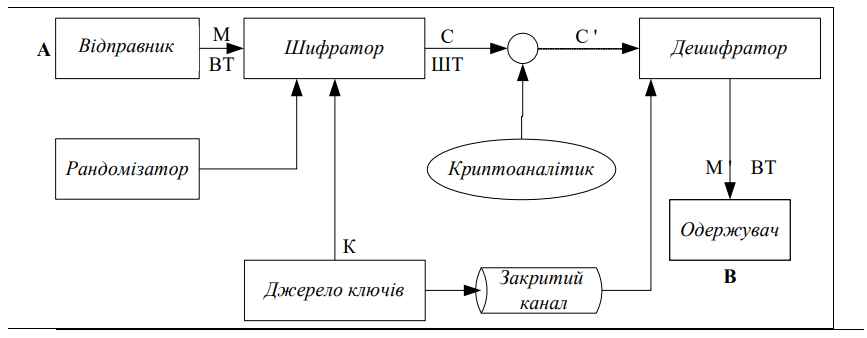
\includegraphics[width=0.8\linewidth]{Images/Secret_comunication_general_scheme.png}
    \caption{Caption}
    \label{fig:enter-label}
\end{figure}

















